% !TEX TS-program = xelatex
% !TEX encoding = UTF-8

% This is a simple template for a XeLaTeX document using the "article" class,
% with the fontspec package to easily select fonts.

\documentclass[oneside,10pt]{book} % use larger type; default would be 10pt

% other LaTeX packages.....

\usepackage{geometry} % See geometry.pdf to learn the layout options. There are lots.
\geometry{letterpaper} % or letterpaper (US) or a5paper or....
%\usepackage[parfill]{parskip} % Activate to begin paragraphs with an empty line rather than an indent

%\geometry{asymmetric}
\geometry{outer=2.5in}
\geometry{marginparwidth=2in}
\geometry{marginparsep=20pt}

% pour mettre des tableaux au bon endroit avec l'option H
%\usepackage{float}
% grands tableaux... pratiques
\usepackage{longtable}
 % pour faire des beaux tableaux
\usepackage{booktabs}
 
 % format des fonts comme Tufte
 \usepackage{xunicode} % Unicode support for LaTeX character names (accents, European chars, etc)
\usepackage{xltxtra} % Extra customizations for XeLaTeX
\usepackage{amsmath}
\usepackage{amsthm}
 \usepackage{fontspec}
\setmainfont[Renderer=Basic, Numbers=OldStyle, Scale = 1.0]{TeX Gyre Pagella}
\setsansfont[Renderer=Basic, Scale=0.90]{TeX Gyre Heros}
\setmonofont[Renderer=Basic]{TeX Gyre Cursor}


%\usepackage{marginnote}
%\renewcommand*{\raggedleftmarginnote}{}
%\renewcommand*{\raggedrightmarginnote}{}

% Margin Caption (done with sidenotes package)
% UTILISER \sidecaption pour une caption
%\usepackage[margincaption,rightcaption,ragged,wide]{sidecap}
%\usepackage[margincaption,outercaption]{sidecap}
%\sidecaptionvpos{figure}{t} 
%\sidecaptionvpos{table}{t}
% format des captions des figures
%\captionsetup[SCfigure]{format=plain, ...}
%\captionsetup[SCtable]{format=plain, ...}

\usepackage{sidenotes}

% bibliography
%\usepackage{natbib}
%\usepackage[notes,backend=biber]{biblatex-chicago}

%\usepackage[style=reading]{biblatex}
\usepackage[citestyle=reading,bibstyle=authortitle]{biblatex}

\addbibresource{Theo.bib}

%\bibliography{sample}
%\bibliography{siam}

%\newcommand*{\sidecite}[1]{\sidenote{[\cite{#1}].\citeauthor{#1} - \citetitle{#1}}


\usepackage{url}
\setlength\parindent{0pt}
% marginnote mn
\newcommand\mn[1]{\marginpar{\footnotesize #1}}

\newcommand\sn[1]{\sidenote{\footnotesize #1}}

%\usepackage{biblatex} %pour citer des numero de page
\usepackage[english,main=french]{babel}
\babelprovide[import]{arabic}
\babelfont[arabic]{rm}{Amiri}
\usepackage{arabtex}

%%% ToC (table of contents) APPEARANCE
\usepackage[nottoc,notlof,notlot]{tocbibind} % Put the bibliography in the ToC
\usepackage[titles,subfigure]{tocloft} % Alter the style of the Table of Contents
\renewcommand{\cftsecfont}{\rmfamily\mdseries\upshape}
\renewcommand{\cftsecpagefont}{\rmfamily\mdseries\upshape} % No bold!
%\newcommand\TArabe[1]{\foreignlanguage{arabic}{\RL}}
\newcommand\TArabe[1]{\foreignlanguage{arabic}{#1}}
\newcommand{\vide}[1]{}
%Recherche \hypertarget et remplacer par \vide
% \protect\hyperlink par \vide
%\texorpdfstring par RIEN
% \RL : \TArabe
% rechercher \footnote{ et remplacer par \sn{
% rechercher Al Gazali
% package pour faire des réferences à des labels pour le chapitre théologiens
\usepackage{cleveref}

% gros tableau
\usepackage{longtable}

\usepackage{eurosym}  %Euro
\usepackage[super]{nth} %for \nth{1} to give 1st
\usepackage{array} % permet de centrer les tableaux\

% Prints the month name (e.g., January) and the year (e.g., 2008)
\newcommand{\monthyear}{%
  \ifcase\month\or January\or February\or March\or April\or May\or June\or
  July\or August\or September\or October\or November\or
  December\fi\space\number\year
}


% Prints an epigraph and speaker in sans serif, all-caps type.
\newcommand{\openepigraph}[2]{%
  %\sffamily\fontsize{14}{16}\selectfont
  \begin{fullwidth}
  \sffamily\large
  \begin{doublespace}
  \noindent\allcaps{#1}\\% epigraph
  \noindent\allcaps{#2}% author
  \end{doublespace}
  \end{fullwidth}
}

% Inserts a blank page
\newcommand{\blankpage}{\newpage\hbox{}\thispagestyle{empty}\newpage}


%\splittopskip=5cm 

 





\usepackage[framemethod=TikZ]{mdframed}

\usepackage{thmtools}
\usepackage{blindtext} % avoid to cut theorem
% avoid to have theorem or definition in the list of theorm
\makeatletter
\patchcmd\thmt@mklistcmd
  {\thmt@thmname}
  {\check@optarg{\thmt@thmname}}
  {}{}
\patchcmd\thmt@mklistcmd
  {\thmt@thmname\ifx}
  {\check@optarg{\thmt@thmname}\ifx}
  {}{}
\protected\def\check@optarg#1{%
  \@ifnextchar\thmtformatoptarg\@secondoftwo{#1}%
}
\makeatother
% format of theorem
\declaretheoremstyle[
    headfont=\scshape, 
    notebraces={\scshape : }{.},
    bodyfont=\normalfont,
    headpunct={},
    postheadspace=\newline,
%    postheadhook={\textcolor{red}{\rule[.6ex]{\linewidth}{0.4pt}}\\},
    spacebelow=\parsep,
    spaceabove=\parsep,
    preheadhook={\begin{mdframed}[backgroundcolor=white!20, 
        splittopskip = \topskip,
            linecolor=blue!30, 
            linewidth = 2pt,
            innertopmargin=6pt,
            roundcorner=1pt, 
            innerbottommargin=6pt, 
            skipabove=\parsep,     
            skipbelow=\parsep]},
            postfoothook=\end{mdframed}]{Definitionstyle}


% example environment - thmtools


\declaretheorem[ style = Definitionstyle, name = {Definition}]{definition}
\declaretheorem[ style = Definitionstyle, name = {Definition}, sibling=definition]{Def}


\declaretheoremstyle[
    headfont=\scshape, 
    notebraces={\scshape : }{.},
    bodyfont=\normalfont,
    headpunct={},
    postheadspace=\newline,
%    postheadhook={\textcolor{red}{\rule[.6ex]{\linewidth}{0.4pt}}\\},
    spacebelow=\parsep,
    spaceabove=\parsep
]{Exercisestyle}
% example environment - thmtools



\declaretheorem[ style = Exercisestyle, name = Exemple ]{Ex}





%--------------------------------------------------------------
% Frame
%--------------------------------------------------------------

\usepackage[framemethod=TikZ]{mdframed}

\usepackage{thmtools}
%\usepackage{amsthm}

\usepackage{blindtext} % avoid to cut theorem
% avoid to have theorem or definition in the list of theorm
\makeatletter
\newcommand{\theosep}{\parsep}
\renewcommand{\theosep}{20pt}


%--------------------------------------------------------------
% Titre des listes de théorèmes
%--------------------------------------------------------------

\renewcommand{\listtheoremname}{List of Important Theorems}

\makeatletter
\def\ll@theorem{%
  \protect\numberline{\csname the\thmt@envname\endcsname}%
  \ifx\@empty\thmt@shortoptarg
    \thmt@thmname
  \else
    \thmt@shortoptarg
  \fi}
\def\l@thmt@theorem{} 
 \makeatother
 

% avoid to have theorem or definition in the list of theorm
\makeatletter
\patchcmd\thmt@mklistcmd
  {\thmt@thmname}
  {\check@optarg{\thmt@thmname}}
  {}{}
\patchcmd\thmt@mklistcmd
  {\thmt@thmname\ifx}
  {\check@optarg{\thmt@thmname}\ifx}
  {}{}
\protected\def\check@optarg#1{%
  \@ifnextchar\thmtformatoptarg\@secondoftwo{#1}%
}

 
\makeatother

% format of theorem


            
\declaretheoremstyle[
    headfont=\scshape, 
    notebraces={\scshape : }{.},
    bodyfont=\normalfont,
    headpunct={},
    postheadspace=\newline,
%    postheadhook={\textcolor{red}{\rule[.6ex]{\linewidth}{0.4pt}}\\},
    spacebelow=\parsep,
    spaceabove=\parsep,
    mdframed={
            backgroundcolor=white!20, 
            splittopskip = \topskip,
            linecolor=blue!30, 
            linewidth = 2pt,
            innertopmargin=\myinnertopmargin,
            roundcorner=1pt, 
            innerbottommargin=6pt, 
            skipabove=\parsep,     
            skipbelow=\parsep} 
    ]{Definitionstyle}
    
\declaretheoremstyle[
    headfont=\scshape, 
    notebraces={\scshape : }{.},
    bodyfont=\normalfont,
    headpunct={},
    postheadspace=\newline,
%    postheadhook={\textcolor{red}{\rule[.6ex]{\linewidth}{0.4pt}}\\},
    spacebelow=\parsep,
    spaceabove=\parsep,
    mdframed={backgroundcolor=white!20, 
            splittopskip = \topskip,
            linecolor=red!30, 
            linewidth = 2pt,
            innertopmargin=\myinnertopmargin,
            roundcorner=1pt, 
            innerbottommargin=6pt, 
            skipabove=\parsep,     
            skipbelow=\parsep} 
    ]{Propertystyle}

%,    postfoothook=
% example environment - thmtools
\declaretheoremstyle[
    headfont=\scshape, 
    notebraces={\scshape : }{.},
    bodyfont=\normalfont,
    headpunct={},
    postheadspace=\newline, 
%    postheadhook={\textcolor{red}{\rule[.6ex]{\linewidth}{0.4pt}}\\},
    spacebelow=\parsep,
    spaceabove=\parsep
]{Exercisestyle}
% example environment - thmtools

\declaretheoremstyle[
    headfont=\scshape, 
    notebraces={\scshape : }{.},
    bodyfont=\normalfont,
    headpunct={},
    postheadspace=\newline,
%    postheadhook={\textcolor{red}{\rule[.6ex]{\linewidth}{0.4pt}}\\},
    spacebelow=\parsep,
    spaceabove=\parsep,
    mdframed={backgroundcolor=gray!30, 
            splittopskip = \topskip,
            linecolor=red!30, 
            linewidth = 2pt,
            innertopmargin=\myinnertopmargin,
            roundcorner=1pt, 
            innerbottommargin=6pt, 
            skipabove=\parsep,     
            skipbelow=\parsep} 
    ]{TobeRetainedstyle}




\declaretheorem[ style = TobeRetainedstyle, name = {Synthèse} ]{Synthesis}


\declaretheorem[ style = Exercisestyle, numbered=no,name = Property]{property}
\declaretheorem[ style = Propertystyle, name = {Property} ]{Prop}
\declaretheorem[ style = Propertystyle, name = Theorem, sibling=Prop]{Theo}
\declaretheorem[ style = Propertystyle, name = Theorem, sibling=Prop]{theorem}
\declaretheorem[ style = Propertystyle, name = Lemma, sibling=Prop]{lemma}
\declaretheorem[ style = Exercisestyle, numbered=no,name = {Remark}]{rem}
\declaretheorem[ style = Definitionstyle, name = {Definition}]{definition}
\declaretheorem[ style = Definitionstyle, name = {Definition}, sibling=definition]{Def}
\declaretheorem[ style = Exercisestyle, name = Exercise]{exercise}
\declaretheorem[ style = Exercisestyle, name = Exercise, sibling=exercise]{Exercise}
\declaretheorem[ style = Exercisestyle, name = Exercise, sibling=exercise]{Exc}
\declaretheorem[ style = Exercisestyle, name = Exercise, sibling=exercise]{Exo}
\declaretheorem[ style = Exercisestyle, name = Problem, sibling=exercise]{problem}
\declaretheorem[ style = Exercisestyle, name = Example]{example}
\declaretheorem[ style = Exercisestyle, name = Example, sibling=example]{Ex}
\makeatother


%--------------------------------------------------------------
% Code
%--------------------------------------------------------------

%% Permet de mettre du code
\usepackage{listings}
\lstdefinestyle{mystyle}{
    basicstyle=\ttfamily\footnotesize,
    breakatwhitespace=false,         
    breaklines=true,                 
    captionpos=b,                    
    keepspaces=true,                 
    numbers=left,                    
    numbersep=5pt,                  
    showspaces=false,                
    showstringspaces=false,
    showtabs=false,                  
    tabsize=2
}
\lstset{%
	aboveskip=\topsep,
	belowskip=\topsep,
	xleftmargin=\parindent}

\lstset{style=mystyle}





\newcommand{\bi}{\begin{itemize}}
 \newcommand{\ei}{\end{itemize}}
  \newcommand{\be}{\begin{Ex}}
 \newcommand{\ee}{\end{Ex}}
 \newcommand{\mn}[1]{\marginnote{\footnotesize #1}}
  \newcommand{\sn}[1]{\sidenote{\footnotesize #1}}

\newcommand{\mzt}{\emph{muʿtazilite}}  
\newcommand{\CD}{\emph{la Cité de Dieu }}  

\newcommand{\CB}{\emph{Cedric Baylocq }} % nom du professeur
\newcommand{\riba}{\emph{Ribâ }}
\newcommand{\gharar}{\emph{Gharar }}


%Recherche \hypertarget et remplacer par \vide
% \protect\hyperlink par \vide
%\texorpdfstring par RIEN
% \RL : \TArabe
% rechercher \footnote{ et remplacer par \sn{
% rechercher Al Gazali
%\newcommand\TArabe[1]{\foreignlanguage{arabic}{\RL}}
\newcommand\TArabe[1]{\foreignlanguage{arabic}{#1}}
\newcommand\TGrec[1]{\foreignlanguage{greek}{#1}}
\newcommand{\vide}[1]{}

\renewcommand{\listtheoremname}{Liste des Definitions}

% Prints the month name (e.g., January) and the year (e.g., 2008)
\newcommand{\monthyear}{%
  \ifcase\month\or January\or February\or March\or April\or May\or June\or
  July\or August\or September\or October\or November\or
  December\fi\space\number\year
}

\newcommand{\tnote}{\textsuperscript}


% Inserts a blank page
\newcommand{\blankpage}{\newpage\hbox{}\thispagestyle{empty}\newpage}


% Prints an epigraph and speaker in sans serif, all-caps type.
\newcommand{\openepigraph}[2]{%
  %\sffamily\fontsize{14}{16}\selectfont
  \begin{fullwidth}
  \sffamily\large
  \begin{doublespace}
  \noindent\allcaps{#1}\\% epigraph
  \noindent\allcaps{#2}% author
  \end{doublespace}
  \end{fullwidth}
}
 


 

% Prints argument within hanging parentheses (i.e., parentheses that take
% up no horizontal space).  Useful in tabular environments.
\newcommand{\hangp}[1]{\makebox[0pt][r]{(}#1\makebox[0pt][l]{)}}
\newcommand{\hangstar}{\makebox[0pt][l]{*}}
%%
% Prints an asterisk that takes up no horizontal space.
% Useful in tabular environments.



% Macros for typesetting the documentation
\newcommand{\hlred}[1]{\textcolor{Maroon}{#1}}% prints in red
\newcommand{\hangleft}[1]{\makebox[0pt][r]{#1}}
\newcommand{\hairsp}{\hspace{1pt}}% hair space
\newcommand{\hquad}{\hskip0.5em\relax}% half quad space

\newcommand{\ie}{\textit{i.\hairsp{}e.}\xspace}
\newcommand{\eg}{\textit{e.\hairsp{}g.}\xspace}
\newcommand{\na}{\quad--}% used in tables for N/A cells

% Prints an epigraph and speaker in sans serif, all-caps type.





%%
\usepackage{graphicx} % support the \includegraphics command and options

\title{ISTR}
\author{Notes du Cours}
%\date{} % Activate to display a given date or no date (if empty),
         % otherwise the current date is printed 

\begin{document}

%\citestyle{verbose}


\maketitle

%-------------------------------------


\pagenumbering{roman} 
\setcounter{page}{1}
\begin{fullwidth}
\tableofcontents
\end{fullwidth}

\pagenumbering{arabic} 
\setcounter{page}{1}
 
\mainmatter



\part{Courants de l'Islam Contemporains - }
\chapter{Introduction}


\mn{Anne-Sophie Vivier Muresan \url{as.viviermuresan@icp.fr}
Anthropologue, THèse sur l'Iran, l'Islam en France
}
Ce cours porte sur les courants de l'Islam, depuis le XVII\textsuperscript{ème} siècle.

\paragraph{Processus}
Lire les textes


\paragraph{Validation} uniquement sur un thème lié au cours. utiliser Recherche+
Un écrit en format Word.



\section{Chronologie indicative}

 
\paragraph{1744 } Alliance entre Muhammad Ibn ‘Abd el-Wahhab, fondateur de la doctrine wahabbite, et Ibn Sa‘ud, ancêtre de la dynastie saoudienne actuelle.

\paragraph{1798} : Expédition en Egypte de Napoléon. Date-symbole habituellement retenue pour marquer le début de l’intensification des relations réciproques entre Occident et Orient musulman.
\paragraph{1826-1831 }: l’Etat égyptien envoie un groupe de 40 personnes étudier en France. La modernité est alors comprise comme appropriation des sciences développées en Occident.
\paragraph{1830 } : Prise d’Alger par la France. Début de la main mise de l’Occident sur le monde arabe (colonisation et mandats).
\paragraph{1839 } : Début des « réformes » modernisatrices (tanzimat) dans l’Empire Ottoman. La modernité est pensée en termes de réformes sociales et politiques sur le modèle occidental.
\paragraph{1884 } : Jamal ad-din al-Afghani et Mohammad Abduh fondent à Paris la revue Al ‘Urwa al Wuthqa. Débuts du mouvement réformiste musulman.
\paragraph{1924 } : prise de La Mecque et de Médine par les descendants d’Ibn Sa’ud et de Muhammad Ibn Abd al Wahhab. L’Arabie Saoudite devient le foyer du fondamentalisme musulman, qu’elle propagera surtout à partir des années 1970.
\paragraph{1924 } : abolition du califat par Mustapha Kemal (Atatürk). Recherche d’un accord au sein du monde sunnite pour l’élection d’un nouveau calife, sans suite.
\paragraph{1929 } : Fondation des Frères Musulmans par Hassan al-Banna, en Egypte. Vise l’ « islamisation par le bas », par l’éducation religieuse et la da‘wa (activité missionnaire).
\paragraph{1941 } : Fondation de l’association Jama‘at al-islami par Mawdudi au Pakistan. Débuts de l’islam politique (islamisme).
\paragraph{1947 } : Création du Pakistan, premier Etat moderne fondé sur une définition d’abord musulmane de la Nation.
\paragraph{1979-80 } : Révolution iranienne et instauration de la République islamique. En parallèle, montée en puissance des islamistes dans de nombreux pays musulmans.
\paragraph{1985 } : Pendaison de Mahmud Taha, au Soudan, accusé de blasphème pour son interprétation novatrice de la Révélation coranique. Emergence des « nouveaux penseurs de l’islam », qui cherchent à rompre avec la visée réformiste et à repenser entièrement le rapport de l’islam à la modernité.
\paragraph{2001 } : Attentat du 11 septembre. L’islam politique, qui a perdu sa légitimité au sein du monde musulman, se radicalise, se sectarise, et prend la voie du terrorisme.

\paragraph{2007 } : « Lettre des 138 » : 138 théologiens musulmans affirment leur désir de dialogue et de paix dans une lettre adressée aux responsables religieux chrétiens. C’est la première fois qu’une voix commune de cette ampleur prend corps en islam.
\paragraph{2014 } : Victoires de Da’esh (Etat Islamique) en Irak et en Syrie. Prétentions à l’instauration d’un califat – refusé par l’ensemble des savants et des institutions sunnites officielles.
 
%\hypertarget{second-semestre-2021-2022}{%
\section{Second semestre 2021-2022}\label{second-semestre-2021-2022}}

\begin{quote}
Anne-Sophie Vivier-Mureşan

Documents annexes au cours
\end{quote}

\hypertarget{indications-pedagogiques}{%
\subsection{INDICATIONS PEDAGOGIQUES}\label{indications-pedagogiques}}

\begin{enumerate}
\def\labelenumi{\arabic{enumi}.}
\item
  \begin{quote}
  \textbf{Préparation des cours}
  \end{quote}
\end{enumerate}

\begin{quote}
Chaque cours s'appuiera sur la lecture d'un (ou deux) texte(s)
significatif(s) pour le thème abordé. Il est demandé aux étudiants
d'avoir lu le texte à l'avance de façon suffisamment approfondie pour
pouvoir réagir aux questions abordées en cours.
\end{quote}

\hypertarget{approfondissement-des-cours}{%
\subsection{Approfondissement des
cours}\label{approfondissement-des-cours}}

\begin{quote}
En complément de chaque cours, un ou plusieurs documents seront mis en
ligne pour approfondissement (plate-forme e-learning à partir du site :
{https://formation.icp.fr/})
\end{quote}

\hypertarget{validation}{%
\subsection{Validation}\label{validation}}

\begin{quote}
La validation pourra prendre la forme suivante, au choix :
\end{quote}

\begin{enumerate}
\def\labelenumi{\alph{enumi}.}
\item
  \begin{quote}
  {Un dossier sur un thème lié au cours}
  \end{quote}
\end{enumerate}

\begin{quote}
A partir de trois articles universitaires minimum.
\end{quote}

\begin{itemize}
\item
  \begin{quote}
  Introduction : intérêt du thème au regard de l'actualité et/ou de vos
  propres orientations personnelles ; présentation des articles et de
  leurs auteurs. Présentation du plan de votre travail.
  \end{quote}
\item
  \begin{quote}
  Synthèse (ne pas présenter les articles séparément mais faire une
  synthèse à partir des différentes thématiques rencontrées)
  \end{quote}
\item
  \begin{quote}
  Contextualisation de ce thème dans l'islam contemporain, éclairage par
  le contenu du cours (enjeux, dynamiques, etc).
  \end{quote}
\end{itemize}

\begin{enumerate}
\def\labelenumi{\alph{enumi}.}
\setcounter{enumi}{1}
\item
  \begin{quote}
  {Une question d'actualité} (sauf masters)
  \end{quote}
\end{enumerate}

\begin{quote}
A partir de trois articles journalistiques minimum.
\end{quote}

\begin{itemize}
\item
  \begin{quote}
  Introduction : brève historique et/ou recontextualisation de la
  question ; présentation des médias utilisés. Présentation du plan de
  votre travail.
  \end{quote}
\item
  \begin{quote}
  Synthèse (ne pas présenter les articles séparément mais faire une
  synthèse à partir des différentes thématiques rencontrées).
  \end{quote}
\item
  \begin{quote}
  Eclairage à partir des données du cours (compléments d'information,
  regard critique, etc.)
  \end{quote}
\end{itemize}

\hypertarget{modalituxe9s}{%
\subsection{Modalités :}\label{modalituxe9s}}

\begin{quote}
La validation peut se faire par oral ou par écrit (sauf pour les
étudiants de master, pour qui un écrit est requis) :
\end{quote}

\begin{itemize}
\item
  \begin{quote}
  Un oral : présentation du travail en 20 mn, suivies de 10 mn de
  questions
  \end{quote}
\item
  \begin{quote}
  Un écrit : de 5 pages maximum, \textbf{remis le 27 mai 2022} au plus
  tard en format numérique sur Moodle (boîte de dépôt) \textbf{: format
  Word}, pour me permettre d'intégrer ma note et mes remarques.
  \end{quote}
\end{itemize}

\begin{quote}
\textbf{NB} : \textbf{La présentation orale comme écrite devra être
structurée} : introduction, plan rigoureux, conclusion. \textbf{La
présentation orale doit inclure la présentation écrite} du plan de
l'exposé (avec intitulé du sujet ou de l'œuvre choisie et nom de
l'étudiant).



pratiquement, choisir un sujet qui nous intéresse. le proposer à la pause.
Ce qui sera important, c'est de montrer qu'on a assimilé le cours.


\section{Programme des Cours}
\end{quote}


\hypertarget{la-violence-luxe9gitimuxe9e-de-la-ruxe9volution-aux-attentats-suicide-14032022}{%
\subsection{\texorpdfstring{{La violence légitimée : de la
révolution aux attentats-suicide}
\emph{(14/03/2022)}}{La violence légitimée : de la révolution aux attentats-suicide (14/03/2022)}}\label{la-violence-luxe9gitimuxe9e-de-la-ruxe9volution-aux-attentats-suicide-14032022}}

\begin{quote}
BENICHOU David, KHOSROKHAVAR Farhad, MIGAUX Philippe \emph{Le jihadisme.
Le comprendre pour mieux le combattre}, Plon, Paris, 2015.

BENSLAMA Fethi et KHOSROKHAVAR Farhad, \emph{Le djihadisme des femmes},
Paris, Seuil, 2017. BONNER, Michael \emph{Le jihad. Origines,
interprétations, combats}, Téraèdre, 2004.

CARRE, Olivier \emph{Mystique et politique : le Coran des islamistes,
commentaire coranique de Sayyid Qutb}, Cerf, Paris, 2004.

KEPEL, Gilles \emph{La revanche de Dieu: chrétiens, juifs et musulmans à
la reconquête du monde}, Seuil, Paris, 1991. Sur l'islam, p. 32-81.

*\emph{Du jihad à la fitna}, Bayard, Paris, 2005.

KEPEL, Gilles ; MILELLI, Jean-Pierre \emph{Al-Qaida dans le texte}, PUF,
Paris, 2008.

LUIZARD Pierre-Jean, \emph{Le piège Da'ech, l'Etat islamique ou le
retour de l'Histoire}, La Découverte, Paris, 2015.
\end{quote}

\begin{enumerate}
\def\labelenumi{\arabic{enumi}.}
\setcounter{enumi}{1}
\item
  \begin{quote}
  \textbf{{Le chiisme : histoire et doctrines}}
  \emph{(21/03/2022)}
  \end{quote}
\end{enumerate}

\begin{quote}
AMIR-MOEZZI, M-A. \emph{La religion discrète : croyances et pratiques
spirituelles dans l'Islam shi'ite}, Vrin, Paris, 2006.

AMIR-MOEZZI, M-A. et JAMBET, Christian \emph{Qu'est-ce que le shî'isme
?}, Fayard, Paris, 2004.

CORBIN, Henry \emph{En islam iranien: aspects spirituels et
philosophiques,} 4 volumes, Gallimard, Paris, 1991.

HALM, Heinz \emph{Le Chiisme}, Paris, PUF, 1995.

RICHARD, Yann \emph{L'islam chi'ite : croyances et idéologies}, Fayard,
Paris, 1991.

*TABATABA'I, Muhammad Huseyn \emph{Le chiisme en islam}, Beyrouth,
Al-Bouraq, 2009.
\end{quote}

\hypertarget{le-chiisme-au-xxe-siuxe8cle-de-la-ruxe9forme-uxe0-la-ruxe9volution-28032022}{%
\subsection{\texorpdfstring{{Le chiisme au XXe siècle : de la
réforme à la révolution}
\emph{(28/03/2022)}}{Le chiisme au XXe siècle : de la réforme à la révolution (28/03/2022)}}\label{le-chiisme-au-xxe-siuxe8cle-de-la-ruxe9forme-uxe0-la-ruxe9volution-28032022}}

\begin{itemize}
\item
  \begin{quote}
  KHOMEYNI, Ruhollah \emph{Gouvernement islamique}, Institut pour
  l'édition et la publication des œuvres de l'ayatollah Khomeyni,
  Téhéran, 1996.
  \end{quote}
\item
  \begin{quote}
  SHARIATI, Ali \emph{Histoire et destinée} {[}textes choisis{]},
  Sindbad, Paris, 1982.
  \end{quote}
\end{itemize}

\begin{quote}
\emph{Fatima est Fatima}, Albouraq, Beyrouth, 2009.

ADELKHAH, Fariba \emph{La révolution sous le voile}, Karthala, Paris,
1991.

*ADELKHAH, Fariba ; BAYART, Jean-François ; ROY, Olivier \emph{Thermidor
en Iran}, Ed. Complexes, Bruxelles, 1993.

*DIGARD, Jean-Pierre ; HOURCADE, Bernard ; RICHARD, Yann \emph{L'Iran au
XXe siècle}, Fayard, Paris, 2007.

KIAN-THIEBAUT, Azadeh \emph{La République islamique d'Iran : de la
maison du Guide à la raison d'Etat}, Michalon, Paris, 2005.

KHOSROKHAVAR, Farhad \emph{L'utopie sacrifiée, sociologie de la
Révolution iranienne}, Presses de la Fondation Nationale des Sciences
Politiques, Paris, 1993.

*KHOSROKHAVAR, Farhad et ROY, Olivier : \emph{Iran, comment sortir d'une
révolution religieuse ?}, Seuil, Paris, 1999.

MERVIN, Sabrina \emph{Un réformisme chiite. Ulémas et lettrés du Gabal
`Amil (actuel Liban-Sud) de la fin de l'Empire ottoman à l'indépendance
du Liban}, Karthala-CERMOC - IFEAD, Paris-Beyrouth-Damas, 2000.

MERVIN, Sabrina (dir.) \emph{Les mondes chiites et l'Iran}, Paris,
Karthala-IFPO, 2007.
\end{quote}

\begin{enumerate}
\def\labelenumi{\arabic{enumi}.}
\item
  \begin{quote}
  \textbf{{La nouvelle pensée islamique}} \emph{(04/04/2022)}
  \end{quote}
\end{enumerate}

\begin{itemize}
\item
  \begin{quote}
  AL AJAMI, \emph{Que dit vraiment le Coran}, Erick Bonnier Editions,
  2020.
  \end{quote}
\item
  \begin{quote}
  ABOU ZEID Nasr Hamid \emph{Critique du discours Religieux}, Sindbad,
  Acte Sud, Paris, 1999.
  \end{quote}
\item
  \begin{quote}
  AL-BANNA, Gamal \emph{L'Islam, la Liberté, la Laïcité et le Crime de
  la tribu des « il nous a été rapporté »}, trad. D. Avon et A. Elias,
  L'Harmattan, Paris, 2013.
  \end{quote}
\item
  \begin{quote}
  ARKOUN, Mohamed \emph{Lectures du Coran}, Maisonneuve \& Larose,
  Paris, 1982.
  \end{quote}
\item
  \begin{quote}
  BAJRAFIL, Mohammed \emph{L'islam de France, l'an I. Il est temps
  d'entrer dans le XXIe siècle}, Ed. Plein Jour, 2015.
  \end{quote}
\item
  \begin{quote}
  BENKIRANE Réda \emph{Islam, à la reconquête du sens}, éd. Le Pommier,
  2017.
  \end{quote}
\item
  \begin{quote}
  CHARFI, Abdelmajid \emph{L'islam entre le message et l'histoire},
  Albin Michel, Paris, 2004.
  \end{quote}
\end{itemize}

\begin{quote}
\emph{La pensée islamique, ruptures et fidélités}, Albin Michel, 2008.
\end{quote}

\begin{itemize}
\item
  \begin{quote}
  CHEBEL, Malek \emph{Manifeste pour un islam des lumières}, Hachette,
  Paris, 2004.
  \end{quote}
\item
  \begin{quote}
  ESACK Farid \emph{Coran, mode d'emploi}, Albin Michel, Paris, 2004.
  \end{quote}
\item
  \begin{quote}
  LAMRABET Asma, \emph{Islam et femmes : les questions qui fâchent},
  Casablanca, En toutes lettres, 2017.
  \end{quote}
\item
  \begin{quote}
  SANGARE, Youssouf \emph{Repenser le Coran et la tradition islamique --
  Introduction à la pensée de Fazlur Rahman}, Al Bouraq, 2017.
  \end{quote}
\item
  \begin{quote}
  TALBI Mohamed \emph{Plaidoyer pour un Islam moderne}, Cérès/Tunis,
  DDB/Paris, 1998.
  \end{quote}
\end{itemize}

\begin{quote}
*BENZINE, Rachid \emph{Les nouveaux penseurs de l'Islam}, Albin Michel,
Paris, 2004. FILALI-ANSARY, Abdou \emph{Réformer l'islam ? Une
introduction aux débats contemporains}, La

Découverte, Poche, Paris, 2005.

*HOFFNER, Anne-Bénédicte \emph{Les nouveaux acteurs de l'islam}, Paris,
Bayard, 2017.

RENAUD, Etienne "Mahmud Taha et la «seconde mission de l'Islam»",
\emph{Se Comprendre}, 85/07, 1985.

ROUSSILLON\textbf{,} Alain \emph{La pensée islamique contemporaine},
\emph{acteurs et enjeux}, Téraèdre, Paris, 2005.

SALEH Waël, \emph{A la recherche d'un aggiornamento de l'islam. Des
voies contemporaines}, Paris, L'Harmattan, 2018.
\end{quote}

\begin{enumerate}
\def\labelenumi{\arabic{enumi}.}
\setcounter{enumi}{1}
\item
  \begin{quote}
  \textbf{{La réforme du droit}} \emph{(11/04/2022)}
  \end{quote}
\end{enumerate}

\begin{quote}
ARMINJON, Constance \emph{Les droits de l'Homme dans l'islam shi'ite.
Confluences et lignes de partage}, Paris, Éditions du Cerf, 2017.

BABES, L. ; OUBROU, T. \emph{Loi d'Allah, loi des hommes}, Albin Michel,
Paris, 2002.

BEN ACHOUR, Yadh \emph{Normes, foi et loi - en particulier dans
l'Islam}, Ceres, Tunis, 1993.

\emph{La deuxième Fâtiha. L'islam et la pensée des droits de l'homme},
PUF, Paris, 2011.

BENKHEIRA, M.H. \emph{L'amour de la Loi - Essai sur la normativité en
islam}, Puf, Paris, 1997.

*CARRE, Olivier \emph{L'Islam laïque ou le retour à la Grande
Tradition}, Armand Colin, Paris, 1993.

*DUPRET Beaudoin \emph{La charia. Des sources à la pratique, un concept
pluriel}, Paris, La Découverte, 2014.

DUPRET, Beaudoin (dir.) \emph{La charia aujourd'hui. Usage de la
référence au droit islamique}, Paris, La Découverte, 2012.

YOUNES Michel (dir.) \emph{La fatwa en Europe. Droit de minorité et
enjeux d'intégration}, Profac, Lyon, 2010.
\end{quote}

\begin{enumerate}
\def\labelenumi{\arabic{enumi}.}
\setcounter{enumi}{2}
\item
  \begin{quote}
  \textbf{{Le soufisme au XXe siècle}} \emph{(09/05/2022)}
  \end{quote}
\end{enumerate}

\begin{quote}
\emph{*Réveils du soufisme en Afrique et en Asie}, dossier de la revue
\emph{Archives de Sciences Sociales des Religions}, n° 135, 2006.

\emph{Confréries soufies en métropole}, dossier de la revue
\emph{Archives de Sciences Sociales des Religions}, n° 140, 2007.

AMSELLE, Jean-Louis \emph{Islams africains : la préférence soufie},
Jean-Louis Amselle, Paris, éd. du Bord de l'eau, 2017.

BALCI, Bayram \emph{Missionnaires de l'islam en Asie Centrale : les
écoles turques de Fethullah Gülen}, Paris, Maisonneuve et Larose, 2003.

CHIH, Rachida \emph{Le soufisme au quotidien : confréries d'Egypte au
XXe siècle}, Paris : Sindbad, Arles, Actes Sud, 2000.

FATHI, Habiba « Les réseaux mystiques au Kazakhstan : entre zhikr et
militantisme ? », \emph{Cahiers d'Asie Centrale}, n° 15-16, 2007, p.
223-261.

GEOFFROY, Eric « Soufisme, réformisme et pouvoir en Syrie contemporaine
», \emph{Egypte/Monde Arabe}, n° 29, 1997, p. 11-22.

*\emph{Le soufisme - Histoire, fondements et pratiques de l'islam
spirituel}, Paris, Eyrolles, 2019.

POPOVIC, A. ; VEINSTEIN, G. (dir.) \emph{Les voies d'Allah : les ordres
mystiques dans l'Islam des origines à aujourd'hui}, Paris, Fayard, 1996.

ROMEY, Alain « Rôle du wahabisme et du réformisme de la Nahda en Algérie
dans le processus d'exclusion et de marginalisation du soufisme »,
\emph{Cahiers de la Méditerranée}, 69, 2004,
\url{http://cdlm.revues.org/index735.html}

Les courants de l'islam contemporain (1)
\end{quote}

\hypertarget{introduction-guxe9nuxe9rale-du-cours}{%
\subsection{Introduction générale du
cours}\label{introduction-guxe9nuxe9rale-du-cours}}

\begin{enumerate}
\def\labelenumi{\Roman{enumi}.}
\item
  \begin{quote}
  \textbf{L'islam, une religion mondiale}
  \end{quote}

  \begin{enumerate}
  \def\labelenumii{\arabic{enumii}.}
  \item
    \begin{quote}
    L'expansion de l'islam
    \end{quote}
  \item
    \begin{quote}
    Répartition démographique
    \end{quote}
  \end{enumerate}
\item ~
  \hypertarget{une-grande-diversituxe9-confessionnelle}{%
  \subsection{Une grande diversité
  confessionnelle}\label{une-grande-diversituxe9-confessionnelle}}

  \begin{enumerate}
  \def\labelenumii{\arabic{enumii}.}
  \item
    \begin{quote}
    Sunnisme, chiisme et autres « confessions »
    \end{quote}
  \item
    \begin{quote}
    Au sein du sunnisme : les différentes écoles de droit
    \end{quote}
  \end{enumerate}
\item ~
  \hypertarget{diversituxe9-des-formes-culturelles.-quelques-exemples.}{%
  \subsection{Diversité des formes culturelles. Quelques
  exemples.}\label{diversituxe9-des-formes-culturelles.-quelques-exemples.}}

  \begin{enumerate}
  \def\labelenumii{\arabic{enumii}.}
  \item
    \begin{quote}
    La mosquée
    \end{quote}
  \item
    \begin{quote}
    Le vêtement féminin
    \end{quote}
  \item
    \begin{quote}
    Approche anthropologique : texte de Clifford Geertz.
    \end{quote}
  \end{enumerate}
\end{enumerate}

\hypertarget{glossaire}{%
\subsection{\texorpdfstring{{Glossaire}}{Glossaire}}\label{glossaire}}

\begin{quote}
{Personnes} Bukhari Ghazali

Ibn Sina (Avicenne) Mu`awiyya

Rumi

{Lieux} Siffîn

{Islam non sunnite} Alévis

Druzes Ghulât Ismaéliens

Kharijites/ibadites Zaydites

{Ecoles de droit sunnites} Hanbalites

Hanéfites Malékites Shafi`ites

{Autres termes} hijab

mihrab minbar qibla

 
\end{quote}
 

\begin{enumerate}
\def\labelenumi{\Roman{enumi}.}
\item ~
  \hypertarget{un-pensuxe9e-fondatrice-sayyid-qutb-1906-1966}{%
  \subsection{\texorpdfstring{{Un pensée fondatrice : Sayyid
  Qutb
  (1906-1966)}}{Un pensée fondatrice : Sayyid Qutb (1906-1966)}}\label{un-pensuxe9e-fondatrice-sayyid-qutb-1906-1966}}

  \begin{enumerate}
  \def\labelenumii{\arabic{enumii}.}
  \item
    \begin{quote}
    Une vie de militant
    \end{quote}
  \item
    \begin{quote}
    Le \emph{Fi zilâl al-Qur'an} : une méthode de lecture du Coran
    \end{quote}
  \item
    \begin{quote}
    L'Etat islamique : une utopie
    \end{quote}
  \end{enumerate}
\end{enumerate}

\begin{quote}
5. Place centrale du \emph{jihad}
\end{quote}

\begin{enumerate}
\def\labelenumi{\Roman{enumi}.}
\setcounter{enumi}{1}
\item ~
  \hypertarget{les-duxe9rives-djihadistes}{%
  \subsection{\texorpdfstring{{Les dérives
  djihadistes}}{Les dérives djihadistes}}\label{les-duxe9rives-djihadistes}}

  \begin{enumerate}
  \def\labelenumii{\arabic{enumii}.}
  \item
    \begin{quote}
    La première génération : la guérilla.
    \end{quote}
  \item
    \begin{quote}
    La deuxième génération : le terrorisme mondial.
    \end{quote}
  \item
    \begin{quote}
    Da`esh, troisième génération du djihadisme
    \end{quote}
  \item
    \begin{quote}
    Le martyre : quelle légitimité ?
    \end{quote}
  \end{enumerate}
\end{enumerate}

\hypertarget{glossaire-4}{%
\subsection{\texorpdfstring{{Glossaire}}{Glossaire}}\label{glossaire-4}}

\begin{quote}
{Personnes}

Al-Zawahiri (Ayman) Ben Laden (Usama) Farag (Abd as-salam) Ibn Taymiyya
Mawdudi

Nadawi

Qaradawi (Sheykh) Tantawi (Sheikh)

{Autres noms propres} Al-Jazira/ Al-Jazeera Dar-al-ulum

Hamas

Harakat al-jihad al-islami Hezbollah

kharijites

{Notions}

dar al-harb: \emph{territoire de la guerre}

dar al-islam: \emph{territoire de l'islam}

dar al-kufr: \emph{territoire des infidèles (mot-à- mot : territoire de
l'impiété)}

dar as-sulh: \emph{territoire de la paix}

dhimmi : « protégés » (statut particulier accordé aux chrétiens et aux
juifs) fasiq: \emph{pécheur}

fiqh: \emph{droit (musulman)}

fitna: \emph{discorde, querelle (conflit interne au monde musulman)}

hakimiyya : \emph{souveraineté}

hijra : \emph{exode}

`ibada : \emph{culte}

ijtihad : \emph{effort personnel d'interprétation (des textes sacrés)}

isnad : \emph{chaîne de transmission (des hadiths)} jahiliyya :
\emph{ignorance =\textgreater{} société païenne, impie}

kafir/kufr : \emph{impie/impiété}

munafiq : \emph{hypocrite (désigne l'ennemi}

\emph{« interne » à l'umma)}

na'ib : \emph{délégué} qatl : \emph{meurtre} shahid : \emph{martyr}

shura : \emph{principe de consultation}

taghut : \emph{tyran}

`ubudiyya : \emph{servitude}

umma : \emph{communauté musulmane}
\end{quote}

\hypertarget{sayyid-qutb-1906-1966}{%
\subsection{\texorpdfstring{{Sayyid Qutb
(1906-1966)}}{Sayyid Qutb (1906-1966)}}\label{sayyid-qutb-1906-1966}}

\begin{quote}
UNE GENERATION CORANIQUE UNIQUE

\textbf{Il y a un phénomène historique devant lequel doivent s'arrêter
les détenteurs de l'appel de l'islam en tout lieu et en tout temps.} Et
ils doivent s'y arrêter longuement. En effet, cela a une influence
décisive sur la méthode et l'orientation de l'appel. \textbf{Cet appel a
formé une génération de gens, la génération des compagnons (que la
satisfaction de Dieu soit sur eux), une génération distinguée dans toute
l'histoire de l'Islam et dans l'histoire de l'humanité toute entière.
Depuis il n'a jamais été formé ce type {[}d'homme{]} une autre fois}.
Oui, on trouve des individus de ce type dans le cours de l'histoire,
mais il n'est jamais arrivé que se rassemble un si grand nombre, en un
seul endroit, comme il y avait dans cette première période de la
génération de cet appel. Ceci est un phénomène clair et actuel, il
possède une signification devant laquelle il faut s'arrêter longuement ;
peut-être découvrirons-nous son secret. Le Coran de cet appel est entre
nos mains ; le hadith du Messager de Dieu, (la bénédiction de Dieu et la
paix soient sur Lui), son enseignement pratique, sa noble biographie,
sont aussi entre nos mains, comme ils étaient entre les mains de cette
première génération - laquelle ne s'est pas répétée dans l'histoire-...
Rien n'a disparu {[}aujourd'hui{]}, sauf la personne du Messager de
Dieu, (la bénédiction de Dieu et la paix soient sur Lui). Alors, est-ce
cela le secret ? Si l'existence du Messager de Dieu, (la bénédiction de
Dieu et la paix soient sur Lui) était inévitable pour la mise en place
de cet appel, et pour porter ses fruits ; Dieu n'en aurait pas fait un
appel à tous les hommes, et n'en aurait pas fait un dernier message,
n'en aurait pas fait dépendre les affaires des hommes sur terre jusqu'à
la fin des temps. Mais Dieu (qu'il soit honoré) s'est engagé par la
conservation de l'invocation et il a su que cet appel pouvait continuer
après le Messager de Dieu, (la bénédiction de Dieu et la paix soient sur
Lui) et pouvait porter ses fruits. Il l'a rappelé auprès de lui après 23
ans de mission et a fait rester sa religion depuis après lui jusqu'à la
fin des temps. L'absence de la personne du Messager de Dieu, (la
bénédiction de Dieu et la paix soient sur Lui) n'explique donc pas ce
phénomène et n'en donne pas la raison.

* * *

Cherchons donc une autre cause. \textbf{Regardons la source a laquelle a
puisé cette première génération, peut-être que quelque chose a changé en
elle}. Et regardons dans la voie qui les a formés ; peut-être que
quelque chose a changé en elle pareillement.

\textbf{Cette première source a laquelle a puisé cette génération, c'est
la source du Coran. Rien que le Coran}. Alors, le hadith du Messager de
Dieu, (la bénédiction de Dieu et la paix soient sur Lui), et son
enseignement, n'ont été qu'une des traces de cette source. Et quand on a
interrogé Aïsha (que Dieu soit satisfait d'elle) au sujet de l'éthique
du Messager de Dieu, (la bénédiction de Dieu et la paix soient sur Lui),
elle a dit: ``\textbf{Son éthique était le Coran}''\textbf{Le Coran seul
donc, était la source à laquelle ils ont puisé, par laquelle ils sont
devenus conditionnés, par laquelle ils ont été formés. Ceci n'a pas été
ainsi parce qu'à ce jour, l'humanité n'avait ni civilisation, ni
culture, ni science, ni écrits, ni études... Non ! Au contraire, il y
avait la civilisation romaine, sa culture, ses lois, desquelles l'Europe
continue à vivre (ou de ses extensions)}. Et il y avait les vestiges de
la civilisation grecque, sa logique, sa philosophie, son art et c'est ce
qui continue à irriguer la pensée occidentale jusqu'à aujourd'hui. Et il
y avait de même la civilisation perse, son art, sa poésie, sa
mythologie, ses dogmes et son système de gouvernement. Et d'autres
civilisation lointaines et proches : la civilisation hindoue, la
civilisation chinoise, etc. Et les deux civilisations romaines et perses
étaient au bord de la péninsule arabique, à son nord et à son sud, de
même que les juifs et les chrétiens vivaient au coeur de la péninsule...
\textbf{Ce n'est donc pas à cause de la pauvreté des civilisations
mondiales, des cultures mondiales que cette génération s'est limitée au
Livre de Dieu uniquement, dans la période de formation. il y avait là
une intention spécifique, une direction voulue.}

La colère du Messager de Dieu, (la bénédiction de Dieu et la paix soient
sur Lui) a montré cette intention quand il a vu dans la main de Omar ben
Khatâb (que Dieu soit satisfait de lui), une copie de la Torah. Alors,
il a dit : Si Moïse avait vécu parmi vous, il ne lui aurait pas été
permis autre chose que me suivre.''\textbf{Il y avait donc l'intention
de la part du Messager de Dieu, (la bénédiction de Dieu et la paix
soient sur Lui) de limiter la source à laquelle a puisé cette
génération, dans cette première période de formation, au Livre de Dieu
uniquement, pour que leurs âmes soient pour Lui seul, et pour que leur
comportement se redresse sur sa voie à Lui seul.} D'où le fait qu'il est
devenu furieux quand il a vu Omar ben Khatâb (que Dieu soit satisfait de
lui), puiser à d'autre source. Le Messager de Dieu, (la bénédiction de
Dieu et la paix soient sur Lui) a voulu faire une génération pure de
coeur, pure d'esprit, pure d'appréhension, pure de sentiment, pure de la
formation de toute influence autre que celle de la direction divine que
contient le Saint Coran. \textbf{Cette génération a puisé donc à cette
unique source ; ce pourquoi elle a eu dans l'histoire ce statut
unique... Alors, que s'est-il passé ? Les sources se sont mélangées. Se
sont déversé dans la source à laquelle a puisé les générations
suivantes, la philosophie des grecs et leur logique, la mythologie perse
et ses conceptions, les ``judaïtés'' juive et la théologie chrétienne et
d'autres éléments d'autres civilisations et cultures. Tout cela était
mélangé avec le \emph{tafsîr} du Coran, et la science du \emph{Kalâm},
comme c'était mélangé avec le \emph{fiqh} et la croyance. Toutes les
générations, après celle-ci ont été formées à cette source polluée, si
bien que cette génération ne s'est jamais répétée}. Et il ne fait pas de
doute que le mélange de cette source première a été un des facteurs
fondamentaux de cette différence entre toutes ces générations et la
génération distincte et unique.

* * *

\textbf{Il y a un autre fait fondamental, autre que la différence de
nature de la source. C'est la manière différente de recevoir ce qui a
formé cette génération unique et distincte}. Ceux de la première
génération \textbf{ne lisaient pas le Coran avec la volonté
{[}d'acquérir{]} une culture ou un savoir, ni avec la volonté du goût et
de la jouissance. Aucun d'entre eux n'a reçu le Coran pour augmenter sa
provision de culture, juste pour la culture, et ne remplissaient une
réserve de propositions scientifiques et juridiques. En effet, il
recevait le Coran pour recevoir un ordre de Dieu concernant ses affaires
et les affaires de la communauté dans laquelle il vivait. Il recevait
cet ordre pour le mettre en pratique dès qu'il l'entendait, comme un
soldat reçoit l'ordre du jour dans un champ de bataille pour le mettre
en pratique sitôt reçu.} En conséquence, il n'y avait aucun d'entre eux
pour {[}chercher{]} à augmenter ces {[}réserves{]} d'un seul coup, parce
qu'il sentait que cela augmentait les devoirs et les fardeaux qu'il
devait charger sur ses épaules et il se limitait à dix versets afin de
les garder et d'y travailler (comme il est dit dans le hadith de Ibn
Mas'ud (que Dieu soit satisfait de lui) \textbf{Cette attitude . . .
cette attitude de recevoir pour la mise en pratique. . . leur ouvrait
dans le Coran les horizons de la joie, horizons du savoir, qui
n'auraient pas été ouverts s'ils avaient misé sur lui avec une attitude
de recherche, d'études et de connaissance. Cela rendait facile le
travail et rendait léger les fardeaux. Le Coran était mélangé avec leur
identité, était transformé dans leurs âmes et leur vie, en un chemin
concret, en une culture dynamique qui ne reste pas à l'intérieur des
esprits ni sur le papier, mais se change en effets et en événements qui
modifie la trajectoire de la vie.} Le Coran ne livre ses trésors qu'à
ceux qui viennent à lui avec cet esprit : esprit de connaissance
engendrant une pratique. Il ne vient pas pour être un livre de plaisir
intellectuel, ni un livre de lettre et d'art, ni un livre d'histoires ou
d'histoire (même si tout ceci est contenu dedans), mais il vient pour
être un chemin de vie, un chemin purement divin. Et Dieu (gloire à Lui!)
les prenait, par cette voie fragmentée, qu'ils ont suivi petit à petit.
``Et nous avons fragmenté le Coran pour que tu le récites aux gens
progressivement et nous l'avons réellement fait descendre'' (17, 106) Ce
Coran n'est pas descendu comme un tout, mais il est descendu selon les
besoins nouveaux et selon la

croissance continue des idées et des conceptions, la croissance continue
de la société et de la vie et selon les problèmes pratiques qui se
présentaient à la communauté musulmane dans sa vie concrète. Le verset
(ou les versets) descendait dans la situation particulière ou pour un
événement spécifique, parlant aux hommes de ce qui était en leur âme et
les éclairant sur ce qu'ils avaient à faire, dessinant pour eux la voie
concrète dans telle situation, corrigeant leurs fautes d'attitude et de
conduite, les rattachant en tout cela à Dieu, leur maître, Le faisant
connaître d'eux à travers ses attributs caractéristiques dans le cosmos.
Alors, ils sentaient qu'ils vivaient ici donc dans le domaine du
Très-Haut, sous l'oeil de Dieu, dans le domaine de son pouvoir. Et dès
lors, ils ont accordé les situations de leur vie selon cette authentique
voie divine. La méthode de recevoir pour la mise en pratique et l'action
est ce qui a façonné cette première génération. Et la méthode de
recevoir pour étudier et pour se réjouir est ce qui a formé les
génération qui ont suivi et il n'y a pas de doute que ce second fait est
aussi fondamental que le premier dans la différence de toutes les
générations par rapport à la génération spécifique et unique.

* * *

\textbf{Il y a un troisième fait difficile pour l'attention et la
mémorisation. L'homme qui était sur le point d'entrer dans l'Islam
abandonnait sur le seuil de la porte tout son passé de Jâhiliya}.
\textbf{Il sentait à cette seconde où il venait à l'Islam qu'il
commençait une nouvelle phase, se séparant complètement de la vie qu'il
menait dans la Jâhiliya. Et il s'arrêtait devant tout ce que comportait
sa phase de Jâhiliya ; un arrêt de suspicion, de doute, de méfiance et
de crainte; il sentait que toute cette pollution ne convenait pas pour
l'Islam !} Avec cette sensation, il recevait l'enseignement {[}de
l'Islam{]} nouveau. Et si, une fois, son inclinaison l'emportait sur lui
; si, une fois, ses {[}anciennes{]} habitudes l'attiraient; si, une
fois, il faiblissait devant les obligations musulmanes ... il sentait
immédiatement sa culpabilité et son péché et il reconnaissait du fond de
son âme qu'il avait besoin d'une purification là où il était tombé et il
essayait une nouvelle fois de vivre en accord avec l'enseignement du
Coran. Il y avait donc une attitude complète de séparation entre le
passé du musulman dans la Jâhiliya et le présent dans l'Islam. Cela
résultait d'une séparation complète de ses relations avec la société de
la Jâhiliya de ce qui l'entourait et de ses liens sociaux. Il se
séparait donc définitivement de l'environnement de la Jâhiliya, pour se
connecter finalement à l'environnement de l'Islam. Même s'il était mêlé
avec quelques polythéistes en travaillant dans le monde des affaires et
des échanges quotidiens, cette séparation d'attitude était une chose et
les échanges quotidiens une autre chose. \textbf{Il y avait un acte de
séparation de l'environnement de la Jâhiliya, de ses coutumes, de ses
conceptions, de ses habitudes, de ses liens ; qui résultait de la
séparation de la foi polythéiste pour la foi monothéiste, de la
conception de la Jâhiliya pour la conception islamique sur la vie et
l'existence.} Et cela était dû au fait d'avoir rejoint la nouvelle
assemblée islamique, ses nouveaux meneurs et d'avoir donné à cette
assemblée et à ces meneurs toute allégeance, toute obéissance et toute
communion. Et c'était ce carrefour, c'était le début d'une marche sur le
chemin nouveau, le chemin libre et allégé de toutes les pressions des
coutumes acceptées par la société de la Jâhiliya, et de toutes les
conceptions et des valeurs qui y dominent. Il n'y avait rien d'autre que
ce que le musulman rencontrait de préjudice et de mise à l'épreuve. Mais
il avait lui même tranché et y avait mis un terme, si bien que ni la
pression des conceptions de la Jâhiliya, ni les coutumes de la société
de la Jâhiliya ne pouvait l'atteindre. \textbf{Nous sommes aujourd'hui
dans la Jâhiliya, la même la Jâhiliya que celle qui était contemporaine
à l'Islam ou {[}même{]} plus sombre. Tout ce qui nous entoure est
Jâhiliya, les conceptions des gens, leurs croyances, leurs habitudes et
leurs coutumes, les sources de leur culture, leur art et leur
littérature, leurs normes et leurs lois. A tel point que beaucoup de ce
que nous considérons comme culture islamique, comme références
islamiques, comme philosophie islamique, comme pensée islamique, sont un
produit de cette Jâhiliya.} C'est pour cela que ne se dressent pas en
nos âmes les valeurs de l'Islam et que ne s'éclaire pas

en notre intelligence les conceptions de l'Islam et que la grande
génération des gens de ce type qu'a produit l'islam la première fois ne
se reproduit pas en nous. \textbf{Il nous faut donc dans cette voie du
mouvement islamique, nous dépouiller (dans cette période de gestation et
de commencement) de toutes les influences de la Jâhiliya dans lesquelles
nous vivons et desquelles nous sommes inspirés. Et nous devons retourner
à la source pure qui a inspiré ces hommes, la source garantie qui n'a
pas été mélangée et qui n'a pas été rendue impure}. Nous retournons vers
elle en y empruntant notre conception de la vérité de l'existence
entière et de la vérité de l'existence humaine et de la totalité des
relations entre ces deux existences et entre l'existence parfaite de la
vérité, existence de Dieu (loué soit-il)... Et puis, de cela nous
empruntons nos conceptions de la vie, nos valeurs morales, nos approches
pour juger de la politique, de l'économie et de tous les éléments de la
vie. Et quand on y retourne il faut y retourner avec le sentiment de
``recevoir pour mettre en pratique'' et non avec un sentiment ``d'étude
et de plaisir''. Nous y retournons pour savoir ce qu'il nous demande
d'être et pour l'être. Et sur le chemin, nous rencontrerons, la beauté
artistique dans le Coran, les belles histoires du Coran, les scènes du
jugement dernier {[}qui se trouvent{]} dans le Coran, la logique que
l'on sent dans le Coran et les autres choses que demandent les ``gens de
l'étude et du plaisir''. Mais tout cela nous le rencontrerons, sans que
cela soit notre premier but. Que notre premier but soit de connaître :
qu'est-ce que le Coran veut que nous fassions ? Quelle est la conception
globale qu'il veut que nous concevions ? Comment le Coran veut que
soient nos sentiments pour Dieu? Comment veut-il que soient nos
comportements éthiques, nos conditions, notre organisation pratique de
la vie?Alors, il nous est nécessaire de nous purifier des pressions de
la société de la Jâhiliya, des conceptions de la Jâhiliya, des coutumes
de la Jâhiliya, du commandement de la Jâhiliya, au fond de nous-même. Ce
n'est pas notre préoccupation de nous réconcilier avec la réalité de
cette société de la Jâhiliya, ni d'y adhérer. Parce que le propre de la
Jâhiliya, n'est pas que nous nous réconcilions avec lui. Notre
préoccupation est d'abord de changer notre âme, nous changerons la
société ensuite. Notre première préoccupation est de changer la réalité
de cette société. Notre préoccupation est de changer cette réalité de la
Jâhiliya dans son fondement. Cette réalité {[}est celle{]} qui,
fondamentalement, se heurte de plein fouet au système islamique et aux
conceptions islamiques, et qui nous prive par contrainte et par pression
de vivre comme le veut pour nous la voie divine. \textbf{Le premier de
nos pas sur notre chemin sera de dominer cette société de la Jâhiliya,
ses valeurs et ses conceptions et de ne pas modifier plus ou moins nos
valeurs et nos conceptions pour nous rencontrer ensemble dans un demi
chemin. Nous et elle, sommes dans un carrefour et {[}il suffirait
d'un{]} instant où nous marchions un seul pas {[}avec elle{]} pour que
nous perdions toute la voie et nous perdions le chemin ! Nous
rencontrerons en cela de la peine et de la difficulté et cela exigera de
nous de coûteux sacrifices, mais nous n'avons pas le choix si nous
voulons suivre le chemin de la première génération pour qui Dieu a
établit ce chemin divin et a vaincu la voie de la Jâhiliya. Il est bon
de toujours prendre conscience de la nature de cette voie de la nature
de notre phase et de la nature du chemin qu'il nous faut suivre pour
sortir de la Jâhiliya comme est sortie cette génération distincte et
unique.}

Extraits de \emph{Ma'âlim fi-t-tarîq} (Jalons sur la route), chapitre 2.
Traduction : Henri de La Hougue

Les courants de l'islam contemporain (8)
\end{quote}

\begin{enumerate}
\def\labelenumi{\Roman{enumi}.}
\item ~
  \hypertarget{le-chiisme-dans-lhistoire-musulmane.-quelques-grands-repuxe8res.}{%
  \subsection{\texorpdfstring{{Le chiisme dans l'histoire
  musulmane. Quelques grands
  repères.}}{Le chiisme dans l'histoire musulmane. Quelques grands repères.}}\label{le-chiisme-dans-lhistoire-musulmane.-quelques-grands-repuxe8res.}}

  \begin{enumerate}
  \def\labelenumii{\arabic{enumii}.}
  \item
    \begin{quote}
    La naissance du chiisme : un problème de succession
    \end{quote}
  \item
    \begin{quote}
    « Le siècle chiite » : Bouyides et Fatimides (Xe-XIe s)
    \end{quote}
  \item
    \begin{quote}
    La naissance de l'Iran safavide (XVIe s.)
    \end{quote}
  \end{enumerate}
\end{enumerate}

\begin{enumerate}
\def\labelenumi{\Roman{enumi}.}
\setcounter{enumi}{2}
\item ~
  \hypertarget{particularituxe9s-de-la-doctrine-chiite-duoduxe9cimaine-ou-imamite}{%
  \subsection{\texorpdfstring{{Particularités de la doctrine
  chiite (duodécimaine ou
  imamite)}}{Particularités de la doctrine chiite (duodécimaine ou imamite)}}\label{particularituxe9s-de-la-doctrine-chiite-duoduxe9cimaine-ou-imamite}}

  \begin{enumerate}
  \def\labelenumii{\arabic{enumii}.}
  \item
    \begin{quote}
    L'Imamat
    \end{quote}
  \item
    \begin{quote}
    Le corpus coranique et son interprétation
    \end{quote}
  \item
    \begin{quote}
    Le rôle des clercs
    \end{quote}
  \end{enumerate}
\item ~
  \hypertarget{dautres-courants-chiites-zaydites-et-ismauxe9liens}{%
  \subsection{\texorpdfstring{{D'autres courants chiites :
  Zaydites et
  Ismaéliens}}{D'autres courants chiites : Zaydites et Ismaéliens}}\label{dautres-courants-chiites-zaydites-et-ismauxe9liens}}

  \begin{enumerate}
  \def\labelenumii{\arabic{enumii}.}
  \item
    \begin{quote}
    Le zaydisme
    \end{quote}
  \item
    \begin{quote}
    Le chiisme septimain (ismaélisme)
    \end{quote}
  \end{enumerate}
\end{enumerate}

\begin{quote}
\includegraphics[width=\textwidth]{CourantsIslamContemporain/ImagesCourantsIslamContemporain/image2.png}
\end{quote}

\hypertarget{glossaire-5}{%
\subsection{\texorpdfstring{{Glossaire}}{Glossaire}}\label{glossaire-5}}

\begin{quote}
{Personnes} Abbas Abu Bakr

Adud ad-Dawla Al-Karaki Hasan as-Sabah Isma'il

Kulayni (\emph{Kitab al-Kafi}) Mu'awiya (omeyyades) Nizar

Omar Osman Quraysh Yazid

{Lieux} Alamut Ardabil

Ghadir al-Khumm Jabal al-Amil Kerbala

Khorasan Kufa Machhad Sham Siffin

{Autres noms propres} akhbari

ja`farisme (école juridique chiite) kharijites

Mamlouks

Muharram (mois musulman) mu`tazilites

nizayri Qarmates Seljukides usuli

{Notions}

ahl al-bayt : \emph{famille du Prophète (Mahomet, Ali, Fatima, Hasan,
Hoseyn)}

baten : \emph{ésotérique} (c. zaher) faqih (pl. fuqaha) : \emph{juriste}

fitna: \emph{discorde, querelle (conflit interne au monde musulman)}

ghulat : \emph{groupes chiites aux doctrines}

\emph{« extrémistes »}

hulul : \emph{« incarnation »}

ijtihad : \emph{effort personnel d'interprétation (des textes sacrés)}

`ilm : \emph{science}

imamzade : \emph{descendant des Imams / sanctuaire contenant leur
tombeau} (persan)

`isma : \emph{impeccabilité}

mahdi : \emph{« le voilé » : l'homme mystérieux qui viendra annoncer et
provoquer la fin des temps (= dernier imam (occulté) pour les chiites).}

ma`sum : \emph{impeccable (sans péché)} mujtahid : \emph{celui qui
pratique l'ijtihad} najes : \emph{impur} (persan)

na'ib : \emph{délégué}

na'ib al-`amm : \emph{représentant général de l'Imam}

nass : \emph{élection divine}

tafsir : \emph{commentaire (exotérique) du Coran}

tanasukh : \emph{métempsychose}

ta'wil : \emph{herméneutique ésotérique du Coran} ta'ziyya :
\emph{représentation théâtrale du drame de Kerbala}

taqiyya : \emph{dissimulation (fait de cacher sa foi)} walayat al-faqih
(persan : velayat-e faqih) : \emph{gouvernement du juriste}

zaher : \emph{exotérique} (c. de baten)

\textbf{{Quelques traditions chiites}}
\end{quote}

\begin{enumerate}
\def\labelenumi{\arabic{enumi}.}
\item
  \begin{quote}
  {Le « Coran chiite »}
  \end{quote}
\end{enumerate}

\begin{quote}
Certains écrits chiites rapportent des citations du « Coran intégral »
qui aurait été par la suite altéré par les sunnites. Ces citations
présentent des divergences parfois notables avec la recension
officielle, comportant souvent des mots, expressions ou bouts de phrase
absents de celle-ci (en italique dans le texte).

C. 4, 167-70 : « Ceux qui sont injustes \emph{à l'égard des droits de la
Famille de Muhammad}, Dieu ne les pardonnera ni ne les guidera sur aucun
chemin si ce n'est sur celui de la géhenne où ils y séjourneront à
jamais et c'est chose facile à Dieu.

C. 16, 24 : « Et quand on leur dit : `\,`Qu'a fait descendre votre
Seigneur \emph{au sujet de `Ali} ?'\,' Ils répondent : `\,`Fables
racontées par les Anciens'\,' » ?

C. 33, 71 : « Quiconque obéit à Dieu et à Son prophète \emph{en ce qui
concerne la walaya de `Ali et la walaya des imams après lui}, celui-là
jouit d'un bonheur grandiose ».

C. 42, 13 : « Il a établi pour vous, \emph{ô famille de Muhammad}, en
fait de religion, ce qu'Il avait prescrit à Noé, et ce que Nous te
révélons \emph{ô Muhammad}, et ce que Nous avons prescrit à Abraham, à
Moïse et à Jésus : `\,`Etablissez la religion \emph{de la famille de
Muhammad}, ne vous divisez pas à son sujet et soyez unis ».

(Source : \emph{La religion discrète}, M.A Amir-Moezzi, Paris, Vrin,
2006, p. 179-180)
\end{quote}

\begin{enumerate}
\def\labelenumi{\arabic{enumi}.}
\setcounter{enumi}{1}
\item
  \begin{quote}
  {La divinité des Imams}
  \end{quote}
\end{enumerate}

\begin{quote}
De nombreux hadiths des Imams soulignent leur caractère quasi-divin :

« Hommes ! Dieu créa Ses serviteurs afin que ceux-ci Le connaissent car
lorsqu'Ils le connaissent, ils L'adorent et se libèrent ainsi de
l'adoration de tout autre que Lui ». Un homme demande alors à l'imam : «
Qu'est-ce que la connaissance de Dieu ? » « C'est pour les gens de
chaque époque, la connaissance de l'imam {[}de cette époque{]} auquel
ils doivent obéissance » (Husayn ben `Ali)

« Dieu fit de nous Son œil parmi ses adorateurs, Sa Langue Parlante
parmi Ses créatures, Sa Main de bienveillance et de miséricorde étendue
au-dessus de Ses serviteurs, Sa face grâce à laquelle on se dirige vers
Lui, Son Seuil qui guide vers Lui, Son Trésor au ciel et sur la
terre\ldots C'est par notre acte d'adoration que Dieu est adoré, sans
nous, Dieu ne saurait être adoré » (Ja`far as-Sadiq)

(Source : « Remarques sur la divinité de l'Imam », M-A Amir-Moezzi,
\emph{Studia Iranica}, n° 25, 1996, p. 193-216)
\end{quote}

\begin{enumerate}
\def\labelenumi{\arabic{enumi}.}
\setcounter{enumi}{2}
\item
  \begin{quote}
  {Prophétie et imamat}
  \end{quote}
\end{enumerate}

\begin{quote}
Une autre tradition savante rapporte :

« Deux mille ans avant la création, Muhammad et Ali étaient une lumière
devant Dieu -- qu'Il soit glorifié et exalté -, lumière formée d'un
tronc principal d'où partait un rayon de lumière resplendissant\ldots{}
Dieu dit alors : « Voici une lumière {[}tirée{]} de Ma propre Lumière ;
son tronc est la prophétie et sa branche, l'imamat ; la prophétie
revient à Muhammad, Mon serviteur et messager, et l'imamat revient à
Ali, ma Preuve et mon Ami. Sans eux, je n'aurai rien créé de ma
création\ldots{} C'est pourquoi Ali répétait toujours : « Je proviens de
Muhammad {[}ou de Ahmad{]} comme une clarté provenant d'une
autre\ldots{} »

(Source : \emph{La religion discrète}, M-A Amir Moezzi, Paris, Vrin,
2006, p. 110)

3. {Le martyre de l'imam Husayn}

Dans ce contexte, le martyre de Husayn, 3\textsuperscript{ème} imam, est
interprété dans les termes d'un sacrifice cosmique :

Avant que le monde ne soit, Dieu rassembla les âmes des Quatorze
Immaculés, déjà créées, en une grande assemblée et leur annonça que,
pour ce monde qu'Il était sur le point de façonner, « du sang doit être
donné, un nourrisson et un tout jeune marié tués, une jeune femme
emprisonnée ». Aucun n'eut la force d'accepter de telles souffrances, ni
même Muhammad, ni Ali, ni Hasan. Seul Hoseyn se porta volontaire. Dieu
insista :
\end{quote}

\begin{itemize}
\item
  \begin{quote}
  Tu devras donner les tiens.
  \end{quote}
\item
  \begin{quote}
  J'accepte.
  \end{quote}
\item
  \begin{quote}
  Tu devras donner ta tête.
  \end{quote}
\item
  \begin{quote}
  J'accepte.
  \end{quote}
\item
  \begin{quote}
  Une partie de ta famille devra connaître l'exil et la détention.
  \end{quote}
\item
  \begin{quote}
  J'accepte.
  \end{quote}
\end{itemize}

\begin{quote}
Alors Gabriel lui donna à boire la coupe de la souffrance et lui fit
signer un pacte où étaient inscrites toutes ses promesses.

Bien plus tard, lors de sa vie terrestre, approcha le temps de son
sacrifice. Il se trouvait à Karbalâ, accompagné de 72 fidèles compagnons
et de toute sa famille, encerclé par les armées de Yazid. Une armée de
djinns vint alors proposer ses services mais Hoseyn refusa : le combat
aurait été trop inégal et il se rappelait par ailleurs sa promesse. La
lutte commença et de nombreux êtres chers à Hoseyn, compagnons, fils,
frères, cousins, tombèrent l'un après l'autre sous les coups de
l'ennemi. Aveuglé par la douleur, Hoseyn en oublia sa promesse, et se
mit à tailler en morceaux l'armée adverse. Dieu s'empressa alors
d'envoyer Gabriel lui tendre le pacte qu'il avait signé au début des
temps. Rappelé à la raison, Hoseyn se soumit à la volonté divine et tint
son serment ; il retira son épée du combat et se livra à la fureur de
ses adversaires qui ne tardèrent pas à le mettre en pièces.

(Source : tradition orale relevée par A-S Vivier-Muresan : \emph{Afzâd.
Ethnologie d'un village d'Iran}, Peeters, 2006, p. 48).

Les courants de l'islam contemporain (9)
\end{quote}

\begin{enumerate}
\def\labelenumi{\Roman{enumi}.}
\item ~
  \hypertarget{le-ruxe9formisme-chiite}{%
  \subsection{\texorpdfstring{{Le réformisme
  chiite}}{Le réformisme chiite}}\label{le-ruxe9formisme-chiite}}

  \begin{enumerate}
  \def\labelenumii{\arabic{enumii}.}
  \item
    \begin{quote}
    Un mouvement parallèle au réformisme sunnite
    \end{quote}
  \item
    \begin{quote}
    Particularités du réformisme chiite : \emph{ijtihad, taqlid} et
    \emph{bid`a}
    \end{quote}
  \item
    \begin{quote}
    Réforme de la doctrine et des pratiques
    \end{quote}
  \end{enumerate}
\item ~
  \hypertarget{genuxe8se-et-destin-du-chiisme-politique-ruxe9volution-iranienne-et-ruxe9publique-islamique}{%
  \subsection{\texorpdfstring{{Genèse et destin du chiisme
  politique : Révolution iranienne et République
  islamique}}{Genèse et destin du chiisme politique : Révolution iranienne et République islamique}}\label{genuxe8se-et-destin-du-chiisme-politique-ruxe9volution-iranienne-et-ruxe9publique-islamique}}

  \begin{enumerate}
  \def\labelenumii{\arabic{enumii}.}
  \item
    \begin{quote}
    Un contexte bien particulier : l'Iran pahlavi
    \end{quote}
  \item
    \begin{quote}
    Ruhollah Khomeyni (1902-1989) et le \emph{velâyat-e faqih}
    \end{quote}
  \item
    \begin{quote}
    `Ali Shariati (1933-1977) et la naissance du chiisme révolutionnaire
    \end{quote}
  \item
    \begin{quote}
    La République islamique
    \end{quote}
  \end{enumerate}
\end{enumerate}

\hypertarget{glossaire-6}{%
\subsection{\texorpdfstring{{Glossaire}}{Glossaire}}\label{glossaire-6}}

\begin{quote}
{Personnes}

Al-Amin (Muhsin)

Baqir al-Sadr (Muhammad) Borujerdi

Khameney Khatami

Khomeyni (Ruhollah) Mohammed Reza Shah Shariati (`Ali)

{Lieux} Jabal Amil Karbala Najaf

Neauphle-le-Château

{Notions}

ayatollah : « \emph{signe de Dieu » (sur terre) ; grade supérieur dans
le clergé chiite}. marja'-ye taqlid : \emph{« source d'imitation » ;
plus haut grade dans le clergé chiite.} tajdid : \emph{renouvellement}.

tawhid : \emph{unicité (divine).}

mujtahid : \emph{celui qui pratique l'ijtihad.}

musta`zafin : \emph{les opprimés.}

taghut : \emph{idole ; tyran}.

\textbf{Le \emph{velayat-e faqih} : Ruhollah Khomeyni (1902-1989)}

\emph{Méthode du gouvernement islamique. Ses différences avec les autres
gouvernements.}

Le gouvernement islamique ne ressemble à aucun autre gouvernement
actuellement en vigueur. Il n'est pas despotique. Le chef de l'État
n'est pas un despote qui se joue des biens et de la vie du peuple et en
fait ce qu'il désire, qui tue celui qu'il veut, et enrichit ou ennoblit
qui il veut, distribuant de-ci de-là les terres et les biens du peuple.
Le Prophète, Ali et les califes n'avaient pas ce genre d'attributions.
Le gouvernement islamique n'est ni despotique ni absolutiste, il est
constitutionnel, bien entendu pas au sens habituel du terme, où les lois
sont approuvées par des personnes et une majorité : constitutionnel, au
sens où les dirigeants sont tenus à un ensemble de « conditions »
définies dans le Coran et dans la Sunna du Prophète à la fois en ce qui
concerne l'exécutif et l'administration. Ces conditions ne sont rien
d'autre que les lois islamiques, celles-là mêmes qui doivent être
observées et appliquées. De cette manière, le gouvernement islamique est
le gouvernement de la Loi divine sur le peuple.

C'est ce qui constitue la différence fondamentale entre le gouvernement
islamique et les autre gouvernements constitutionnels, monarchiques et
républicains ; un autre fait capital est que dans ces régimes, les élus
du peuple ou le monarque sont les législateurs, tandis que dans l'Islam,
le seul législateur est Dieu, le Législateur sacré.

Personne n'a le droit d'émettre des lois, et aucune loi n'est applicable
si ce n'est celles du Législateur. Voilà pourquoi dans le gouvernement
islamique, au lieu de l'assemblée législative qui représente
habituellement l'un des trois pouvoirs, il existe une assemblée de
planification qui a pour rôle d'organiser les divers ministères au
regard des lois islamiques et de déterminer, à l'aide de ces plans et
sur tout le territoire, la manière d'accomplir les services publics.

L'ensemble des lois islamiques réunies dans le Coran et dans la Sunna
ont été acceptées par les musulmans et ceux-ci leur obéissent. Ceci
facilite la tâche du gouvernement qui devient du même coup le
coordinateur du peuple. Tandis que dans les autres régimes
constitutionnels, la majorité de ceux qui se font passer pour les
représentants de la majorité du peuple approuvent ce qui leur plaît au
nom de la loi, et ensuite s'imposent au peuple tout entier.

Le gouvernement de l'Islam est le gouvernement de la Loi. Dans cette
méthode de gouverne- ment, la souveraineté revient exclusivement à Dieu,
et la Loi constitue l'ordre et le décret de Dieu. La Loi de l'Islam,
Ordre de Dieu, règne d'une façon absolue sur tous et sur l'État islami-
que. Tout les hommes depuis le Prophète, jusqu'à ses califes et au
commun des mortels, sont définitivement soumis à la Loi, loi qui est
envoyée par Dieu et expliquée dans le Coran et par le Prophète. Si
celui-ci a pris la charge du califat, ce fut sur l'ordre de Dieu. Il est
Calife de Dieu sur terre et non pas calife sur sa propre initiative dans
l'intention de devenir le chef des musulmans. Lorsque des risques de
conflits se firent jour dans la communauté, étant donné le caractère
récent des conversions à l'Islam, Dieu s'est révélé au Prophète et l'a
engagé à annoncer le califat de toute urgence, ainsi, en plein désert.
Mahomet désigna alors Ali comme Calife en obéissant à la Loi, non pas
parce que celui-ci était son gendre ou qu'il avait rendu des services,
mais parce que lui-même en avait reçu la mission divine et qu'il
s'inclinait devant l'ordre divin. Dans l'Islam, le gouvernement signifie
l'obéissance à la Loi, et seule la Loi exerce son autorité sur la
société. Là où une certaine limitation des attributions a été donnée au
Prophète et aux Imams, c'est l'œuvre de Dieu. Chaque fois que le
Prophète a exprimé quelque chose ou annoncé une loi, c'était en
obéissance à la Loi divine, Loi à laquelle tout le monde sans excep-
tion doit obéir, le gouvernant comme le gouverné. Obéir au Prophète est
également un ordre de Dieu qui dit : « Obéissez au Prophète. » La
soumission aux responsables du gouvernement ou imams est également un
ordre de Dieu qui dit: «Obéissez aux Imans qui sont issus de vous. »

L'opinion des personnes, fût-ce celle du Prophète, n'a pas de prise sur
la Loi divine. Tous se plient à la volonté de Dieu. {[}\ldots{]}

\emph{L'Exercice du pouvoir du faqih, par les textes}

\emph{Les faqih justes, véritables successeurs des prophètes}

Dans l'un des \emph{ravâyat} les plus authentiques, il est dit : « Ali
rapporte les paroles du Prophète : Dieu ! Pardonne à mes successeurs.
(\emph{Il a répété cette parole trois fois}.) --- Qui sont tes
successeurs ?, lui a-t-on demandé. --- Ceux qui viendront après moi et
qui citeront et enseigneront au peuple mes hadith et ma Sunna. »

Par conséquent, il ne fait aucun doute que ce \emph{ravâyat} ne concerne
pas les rapporteurs de hadith, c'est-à-dire ceux qui les rédigent ; en
effet, un écrivain ne peut être calife du Prophète.

Il faut entendre par le mot calife qui est employé dans ce
\emph{ravâyat}, le \emph{faqih} de l'Islam. La diffusion des lois et
l'éducation du peuple seront à la charge des \emph{faqih} justes, car
s'ils ne le sont pas, ils ressembleront aux juges qui ont inventé des
\emph{ravâyat} contre l'Islam à la manière de Samarat Ebn-e-Djandâb.
S'il n'y a pas de \emph{faqih}, le peuple ne pourra pas connaître le
\emph{feqh}, la Loi de l'Islam. Alors deviendra possible la propagation
de milliers de \emph{ravâyat} fabriqués par les agents des oppresseurs
et les \emph{âkhond} courtisans, destinés à faire l'apologie des
sultans. {[}\ldots{]}

\emph{Les pleins pouvoirs des faqih}

Par conséquent, « les faqih sont les confidents des prophètes »,
signifie que les \emph{faqih} ont le droit de prendre en charge tout ce
qui était du domaine des prophètes. Comme ceux-ci, ce sont des hommes
qui ne doivent dévier d'aucune loi et qui sont purs et désintéressés des
biens de ce monde, comme il est dit à la fin du hadith cité plus haut :
« Tant qu'ils n'entrent pas dans le monde » (dans le bourbier de la
recherche des biens matériels !). Si donc un \emph{faqih} pense aux
biens terrestres, ce n'est pas un \emph{faqih} juste, et il n'est pas le
confident du Prophète, ni l'exécutant des lois islamiques. Seul le
\emph{faqih} juste est en mesure d'appliquer les Lois, d'établir les
principes islamiques, d'administrer les peines et les châtiments, de
veiller aux frontières et à l'intégrité territoriale de la communauté
musulmane, bref d'être le Magistrat suprême du gouvernement. Comme le
Prophète, il peut établir les principes islamiques et appliquer les
lois. {[}\ldots{]}

Extraits de \emph{Pour un gouvernement islamique}, 1969 (traduction
française chez Fayolle, 1979).
\end{quote}

\hypertarget{institutions}{%
\subsection{Institutions}\label{institutions}}

\begin{quote}
\textbf{De la République islamique d'Iran}
\end{quote}

\includegraphics[width=\textwidth]{CourantsIslamContemporain/ImagesCourantsIslamContemporain/image3.jpeg}

\begin{quote}
Les courants de l'islam contemporain (10)
\end{quote}

\begin{enumerate}
\def\labelenumi{\Roman{enumi}.}
\item ~
  \hypertarget{les-nouveaux-penseurs-essai-de-pruxe9sentation}{%
  \subsection{\texorpdfstring{ {Les nouveaux penseurs : essai
  de
  présentation}}{ Les nouveaux penseurs : essai de présentation}}\label{les-nouveaux-penseurs-essai-de-pruxe9sentation}}

  \begin{enumerate}
  \def\labelenumii{\arabic{enumii}.}
  \item
    \begin{quote}
    Convergence certaine\ldots{}
    \end{quote}
  \item
    \begin{quote}
    \ldots Et diversité
    \end{quote}
  \end{enumerate}
\item ~
  \hypertarget{nouvelles-approches-critiques}{%
  \subsection{\texorpdfstring{ {Nouvelles approches
  critiques}}{ Nouvelles approches critiques}}\label{nouvelles-approches-critiques}}

  \begin{enumerate}
  \def\labelenumii{\arabic{enumii}.}
  \item
    \begin{quote}
    L'approche littéraire
    \end{quote}
  \item
    \begin{quote}
    La critique historique
    \end{quote}
  \end{enumerate}
\item ~
  \hypertarget{le-statut-de-la-parole-de-dieu-un-coran-cruxe9uxe9}{%
  \subsection{\texorpdfstring{{Le statut de la Parole de Dieu
  : un Coran créé
  ?}}{Le statut de la Parole de Dieu : un Coran créé ?}}\label{le-statut-de-la-parole-de-dieu-un-coran-cruxe9uxe9}}

  \begin{enumerate}
  \def\labelenumii{\arabic{enumii}.}
  \item
    \begin{quote}
    Le statut du Prophète
    \end{quote}
  \item
    \begin{quote}
    L' « abaissement » de la Parole
    \end{quote}
  \end{enumerate}
\item ~
  \hypertarget{la-question-de-linterpruxe9tation}{%
  \subsection{\texorpdfstring{{La question de
  l'interprétation}}{La question de l'interprétation}}\label{la-question-de-linterpruxe9tation}}

  \begin{enumerate}
  \def\labelenumii{\arabic{enumii}.}
  \item
    \begin{quote}
    Approche littéraire
    \end{quote}
  \item
    \begin{quote}
    Approche scientifique
    \end{quote}
  \end{enumerate}
\end{enumerate}

\hypertarget{glossaire-7}{%
\subsection{\texorpdfstring{{Glossaire}}{Glossaire}}\label{glossaire-7}}

\begin{quote}
{Personnes}

Abu Zayd (Nasr Hamid) Al-Khuli (Amin) Arkoun (Mohamed) Charfi
(Abdelmajid) Engineer (Ali)

Esack (Farid) Hossein (Taha) Iqbal (Muhammad)

Khalafallah (Muhammad Ahmad) Rahman (Fazlur)

Shabestari (Muhammad) Sorush (Abdelkarim)

{Notions}

tafsir : \emph{commentaire (exotérique) du Coran}

ta'wil : \emph{herméneutique ésotérique du Coran}
\end{quote}

\hypertarget{fazlur-rahman-1919-1988}{%
\subsection{\texorpdfstring{{Fazlur Rahman
(1919-1988)}}{Fazlur Rahman (1919-1988)}}\label{fazlur-rahman-1919-1988}}

\begin{quote}
Pour le Coran lui-même, et par conséquent pour les Musulmans, le Coran
est la Parole de Dieu (kalâm Allâh). Mohammed, lui aussi, était
absolument convaincu de recevoir le Message de Dieu, le Tout-Autre (nous
essaierons plus loin de comprendre plus précisément le sens de cette
Altérité absolue), à tel point qu'il s'est basé sur la force de cette
conviction pour rejeter quelques-unes des assertions historiques les
plus fondamentales de la tradition Judéo-Chrétienne concernant Abraham
et les autres Prophètes. Cet "Autre", par un certain canal, a "dicté" le
Coran avec une autorité absolue. La voix surgissant des profondeurs de
la vie parlait distinctement, impérieusement, sans méprise possible. Non
seulement le mot \textbf{"}\emph{qur'ân}", signifiant "récitation",
l'indique clairement, mais le texte du Coran lui-même déclare en
plusieurs endroits que le Coran est révélé verbalement et non pas
seulement son "sens" et ses idées. Le terme coranique pour "Révélation"
est \emph{wahy} dont le sens est assez proche d' "inspiration", à
condition que ce mot ne soit pas censé exclure nécessairement le mode
verbal (par "Parole", bien entendu, nous ne voulons pas dire le Son). Le
Coran dit: "Dieu ne parle à aucun humain (c'est-à-dire en paroles
audibles) excepté par \emph{wahy} (c'est-à-dire par idée-parole,
inspiration) ou derrière un voile, ou bien Il envoie un Messager (un
ange) qui parle par \emph{wahy}...Nous t'avons ainsi révélé un Esprit
qui est à nos ordres". (Q. 42,51-52)

Pendant le 2° et le 3° siècles de l'ère islamique, cependant, de
violentes différences d'opinion, des controverses, en partie causées par
l'influence des doctrines chrétiennes, s'élevèrent parmi les Musulmans
au sujet de la nature de la Révélation. L'"orthodoxie" islamique
émergente qui en était au point crucial de formuler son contenu précis,
mit alors l'accent sur l'origine externe de la Révélation Prophétique
afin d'en sauvegarder son "Altérité", son "Objectivité" et son caractère
verbal. Le Coran lui-même maintenait certainement son altérité vis-à-vis
du Prophète. Il déclare en effet: "\emph{L'Esprit fidèle l'a fait
descendre sur ton coeur pour que tu sois au nombre des avertisseurs}"
(Q. 26,194), et encore: "\emph{Dis: Qui est l'ennemi de Gabriel (qu'il
le soit), car c'est lui qui a fait descendre sur ton coeur... le Livre}"
(Q. 2,97). Mais il manquait à l'orthodoxie (en fait, à toute la pensée
médiévale) d'avoir les instruments intellectuels nécessaires pour
allier, dans sa formulation du dogme, l'Altérité et le caractère verbal
de la Révélation d'une part, et, d'autre part, son lien intime avec
l'oeuvre et la personnalité religieuse du Prophète, c'est-à-dire qu'il
lui manquait la capacité intellectuelle de dire, à la fois, que le Coran
est entièrement la Parole de Dieu et aussi, dans un sens ordinaire, la
parole de Mohammed. Le Coran affirme clairement les deux idées, car s'il
insiste sur le fait qu'il est descendu sur le "coeur" du Prophète,
comment peut-il lui être extérieur ? Ceci, bien sûr, n'implique pas
nécessairement que le Prophète ne percevait pas un personnage extérieur,
comme la tradition le dit, mais il est remarquable que le Coran lui-même
ne fait aucune mention d'un personnage dans ce contexte: ce n'est qu'en
lien avec certaines expériences (habituellement liées à l'Ascension du
Prophète), que le Coran parle du prophète comme de quelqu'un ayant vu un
personnage ou un esprit ou quelque autre objet "à la lointaine limite"
ou "à l'horizon" bien qu'ici encore, comme nous l'avons dit,
l'expérience soit décrite comme étant d'ordre spirituel. Mais
l'orthodoxie, par les \emph{hadith} ou les "traditions" transmises du
Prophète, en partie interprétées correctement, et en partie inventées,
ainsi que par une discipline théologique largement basée sur le
\emph{hadith}, fit de la Révélation prophétique un phénomène ne frappant
que son oreille, uniquement extérieur à lui, considérant l'ange ou
"l'esprit qui vient sur le cœur" comme un agent totalement externe.
L'image que l'Occident moderne garde de la Révélation prophétique se
base largement sur cette formulation orthodoxe plutôt que sur le Coran,
d'ailleurs la foi du Musulman ordinaire fait de même.

... Lorsque la perception intuitive de la morale chez Mohammed atteint
son plus haut point et s'identifie avec la morale elle-même, la Parole
est donnée avec l'inspiration elle-même. Le Coran est donc la pure
Parole divine, mais évidemment, il est également relié intimement à la
personnalité interne du Prophète Mohammed, dont la relation au Coran ne
peut être conçue mécaniquement comme un disque enregistré. La Parole
divine passe par le cœur du Prophète.

\emph{Extrait de son livre \textbf{Islam} (Doubleday Anchor Book, New
York, 1968, 331 pp.), p. 25-28.}

Les courants de l'islam contemporain (11)
\end{quote}

\begin{enumerate}
\def\labelenumi{\Roman{enumi}.}
\item ~
  \hypertarget{duxe9finitions}{%
  \subsection{\texorpdfstring{
  {Définitions}}{ Définitions}}\label{duxe9finitions}}

  \begin{enumerate}
  \def\labelenumii{\arabic{enumii}.}
  \item
    La \emph{shari`a}
  \item
    \begin{quote}
    Le \emph{fiqh}
    \end{quote}
  \end{enumerate}
\item ~
  \hypertarget{l-amuxe9nagement-du-droit}{%
  \subsection{\texorpdfstring{{L' « aménagement » du
  droit}}{L' « aménagement » du droit}}\label{l-amuxe9nagement-du-droit}}

  \begin{enumerate}
  \def\labelenumii{\arabic{enumii}.}
  \item
    \begin{quote}
    Méthode et principes
    \end{quote}
  \item
    \begin{quote}
    La question des \emph{fatwa}
    \end{quote}
  \item
    \begin{quote}
    L'enjeu des musulmans d'Occident et le « \emph{fiqh} des minorités »
    \end{quote}
  \end{enumerate}
\item ~
  \hypertarget{repenser-la-norme}{%
  \subsection{\texorpdfstring{{Repenser la
  norme}}{Repenser la norme}}\label{repenser-la-norme}}

  \begin{enumerate}
  \def\labelenumii{\arabic{enumii}.}
  \item
    \begin{quote}
    Le dynamisme de la \emph{shari`a}
    \end{quote}
  \item
    \begin{quote}
    La \emph{shari`a} sans le \emph{fiqh ?}
    \end{quote}
  \end{enumerate}
\end{enumerate}

\begin{quote}
\textbf{{Glossaire}}

{Personnes}

Al-Qaradawi (Sheikh Yusef) Charfi (Abdelmajid)

Oubrou (Tareq) Rahman (Fazlur) Ramadan (Tariq) Talbi (Mohammed)

{Notions}

dar ash-shahadat : \emph{« maison » (terre) du témoignage}

dar al-da`wa : \emph{« maison » (terre) du témoignage}

fatwa : \emph{opinion sur un point de la loi islamique donnée par un}
mufti\emph{.} furu' al-fiqh : \emph{« branches » du droit (discipline
juridique)}

haqq allah : \emph{droit de Dieu}

haqq al-nas : \emph{droit des gens}

`ibadat : \emph{culte/partie du droit concernant le culte.}

ijma' : \emph{consensus (des juristes, de la communauté).}

{Lieux}

Al-Azhar (Egypte) Qarawiya (Maroc) Zaytuna (Tunisie)

maqasid : \emph{intention, finalité} mu`amalat : \emph{relations/partie
du droit concernant les relations humaines.} naskh : \emph{abrogation}

shari`at allah : \emph{« voie » de Dieu} shari'at al-Masih:
``\emph{voie'' du Christ (= religion chrétienne)}

shari'at Musa: \emph{``voie'' de Moïse (= religion juive)}

talfiq : \emph{éclectisme (fait de choisir librement entre les
différentes écoles juridiques)}

usul al-fiqh : \emph{fondements du droit (discipline juridique)}
\end{quote}

\hypertarget{tareq-oubrou}{%
\subsection{\texorpdfstring{{Tareq
Oubrou}}{Tareq Oubrou}}\label{tareq-oubrou}}

\begin{quote}
\textbf{L'islam est-il une religion de la loi ?}

TAREQ OUBROU : Il y a une autre catégorie d'intellectuels qui pousse le
raisonnement plus loin en considérant que le Coran n'est ni juridique ni
éthique, mais seulement spirituel (car pour eux, même l'éthique est
contraignante).

LEÏLA BABES : Quels intellectuels ? Pouvez-vous citer des noms ?

TAREQ OUBROU : Peu importe les noms. C'est tellement répandu aujourd'hui
chez les musulmans que la foi c'est dans le cœur, dans le sens de la
libération par rapport aux normes rituelles et éthiques. Mais on oublie
qu'une foi qui demeure dans le cœur, qui ne s'exprime pas à travers un
comportement éthique et spirituel cultuel, risque d'étouffer et de
s'éteindre.

Pour eux, le Coran est un message de foi uniquement, presque une forme
de protestantisme poussé à l'extrême. Car lorsqu'il a commandé d'oeuvrer
pour le bien et de prévenir le mal, il n'a pas désigné de quel bien ou
de quel mal il s'agit ni comment réaliser tout cela. Et si l'on suit
cette démarche, on aboutira à la question suivante : y a-t-il une
éthique musulmane ? N'y a-t-il pas une morale universelle, et pourquoi
alors la chercher dans les Sources révélées ? Même le rite n'échappera
pas à de telles interrogations à un moment donné. Par exemple, ni le
nombre ni la forme des prières canoniques, deuxième pilier de l'islam,
ne sont cités dans le Coran. Puisque la prière est très contraignante,
certainement la plus contraignante pour beaucoup, voire pour la majorité
des musulmans, doit-on pour cela l'effacer et la transformer en une
notion allégorique, et donc à chacun sa prière, et on aurait autant
d'islams que de musulmans ? On tombe finalement dans un mysticisme
obscur.

Mais tant qu'on n'a pas compris que le Coran sans la Sunna du Prophète
reste illisible, et qu'il y a des règles d'interprétation issues de ces
mêmes sources, on suivra un enchaînement de questionnements pour aboutir
à l'annihilation pure et simple des valeurs de l'islam. Trouver la loi
contraignante ne doit pas aller jusqu'à abolir des références et des
normes, ce qui plongerait les musulmans encore plus dans le chaos.

Extrait du livre \emph{Loi d'Allah, loi des hommes} de T. Oubrou et L.
Babès, Albin Michel, Paris, 2002, p. 86-87.
\end{quote}

\hypertarget{lhuxe9ritage-fuxe9minin}{%
\subsection{L'héritage féminin}\label{lhuxe9ritage-fuxe9minin}}

\begin{quote}
Vous avez évoqué l'héritage de la femme qui est la moitié de celui de
l'homme. Il faut signaler que le droit successoral en islam a répondu à
des milliers de cas. La règle de la moitié de l'homme donnée à la femme
n'est pas valable pour tous les cas. Nous avons le verset qui donne dans
un cas précis un sixième à la femme et un sixième à l'homme (IV, 11-12).
L'homme qui hérite le double de sa sœur doit subvenir aux besoins de sa
famille, ce qui n'est pas un devoir pour la femme ; ce qu'elle hérite va
dans sa poche, elle peut le faire fructifier, créer une entreprise sans
la permission ni de son frère, ni de son père, ni de son mari, etc. (et,
comme vous le savez bien, la femme en droit musulman est indépendante
économiquement de son mari dans le sens où, s'il subit une faillite, ses
biens restent protégés). Elle exigera de son mari une garantie
matérielle, qu'elle définit. En plus, les femmes ont inventé leur « ruse
» : une partie de la dot est effectivement versée au début du mariage,
l'autre ne devient exigible qu'en cas de divorce... mais cette part
conditionnelle est très élevée.

Ces fictions juridiques (\emph{hiyal}), qui existent dans tous les
systèmes juridiques du monde, permettent de préserver l'esprit de la
shari`a et de remédier aux abus possibles. La femme peut donner la
\emph{zakat} (aumône légale, quatrième pilier de l'islam) --- considérée
comme des restes --- à son mari, ce qui n'est pas permis dans l'autre
sens ; il n'a pas à lui donner de ses restes, tout en sachant que les
biens de sa femme restent intouchables. Elle ne donne pas de
\emph{zakat} sur ses bijoux même si elle en a une tonne... Le juge peut
divorcer le mari si celle-ci porte plainte à cause de son manquement à
ses devoirs matériels.

Il serait donc injuste dans un tel système de donner la même part à la
sœur et au frère. Il y aura toujours mille dispositions juridiques dans
le droit musulman pour garantir l'esprit d'équité, qui

est tout sauf statique. Revenons à ce concept de l'éthicisation, il me
permet d'avancer que si la moitié donnée à la fille dans certaines
conditions lui cause une réelle injustice, la part ajoutée par un
testament peut y remédier. En effet le seul hadith qui interdit le
testament à un héritier désigné par les textes est discutable. Il ne
fait pas l'unanimité chez les traditionnistes critiques. L'énoncé du
hadith est : « Pas de testament pour un héritier légitime. » Les
héritiers légitimes sont ceux qui sont indiqués par le Coran et la Sunna
ou étendus par analogie. Ce hadith rapporté par Nassây (m. en 1277),
Tirmidhi (m. en 892), Abu Dawûd (m. en 888) et Ahmed, ne résiste pas aux
scalpels des traditionnistes critiques. C'est pourquoi Bukhâri ne l'a
pas rapporté dans son Sahîh, car il n'est pas authentique selon ses
règles. Muslim non plus ne l'a pas rapporté. Il existe une autre version
qui dit : « Pas de testament à celui qui hérite légalement sauf si les
autres héritiers consentent », sans toutefois dépasser le tiers de
l'ensemble de la succession ; certains n'ont pas établi de limites. Je
suis de l'avis de Al-Mahdi Al-Murtada qui me permet de stipuler que le
testament pour la fille en plus de sa moitié est possible. Et je vois en
ce sujet que l'abrogation du testament ne signifie pas l'abrogation de
sa permission, mais celle de son imposition qui était obligatoire.
L'imam Shafi'i avance l'\emph{ijmâ'} en cette matière mais je ne vois
pas la base sur laquelle il est fondé. Il ne pouvait pas avancer
l'abrogation par ce hadith, il n'y a pas d'abrogation d'un verset par un
hadith, avis que je

partage.

L'une des raisons légales qui me permettent cet avis est que la
situation financière des filles sous l'effet de l'éclatement des liens
familiaux a bien changé. Elle a acquis une plus grande indépendance
économique, et c'est elle qui prend dans beaucoup de cas la charge de
toute une famille. Dans ces conditions et par le biais du « testament
obligatoire », l'on peut élever la part de la sœur jusqu'à égalité de
celle du frère. C'est à traiter au cas par cas en fonction de la
jurisprudence.

Donc si j'ai évoqué l'intégration des coutumes, mais aussi des
mentalités et des conventions sociales dans le droit islamique, ce n'est
pas pour perpétuer les injustices mais justement pour les lever. Et s'il
y a une mauvaise application de droit musulman en matière d'héritage,
c'est pour une simple raison : l'éclatement des sociétés musulmanes.
C'est pourquoi j'ai parlé de l'éthicisation de la shari'a qui consiste à
moduler l'application du droit sur des bases morales en gardant
justement en vue les grands principes d'équité.

Extrait du livre \emph{Loi d'Allah, loi des hommes} de T. Oubrou et L.
Babès, Albin Michel, Paris, 2002, p. 103-105.
\end{quote}

\hypertarget{mohammed-talbi}{%
\subsection{\texorpdfstring{{Mohammed
Talbi}}{Mohammed Talbi}}\label{mohammed-talbi}}

\begin{quote}
\textbf{L'héritage féminin}

\emph{Pourquoi la question de l'héritage pose-t-elle tant problème, y
compris en Tunisie qui a pourtant fait des efforts considérables pour
moderniser le droit de la famille ?}

C'est le seul problème vraiment délicat. En matière sexuelle, l'islam
est en effet très libéral puisqu'il admet même une certaine forme de
prostitution avec le mariage \emph{mut'a}. Ce libéralisme a d'ailleurs
constitué au Moyen Age un des points forts de la polémique chrétienne
contre l'islam, considéré comme trop laxiste et permissif. Aujourd'hui,
c'est l'inverse. Le problème de l'héritage n'est pas, cela dit,
totalement insoluble. D'abord parce qu'on peut doter les filles de son
vivant pour rétablir l'équilibre. Beaucoup de parents le font déjà. A
plus long terme, si les femmes parviennent à s'imposer davantage dans la
société et à faire aboutir leurs revendications, car les hommes ne leur
feront pas de cadeaux, rien ne dit qu'on n'aboutira pas un jour à un
consensus qui trouverait une solution juridique conforme à l'islam.
L'orientation du Coran va, je vous l'ai dit, dans le sens de
l'émancipation des femmes, telle est la finalité de la révélation. On
peut donc dire que la femme est parvenue aujourd'hui à un haut degré de
maturité, que la conjoncture sociale a changé, qu'elle travaille etc.,
ce qui permet de lui concéder la parité totale avec l'homme. Il existe
trois principes en islam permettant de faire évoluer le droit et de
l'adapter

à la réalité, la \emph{maslaha} c'est-à-dire l'utilité publique, un
concept qui date du II\textsuperscript{e} siècle de l'hégire, la
\emph{zharoura}, la nécessité, c'est un principe fort puisqu'il est dit
que "la nécessité rend permis l'interdit" ; et les \emph{maqassid}, les
finalités de la loi. Ces trois instruments permettent de faire évoluer
cette dernière, mais il faut que la société y soit préparée. Cela pas
été le cas jusqu'à présent. Le jour où cela arrivera, les musulmans
trouveront dans leur patrimoine les éléments nécessaires pour faire
évoluer la loi sans rupture avec la foi.

Extrait de son livre \emph{Un islam moderne}, Cérès, Tunis, 1998, p.
153-154.

Les courants de l'islam contemporain (12)
\end{quote}

\begin{enumerate}
\def\labelenumi{\Roman{enumi}.}
\item ~
  \hypertarget{un-siuxe8cle-difficile}{%
  \subsection{\texorpdfstring{{Un siècle
  difficile}}{Un siècle difficile}}\label{un-siuxe8cle-difficile}}

  \begin{enumerate}
  \def\labelenumii{\arabic{enumii}.}
  \item
    \begin{quote}
    Facteurs politiques
    \end{quote}
  \item
    \begin{quote}
    Facteurs idéologiques et sociaux
    \end{quote}
  \end{enumerate}
\item ~
  \hypertarget{ruxe9sistance-et-renouveau}{%
  \subsection{\texorpdfstring{{Résistance et
  renouveau}}{Résistance et renouveau}}\label{ruxe9sistance-et-renouveau}}

  \begin{enumerate}
  \def\labelenumii{\arabic{enumii}.}
  \item
    \begin{quote}
    Une fin de siècle plus clémente
    \end{quote}
  \item
    \begin{quote}
    Sur la voie de la modernité : les néo-confréries
    \end{quote}
  \end{enumerate}
\item ~
  \hypertarget{soufisme-fondamentalisme-modernisme-des-relations-complexes}{%
  \subsection{\texorpdfstring{{Soufisme, fondamentalisme,
  modernisme : des relations
  complexes}}{Soufisme, fondamentalisme, modernisme : des relations complexes}}\label{soufisme-fondamentalisme-modernisme-des-relations-complexes}}

  \begin{enumerate}
  \def\labelenumii{\arabic{enumii}.}
  \item
    \begin{quote}
    Soufisme et fondamentalisme
    \end{quote}
  \end{enumerate}
\end{enumerate}

\begin{quote}
2. Confrérisme et modernisme : l'exemple des Fethullahci
\end{quote}

\begin{enumerate}
\def\labelenumi{\Roman{enumi}.}
\setcounter{enumi}{3}
\item ~
  \hypertarget{le-soufisme-en-occident}{%
  \subsection{\texorpdfstring{{Le soufisme en
  Occident}}{Le soufisme en Occident}}\label{le-soufisme-en-occident}}

  \begin{enumerate}
  \def\labelenumii{\arabic{enumii}.}
  \item
    \begin{quote}
    Les origines : René Guénon
    \end{quote}
  \item
    \begin{quote}
    Du soufisme « immigré » au soufisme français
    \end{quote}
  \end{enumerate}
\end{enumerate}

\begin{quote}
{Personnes}

Bentounès (Khaled) (1949 -) Guénon (René) (1884-1951) Gülen (Fethullah)
(1938 -)

Ilyas (Muhammad) (1885-1944) Naqshband (Baha'uddin) (m. 1388) Nursi
(Sa`id) (1873-1960)

Schuon (Frithjof) (1907-1998) Skali (Faouzi) (1953 -) Vâlsan (Michel)
(1907-1974) Yasawi (Ahmad) (m. 1166)

{Confréries} `Alawiyya Bektashi Butshishiyya Haqqaniyya
Mevlevi Naqshbandiyya Qubaysiyya Sanusiyya Shadhiliya Shishtiyya
Tijaniyya
\end{quote}

\hypertarget{glossaire-8}{%
\subsection{\texorpdfstring{\hfill\break
{Glossaire}}{ Glossaire}}\label{glossaire-8}}

\begin{quote}
{Autres mouvements} Tablighi jama`at Nurcu

Fethullahci

{Notions}

\emph{bay`a} : allégeance =\textgreater{} en contexte soufi, relation
d'allégeance liant les disciples au maître

\emph{chilla} : retraite (spirituelle)

\emph{da`wa} : « invitation » =\textgreater{} prédication, appel à
entrer dans l'islam

\emph{dhikr (zikr)} : « souvenir » : pratique soufie fondée sur la
répétition du nom de Dieu. \emph{ijaza} : « autorisation »
=\textgreater{} reconnaissance officielle du titre de \emph{shaykh}

\emph{khalifa} : « successeur », « vicaire » =\textgreater{} maître
confrérique (v. \emph{shaykh, pir})

\emph{mawled} (\emph{mouled}) : pèlerinage (annuel) à un tombeau de
saint

\emph{murid} : disciple

\emph{pir} : maître confrérique (v. \emph{shaykh, khalifa})
\emph{sheykh} : maître confrérique (v. \emph{khalifa, pir})
\emph{tariqa} : voie =\textgreater{} confrérie

\emph{tekke} : lieu de rencontre confrérique (v. \emph{zawiyya})
\emph{zawiyya} : lieu de rencontre confrérique (v. \emph{tekke})
\emph{wird} : oraison personnelle
\end{quote}

\hypertarget{une-nuxe9o-confruxe9rie-islamiste}{%
\subsection{\texorpdfstring{{Une néo-confrérie « islamiste
»}}{Une néo-confrérie « islamiste »}}\label{une-nuxe9o-confruxe9rie-islamiste}}

\begin{quote}
Au Maroc, le cheikh Abdessalame Yassine fonde en 1981 une structure de
type confrérique, la \emph{Jamâ`a}, qui a pour vocation la \emph{da`wa},
comprise comme rappel de Dieu à l'ensemble de la société. Cette
\emph{da'wa} a une dimension politique marquée : à terme est visée « la
construction d'une entité politique islamique, qui préparera des
élections islamiques, une constitution islamique et un gouvernement
islamique ». Sa doctrine est exposée dans une œuvre publiée en 1982 :
\emph{Al minhâj al-nabawi} (La voie prophétique). Voici sa pensée
présentée par le chercher Youssef Belal.

Le projet politique d'A. Yassine est largement déterminé par l'idée
qu'il se fait du rapport des croyants à Dieu, c'est-à-dire
essentiellement le rapport mystique. Non seulement la place du cheikh
médiateur entre Dieu et les hommes est indispensable mais la
transcendance vécue lors des rites soufis, le sentiment d'élévation et
de rapprochement de Dieu doit être un sentiment présent à tous les
instants et dans tous les actes des hommes. La structure du livre est
révélatrice à cet égard. Consacrant l'essentiel de son ouvrage aux dix
séances (\emph{khisâl}) qui permettront à l'homme de revivifier sa foi,
A. Yassine reprend largement les thèmes soufis : \emph{al-suhba}
(compagnonnage), \emph{al-dhikr} (remémoration), \emph{al-sidq} (la
sincérité), \emph{al-badl} (le don), \emph{al-`ilm} (le savoir),
\emph{al-jihâd} (la lutte contre l'égo).

Mais il faut bien voir que la pensée d'A. Yassine se déploie constamment
sur le registre de l'éducation, \emph{tarbiyya} et de l'organisation,
\emph{tanzîm}. La tension est permanente entre une éducation soufie et
une action qui se veut révolutionnaire dans le monde.

(\ldots)

L'allégeance à A. Yassine {[}est{]} un acte vital pour les adeptes. Pour
suivre sa voie et son enseignement, il est indispensable de faire preuve
de \emph{sidq}, c'est-à-dire que l'adepte doit suivre tout ce que lui
prescrivent la Jamâ`a et son guide. Ceux qui veulent suivre la voie du
Prophète, c'est-à-dire la voie d'A. Yassine, doivent être conscients que
l'ego, le \emph{nafs}, peut être un obstacle à tout moment. Il faut
combattre le \emph{nafs} qui est le mal (\emph{su'}). Valoriser son
\emph{nafs} est en fait incompatible avec le rôle assigné à la Jamâ`a et
à A. Yassine. Il faut être capable de se dévouer pour la Jamâ'\,`a et
pour être réceptif à l'enseignement du maître il faut que l'âme soit
vierge de l'ego. Laisser le \emph{nafs} triompher c'est avoir le destin
de cet instituteur qui a pris goût à la vie matérielle et qui a préféré
le divertissement (\emph{lahw}) à la \emph{suhba} en se laissant envahir
par d'autres habitudes. Il faut au contraire demander d'achever sa vie
parmi « les frères et les sœurs car la mort dans la \emph{da`wa} est
bien plus haute que celle dans le combat armé.

(\ldots)

Lorsqu'il en vient, après avoir traité du \emph{dhikr} en tant
qu'éducation, à aborder le \emph{dhikr} en tant qu'organisation du
mouvement, il transforme une nouvelle fois des exigences mystiques en
mode d'action politique : « le \emph{dhikr} n'est pas seulement un
travail salutaire au niveau des consciences et des mots qui sortent de
la bouche et des rites extérieurs pratiqués par le croyant. Le
\emph{dhikr} signifie aussi se lever dans les mains de Dieu lors de la
prière. Les soldats de Dieu le pratiquent pour remplir leur devoir
cultuel et parce que c'est un signe de la souveraineté de Dieu dans les
relations de Dieu avec ses soldats et dans les relations des soldats de
Dieu entre eux. C'est s'apprêter à appliquer la Loi de Dieu le jour où
le pouvoir reviendra aux croyants dans tous les domaines du pouvoir, de
la politique, de l'économie, de la société, de la justice et de la
culture du \emph{jihâd} ».

Extraits de « Mystique et politique chez Abdessalam Yassine et ses
adeptes », de Youssef Belal, \emph{Archives des Sciences Sociales des
Religions}, n° 135, 2006, p. 172-173, 181-182.
\end{quote}

% --------------------------------------------------------------
\chapter{Panorama de l'Islam dans le monde}

\mn{{Présentation générale. Panorama de l'islam dans le monde (17/01/2022)}}
\paragraph{Introduction : ce cours sera essentiellement sur le monde sunnite} essentiellement. Deux séances sur le Sh'iisme. 
\begin{Synthesis}
Pour le sunnisme, on peut parler d'éclatement de l'Islam, une véritable variété de l'Islam.
\end{Synthesis}
Avoir les clés des différents discours musulmans. 


\section{Aperçu géographique et démographique}

Lors de la bataille de \textit{Siffin} (657), séparation entre : 
\bi
\item Sunnites : 87,4\%
\item Chiites : 11,9\%
\item Kharijites : 0.7\% (Ibadisme en Oman)
\ei 

Le coeur de l'Islam se trouve là où les grands empires musulmans ont existé + Indonésie.


\subsection{les écoles Juridiques}
\begin{figure}
    \centering
    \sidecaption{Atlas de l'Islam dans le monde, Anne Laure Dupont, Autrement, 2005}
    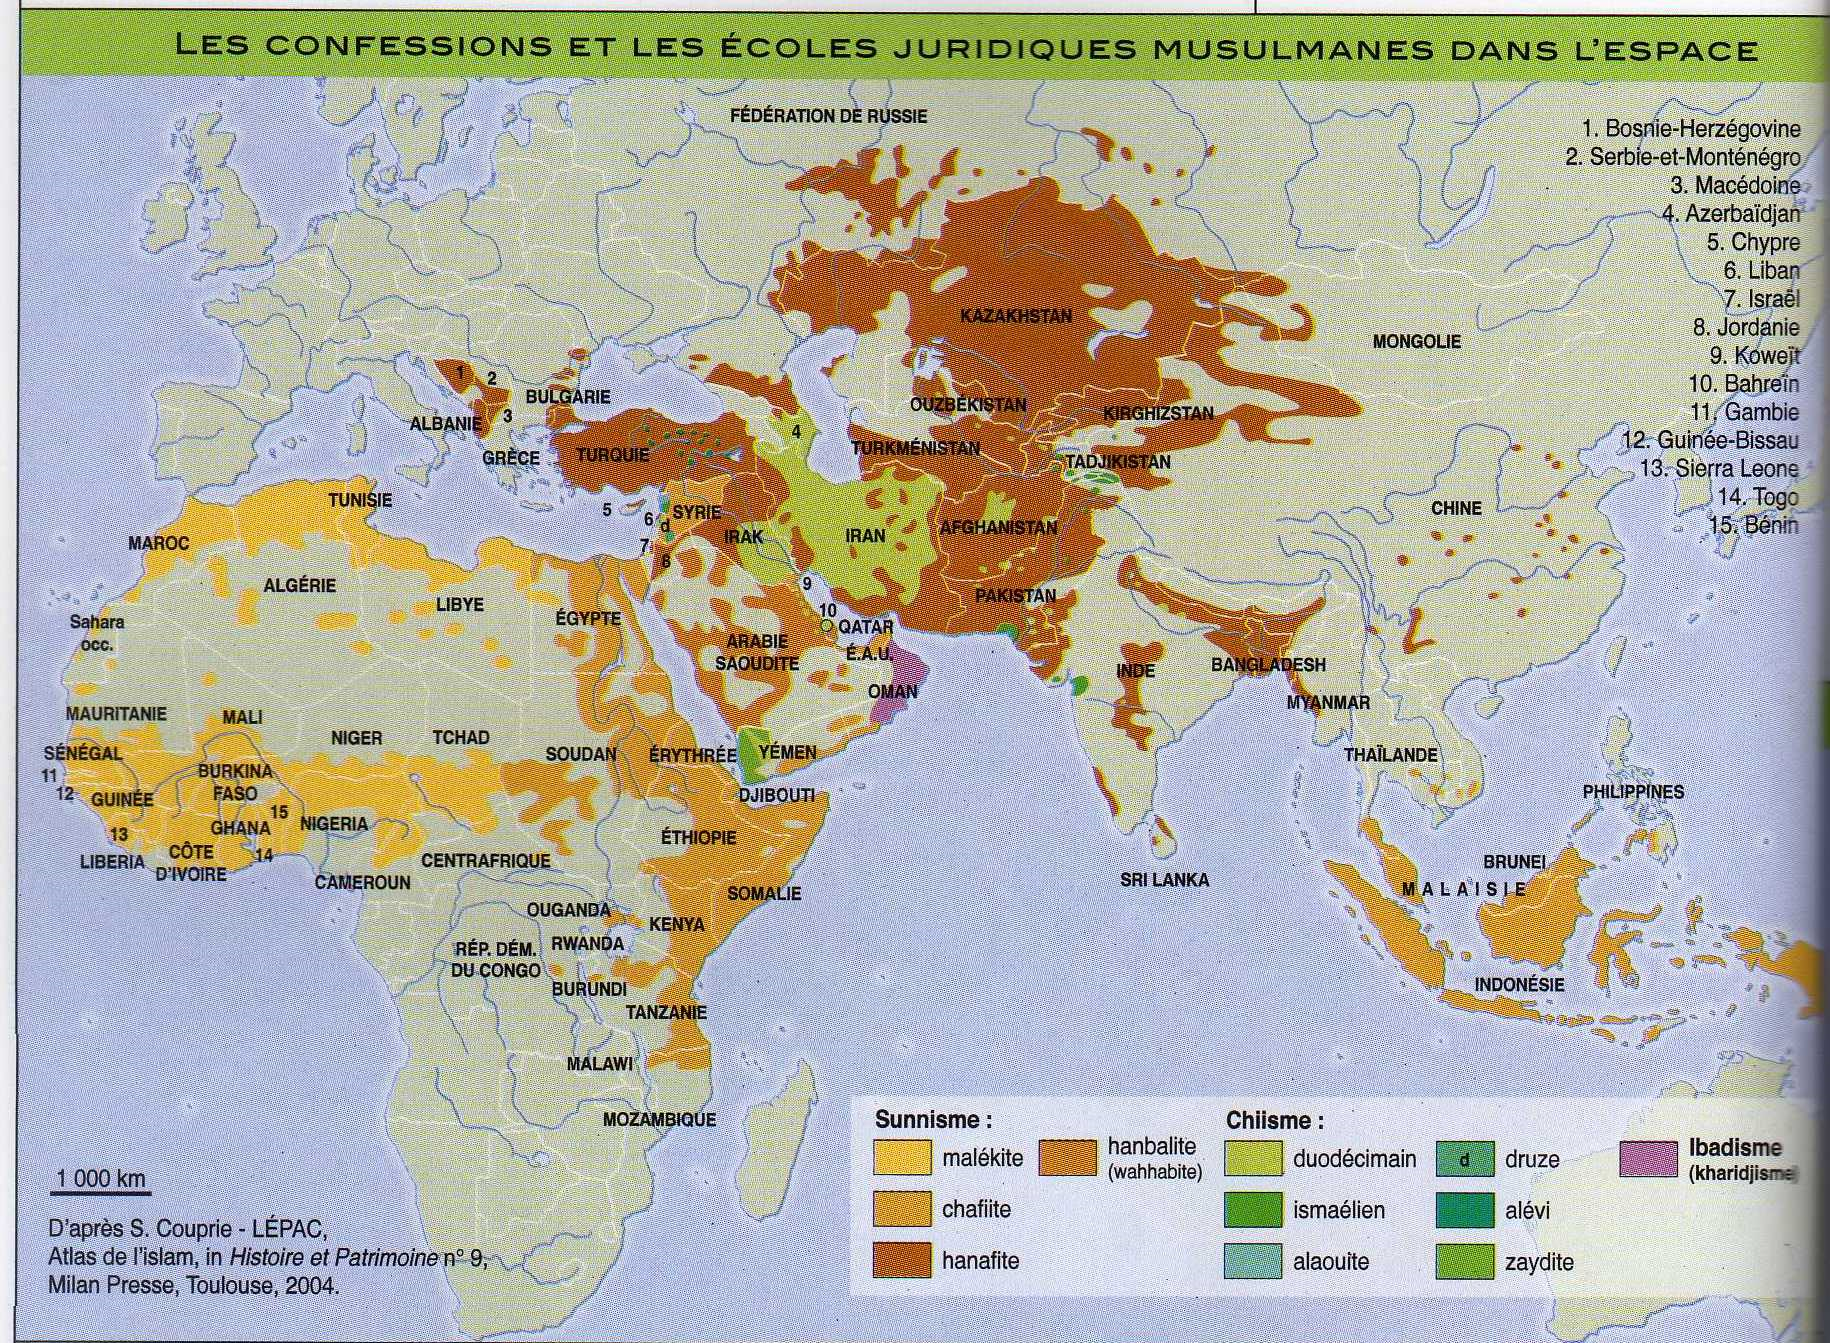
\includegraphics[width=\textwidth]{CourantsIslamContemporain/ImagesCourantsIslamContemporain/CarteSunnisme.png}
 
    \label{fig:my_label}
\end{figure}



\bi 
\item  malékisme : Afrique Nord et ouest.
\item Chafiite : Est de l'Afrique et surtout Egypte 
\item Hanafite : Turquie, asie Centrale, Inde. \textit{les empires turques}
\item Hanbalite : surtout Arabie Saoudite, transformé en \textit{Wahhabisme} au XX, avec une extension au dela de l'Arabie Saoudite en 1960.
\ei 


\subsection{Trois grands courants dans le sh'isme}


\begin{Synthesis}[divergence en Si'isme : les courants]
Des désaccords sur Qui est Imam et sur la \textit{nature de l'Imam}. Il peut être investi de pouvoirs divins.
\end{Synthesis}

\bi 
\item Les duodécimains (ils reconnaissent 12 imams) : les shi'ites Iraniens
\item les Ismaeliens ou septimains (7 imams, l'Aga Khan), Liban.
\item zaydites (5 imams) : Yemen. Au niveau de la doctrine, ils reconnaissent peu de pouvoirs divins aux Imams (proches des Sunnites de ce point de vue).
\ei 
Les Ibadites sont Khajidites. Les druzes et les Alaouites (Alevi en Turc) sont issus du shi'isme (en se proclamant le Maadi) mais ne sont pas considérés comme musulmans par les autres musulmans.  A ne pas confondre à la famille Alaouites au Maroc qui sont tout à fait sunnite (Alaouite veut dire descendant d'Ali). L'Iran reconnait les Alaouites comme shi'ites pour des raisons politiques. 

\subsection{diversité culturelle}
L'islam s'est acculturé aux cultures qu'il a rencontré.
\paragraph{Mosquée}
Le seul élément architectural à une mosquée est la qibla qui indique la Mecque : le Mihrab.

\bi
\item la mosquée bleue a été constituée sur le plan de Sainte Sophie
\item Mosquée de Djenné.
\item La mosquée de Lagos : représente un style baroque brésilien.
\item Xian
\item la grande mosquée de Paris : sur l'image d'une mosquée marocaine
\item Mosquée contemporaine de Créteil

\ei 

\paragraph{L'habit féminin} D'après le Hadith "on ne doit montrer que les mains et le visage". 

\bi
\item les danseuses de cours à Surakarta
\item la burqa, avec grillage sur les yeux, asie centrale et Afghanistan dans certains milieux
\item des vétements de couleur et le shadri, vêtement traditionnel en Asie centrale paysanne voile que l'on met différemment selon qu'on est seul, ...
\item en Afrique, habit d'abord ethnique et non religieux. 
\item En France, les jeunes : le bandeau pour tenir le foulard et le foulard coloré. et certaines ne portent pas le foulard
\ei 

\paragraph{Pourquoi une impression d'uniformisation} La mondialisation crée l'uniformisation et certains courants wahhabites incitent à l'uniformisation sur l'influence saoudite.

\subsection{Observer l'islam}

 
\newlength\q
\setlength\q{\dimexpr .5\textwidth -2\tabcolsep}

\begin{table}[h!]
\sidecaption{\textit{Observer l'Islam} Clifford Geerzt, il a été au Maroc et en Indonésie}
%\begin{tabular}{p[7cm]p[7cm]}
\noindent\begin{tabular}{p{\q}p{\q}}
\toprule
\textbf{Maroc}                                                     & \textbf{Indonésie}                                               \\ 
\midrule
Tribale                                                            & Paysanne                                                         \\
\textit{Audace}                                                    & \textit{Application}                                             \\
une culture préalable moins riche                                  & L'islam est arrivé sur une civilisation hindouiste et bouddhiste \\
Un islam de dévotion aux saints (en particulier le saint guerrier) , austérité morale, pouvoirs magiques, piété agressive & malléable, syncrétique  \\
Uniformisation, facteur de civilisation & diversification, multiforme\\

\bottomrule
\end{tabular}
\end{table}

\subsection{Bibliographie}

\begin{quote}
\textbf{Atlas}

*DUPONT, Anne-Laure \emph{Atlas de l'islam dans le monde}, nouv. éd.,
Autrement, Paris, 2014. GUIDERE, Mathieu \emph{Atlas des pays arabes. De
la révolution aux démocraties}, Autrement, Paris,

2012.
\end{quote}

\hypertarget{ouvrages}{%
\subsection{Ouvrages}\label{ouvrages}}

\begin{quote}
BURESI, Pascal \emph{Géo-histoire de l'islam}, Belin, Paris, 2005.

GEERTZ, Clifford \emph{Observer l'islam : changements religieux au Maroc
et en Indonésie}, La Découverte, Paris, 1992.

*MERVIN, Sabrina \emph{Histoire de l'Islam. Doctrines et Fondements},
nouv. éd., Flammarion, 2016.

DE PLANHOL, Xavier \emph{Les nations du prophète}, \emph{manuel
géographique de politique musulmane}, Fayard, Paris, 1993.
\end{quote}

\chapter{
Le soufisme ou la mystique en islam}


\section{Calligraphie}


\includegraphics[width=\textwidth]{Images/image013.jpg}


« Aux commencements de l'islam, il n'y a ni ascètes ni soufis.
L'ascétisme et la mystique musulmane vont se développer dans les
sociétés de convertis à partir du IX\textsuperscript{e}~siècle. C'est un
phénomène d'hybridation culturelle. Le soufisme est d'abord le fait de
maîtres isolés au IX\textsuperscript{e}~siècle, vivant du côté de
l'actuel Iran. À partir du XII\textsuperscript{e}~siècle se développent
les premières confréries, dont certaines sont encore vivantes
aujourd'hui. Dans l'islam, la mystique est aussi développée que dans le
christianisme, mais elle a été davantage combattue. D'abord par les
juristes, qui voyaient d'un mauvais œil ces croyants qui s'émancipaient
des règles sociales, puis par le wahhabisme, qui les a massacrés dans la
deuxième­ moitié du XVIII\textsuperscript{e}~siècle ».\sn{Jacqueline Chabbi}


« Dans cette calligraphie, j'ai recherché la stabilité mais aussi un
geste plus tendre. Certains y verront peut-être un personnage
agenouillé, en prière\ldots{} Pourquoi pas ? J'offre une image sur
laquelle je ne peux pas toujours mettre des mots. C'est à ceux qui
regardent d'interpréter mes images. Quand je peins, je prends toujours
en considération le blanc laissé par la trace. En calligraphie, un
principe dit :\emph{~``Le noir de votre calligraphie, c'est vous. Le
blanc de votre calligraphie, c'est vous aussi.''}~J'y pense souvent.
Dans les textes anciens, le soufi -- que l'on peut traduire par
``mystique'' -- doit travailler sur soi-même pour retrouver la lumière
intérieure. Il devient alors pur et peut arriver à rencontrer la
divinité. »\sn{Hassan Massoudy}


\section{Introduction}
\paragraph{ Qu'est-ce que le soufisme~?} Pour les soufis, il s'agit de la dimension
spirituelle et originelle de l'islam. Le mot originel est important~: il
signifie que le soufisme est connaturel à l'islam, qu'il est l'islam. Il
ne s'agit pas d'un développement ultérieur qui aurait eu lieu sous
l'influence du monachisme chrétien ou du šī`isme, mais de l'islam vécu
par Muḥammad et ses compagnons. Donc, pour les soufis, Muḥammad est un
soufi. Les salafs, les anciens, les compagnons de Muḥammad sont soufis.
On comprend que si al-Ġazālī \label{theol:AlGazali27} considère le soufisme comme la voie par
excellence pour aller à Dieu, il n'en demeure pas moins que sous sa
plume la référence aux salafs y est importante.
\mn{Le soufisme et Si'isme

\begin{itemize}
\item
  historiquement, plutôt dans l'islam sunnisme
\item
  dans le si'isme, c'est presque intégré tellement il est naturellement
  spirituel.

  \item
    Dans le cadre duodecimain strict, on ne prie pas les imams
  \item
    Mais en fait, il y a des «~sectes~» qui vont le prier, à commencer
    par le fait qu'on va considérer que c'est le «~l'imam caché~»

  \end{itemize}}
Pour autant, cette affirmation d'éminents soufis n'est pas partagée par
l'ensemble des penseurs de l'islam, et au cours de l'histoire, le
soufisme a pu faire l'objet de critiques, de contestations, de
réfutations plus ou moins virulentes. Certaines des pratiques soufies
ont pu être considérées comme hétérodoxes, innovatrices, non conformes à
l'islam des origines. Ce sont ces accusations récurrentes qui permettent
d'expliquer pourquoi on s'en prend aujourd'hui encore à des mosquées
soufies. 
\paragraph{Le wahhabisme est la matrice idéologique anti-soufie
contemporaine}. Comme nous l'avons vu, il est né en Arabie à partir du
18\textsuperscript{ème} siècle en contestant les confréries soufies
jugées non confirmes à l'islam. Aujourd'hui, l'État islamique de l'Irak
et du Levant, au lendemain de la conquête de Mossoul a distribué aux
habitants une charte comprenant 16 commandements~: à l'article 10, il
est écrit que toutes les manifestations publiques contraires à l'islam
sont interdites (article 10). En 2014, quatre sanctuaires sunnites et
soufis et six mosquées chiites ont été détruites dans la province de
Ninive, sous contrôle des insurgés. La destruction la plus spectaculaire
fut celle du tombeau du prophète Jonas -- Yunus en arabe -- qui a été
réduite à un amas de cailloux.

En Égypte, dans le Sinaï, en décembre 2016, un shaykh soufi et un de ses
disciples sont assassinés par le groupe de l'Etat islamique. Le 24
novembre 2017 l'attentat à la mosquée al-Rawdah de Bir al-Abed fait 305
morts -- à cette mosquée était attachée une \emph{zāwiya} -- édifice
religieux fréquenté par des soufis et des conscrits de l'armée. Cette
mosquée soufie appartient à l'ordre soufi des ǧarirites du nom d'Aïd Abū
Ǧarīr qui a fondé trois loges dans le Sinaï au 20\textsuperscript{ème}
siècle dont celle de Bir al-Abed\sn{Sur la sociologie religieuse
  du Sinaï, voir l'article d'Ismaïl Alexandrani~:
   \url{http://orientxxi.info/magazine/-genealogie-du-djihadisme-au-sinai,0687}}.

\vide{i--duxe9finir-le-soufisme}{%
\section{{Définir le soufisme
}}\label{i--duxe9finir-le-soufisme}}

En guise d'apéritif, écoutez la voix d'Henri Corbin (m. 1978),
philosophe et éminent orientaliste français, spécialiste surtout de
l'islam iranien et de la gnose chiite. \emph{Extrait d'un entretien avec
Bernard Maxime Latour en 1971}.

Définition complexe donc, «~tâche scabreuse~»\ldots{} essayons cependant
de le définir à partir de la manière dont les musulmans eux-mêmes
présentent le soufisme, le \emph{tasawwuf} en arabe.

Pour cela, je vous propose de lire un extrait du livre Traité de
Kalābāḏī, \emph{Kitāb al-ta`arruf li-maḏhab ahl al-tasawwuf} qui a été
traduit par Roger Deladrière\sn{~\textsc{Kalābāḏī}, \emph{Kitāb
  al-taʿarruf li-madhhab ahl al-taṣawwuf} {[}traduction française~:
  Traité de soufisme, Les Maîtres et les étapes, traduit de l'arabe et
  présenté par Roger Deladrière, Paris, Actes-Sud, Sinbad, 1981.}.
Kalābāḏī \label{theol:Kalabadi} est un auteur persan, mort aux environs de 990. Cet ouvrage
cherche à réconcilier le soufisme et l'orthodoxie. C'est un classique,
apprécié de tous. En son introduction, il consacre plusieurs pages à
cerner le sens de soufisme par l'étymologie. C'est un peu dense et
technique, mais tout à fait accessible. En ces derniers cours, ce long
extrait vous permet de prendre contact avec un texte fondamental en
islam et avoir la satisfaction d'y être à peu près à l'aise.
\begin{quote}
    

«~Certains ont soutenu que les soufis furent appelés de ce nom à cause
de la pureté (\emph{safā}') de l'intime de leur être et de l'absence de
souillure de leurs actes. Selon Bichr Ibn al-Hârith, «~le soufi est
celui dont le cœur est pur à l'intention de Dieu~». D'après un autre,
«~le soufi est celui dont le comportement est pur à l'égard de Dieu et
dont le charisme (\emph{karâma}) qui lui vient de Dieu -- que soient
proclamées Sa Puissance et Sa Majesté~! -- est pur~».
\end{quote}
Selon une autre explication, les soufis ont été appelés ainsi parce
qu'ils sont, devant Dieu, au premier rang (\emph{saff}), du fait que de
leurs aspirations (\emph{himam}) s'élèvent jusqu'à Lui, que leur cœur se
tourne avec empressement vers Lui, et que l'intime de leur être se tient
en arrêt devant Lui.

D'après certains, ils auraient été désignés du nom de soufis parce que
leurs caractéristiques sont proches de celles des «~hommes du banc~»
(\emph{ahl al-suffa}) qui vivaient à l'époque de l'Envoyé de Dieu -- que
Dieu prie sur lui et le salue !

Selon d'autres, ils furent nommés soufis parce qu'ils portaient un
vêtement de laine (\emph{sûf}).

Ceux qui rattachent leur nom au «~banc~» (\emph{suffa}) et à la
«~laine~» (\emph{sûf}) expriment ainsi l'apparence extérieure de leur
état spirituel. \paragraph{ Ce sont en effet des hommes qui ont délaissé ce bas
monde}, ont quitté leur demeure, ont fui leurs amis, parcourant les pays,
le ventre creux, dénudés, ne prenant des choses d'ici-bas que
l'indispensable pour avoir une tenue décente et calmer leur faim. Parce
qu'ils ont quitté leur demeure on les appelle aussi «~étrangers~»
(\emph{ghurabâ'}), et à cause de leurs nombreux voyages on les désigne
sous le nom de «~pèlerins~» (\emph{sayyâhûn}). Du fait de leurs
pérégrinations dans les régions désertiques et parce qu'ils prennent
refuge en cas de nécessité dans les cavernes, les autochtones les ont
surnommés «~les hommes des cavernes~» (\emph{chikaftiyya}) car le mot
«~\emph{chikaft}~» dans leur langue désigne une grotte ou caverne.

Les Syriens leur ont donné le nom de «~faméliques~» (\emph{jaw'iyya})
parce qu'ils prennent seulement comme nourriture ce qui maintient les
forces dont ils ont besoin, conformément à la parole du Prophète~:
\begin{quote}
"Des aliments qui maintiennent ses forces devraient suffire au fils
d'Adam".~     
\end{quote}
Sarî Saqatî les a décrits en ces termes~: 
\begin{quote}
    «~Ils mangent
comme des malades, ils dorment comme des gens qui font naufrage, et ils
parlent comme des hommes stupides.~»
\end{quote}

Du fait de leur renoncement à la propriété on les a appelés «~pauvres~».
On avait demandé à l'un d'eux ce qu'était le soufi, et il répondit~:
\begin{quote}
   «~Celui qui ne possède pas et n'est pas objet de possession.~» 
\end{quote}
voulant
dire par là qu'il n'était pas l'esclave des désirs. À la même question,
un autre déclara~: 
\begin{quote}
    «~Le soufi est celui qui ne possède rien et qui, si
jamais il vient à posséder quelque chose, le donne.~»
\end{quote}


À cause de leur vêtement et de leur aspect on leur a donné le nom de
soufis, car ils ne portent pas ce qui est doux au toucher et agréable à
regarder, ce qui serait flatter les passions de l'âme, mais uniquement
une tenue décente, se contentant d'un tissu au poil rugueux et d'une
laine grossière.

Tout cela était la condition des «~hommes du banc~», qui vivaient à
l'époque de l'Envoyé de Dieu. Ils étaient en effet «~étrangers~» et
«~pauvres~», des exilés qui avaient quitté leur demeure et leurs biens.
Abû Hurayra et Fadâla Ibn'Ubayd en firent la description suivante~:

\begin{quote}
   «~Ils tombaient de faim à tel point que les Arabes bédouins les
prenaient pour des fous.~» 
\end{quote}
 Ils étaient vêtus de laine, et, au dire de
certains, cela les faisaient transpirer tellement qu'ils exhalaient
l'odeur des moutons qui ont reçu la pluie. Ceci au point que 'Uyayna Ibn
Hisn dit au Prophète~: 
\begin{quote}
   «~L'odeur de ces gens m'incommode, ne
t'incommode-t-elle point toi aussi~?~» 
\end{quote}


La laine est d'ailleurs aussi le vêtement des prophètes (\emph{anbiyā'})
et la mise des saints. C'est ainsi que, selon la parole du Prophète
rapportée par Abû Mûsâ Ach'âri,
\begin{quote}
    «~ soixante-dix prophètes, pieds nus et
vêtus de manteaux de laine, sont passés par le rocher de Rawlâ, et ils
se rendaient au \emph{Temple Antique} (de la Mecque)~».
\end{quote} 

D'après Hasan
Basrî, «~Jésus -- que la paix soit sur lui -- se vêtait de crin, se
nourrissait des fruits des arbres, et passait la nuit là où il
s'arrêtait.~» Selon une autre tradition d'Abû Mûsâ, le Prophète se
vêtait de laine, prenait des ânes comme monture, et se rendait à
l'invitation des pauvres gens. Hasan Basrî disait encore qu'il avait
connu soixante-dix Compagnons ayant combattu à Badr qui ne se vêtaient
que de laine. Ceux qui se comportaient comme les «~hommes du banc~»,
selon ce que nous avons indiqué, ayant les mêmes vêtements et la même
tenue qu'eux, portèrent donc le nom de «~\emph{suffiyya}~» et du
«~\emph{sûfiyya}~» (soufis).

\paragraph{Quand on rattache leur nom à l'élite (\emph{safwa}) et au premier rang
(\emph{saff}), on exprime alors ce qui se rapporte à leur être intime et
à leur état intérieur}. Dieu, en effet, purifie le secret de l'âme et
illumine le cœur de celui qui quitte le monde, y renonce et s'en
détourne. Selon une parole du Prophète,

\begin{quote}
«~quand la lumière pénètre dans
le cœur, il se dilate et s'épanouit.~» On lui demanda «~quel en est donc
le signe, ô Envoyé de Dieu~?~»~; il répondit «~s'éloigner du monde
illusoire, se tourner vers le monde éternel, et se préparer à la mort
avant qu'elle ne survienne.~»    Ainsi le Prophète avait fait savoir que
Dieu illumine le cœur de celui qui s'éloigne de ce bas monde. Et quand
il questionna Hâritha sur la réalité profonde (\emph{haqîqa}) de sa foi
(\emph{imân}), celui-ci déclara~: «~J'ai détaché mon âme de ce monde,
assoiffé pendant le jour, en veillant la nuit, et ce fut comme si je
voyais se dresser le Trône de mon Seigneur, et comme si j'apercevais les
habitants du Paradis qui se rendaient visite et ceux de l'Enfer qui se
repoussaient.~» Selon ce récit, après qu'il se fut détaché du monde,
Dieu lui illumina le cœur, de sorte que ce qui lui était primitivement
caché lui était devenu visible. Le Prophète s'écria alors~: «~Quiconque
veut voir un serviteur dont Dieu a illuminé le cœur n'a qu'à regarder
Hâritha~!~» À cause de ces caractéristiques, de tels hommes ont été
appelés «~illuminés~» (\emph{nûriyya}). Elles étaient également celles
des «~hommes du banc~». Dieu a dit en effet~: «~Il y a là des hommes qui
aiment à se purifier~; et Dieu aime ceux qui se purifient~.~» Il s'agit
de se purifier extérieurement des souillures et de se purifier
intérieurement des pensées qui surgissent dans l'esprit et des idées qui
se meuvent dans la conscience. Dieu a dit~: «~Des hommes que nul négoce
et nul troc ne distraient de l'invocation (\emph{dhikr}) de Dieu.~»
\end{quote}
 

En outre, à cause de la pureté de leur être intime, leur intuition
(\emph{firâsa}) est juste. Selon une tradition du Prophète rapportée par
Abû Umâma Bâhilî~: «~Prenez garde à l'intuition du croyant, car il
regarde avec la lumière de Dieu~!~» Abû Bakr le Véridique avait
déclaré~: «~Mon cœur a reçu l'inspiration que l'enfant porté dans son
sein par Bint Khârija est une fille~»~; et il en fut comme il l'avait
annoncé. De même le Prophète a dit «~La Vérité parle par la bouche de
'Umar.~» Uways Qarâni, salué par Harim Ibn Hayyân, lui rendit ses
salutations en l'appelant par son nom, alors qu'il ne l'avait jamais vu
auparavant~; et il lui dit ensuite~: «~Mon âme a reconnu ton âme.~» «~Si
vous vous entretenez avec les «~hommes de la sincérité (\emph{sidq}),
dit Abû 'Abd'Allâh Antâki, soyez vous-mêmes sincères, car ils sont les
observateurs des cœurs~! Ils pénètrent dans l'intimité de votre âme et
décèlent vos intentions.~»

\paragraph{Quiconque possède de telles qualités~: limpidité de l'être profond,
pureté du cœur, lumière de l'âme, est «~au premier rang~»}, car elles
caractérisent les «~devançants~» (\emph{sâbiqûn}). Selon une tradition
du Prophète~: «~Soixante-dix mille membres de ma Communauté entreront au
Paradis sans Jugement », précisant ensuite «~pour les autres ou pour
eux-mêmes ils n'ont point de recours aux talismans ni aux
cautérisations, mais ils s'en remettent à leur Seigneur avec
confiance.~» À cause de la pureté de leur être intime, de l'ouverture de
leur âme, et de l'illumination de leur cœur, les connaissances qu'ils
tiennent de Dieu sont justes~; ils ne se réfèrent pas aux causes
secondes (\emph{asbâb}), confiants qu'ils sont en Dieu, s'en remettant à
Lui, et acceptant Son Décret (\emph{qadâ}).

Toutes ces qualités et toutes les significations de ces mots se trouvent
réunies dans les noms et les appellatifs désignant la «~communauté
spirituelle~» (\emph{qawm}). Les expressions en sont exactes, et leur
emploi en est facilement compréhensible. Même s'ils diffèrent en
apparence, leur sens est concordant.

\begin{Def}[soufi]
Si on le tire de \emph{safâ'}
(pureté) et \emph{safwa}(élite), le terme qui désigne ces hommes est
alors celui de \emph{safawiyya}. Si on le rapporte à \emph{saff} (rang)
ou \emph{suffa} (banc), ils sont des \emph{saffiyya} ou des
\emph{suffiyya}.
\end{Def}
 Il est possible, dans le premier cas, que la lettre
\emph{wâw} ait été placée avant la lettre \emph{fâ'}, ce qui donne bien
le mot \emph{sûfiyya}(soufis)~; et, dans le deuxième cas, ajouter le
\emph{wâw} à \emph{saffiyya} ou \emph{suffiyya} serait dû à l'usage
linguistique. Si, enfin, on a tiré le mot \emph{sûfiyya} du \emph{sûf}
(laine), il est parfaitement correct, et cette désignation est
linguistiquement juste.

 \paragraph{Ces termes expriment le renoncement et le détachement
de l'âme à l'égard de ce bas monde, le fait de quitter sa demeure et de
voyager sans cesse, de ne pas flatter les passions de l'âme, de purifier
sa conduite, de rendre limpide l'intime de son être, d'ouvrir son cœur,
et de se comporter en «~devançant~». } Ajoutons à cela ce que dit Bundâr
Ibn Husayn~: «~Le soufi est celui que Dieu a choisi pour lui-même et
qu'Il a traité avec affection (\emph{sâfâ}), le libérant de son âme
(égoïste) et lui épargnant dès lors tout effort et toute contrainte en
vue d'un motif personnel. Et le mot \emph{sûfiya~}= il a été traité avec
affection est (un verbe passif) du même type morphologique que
\emph{'ûfiya}~: il a été protégé, à savoir que c'est Dieu qui l'a
protégé, et \emph{kûfiya~}: il a été rétribué, par Dieu, ainsi que
\emph{jûziya~}: il a été récompensé, par Dieu. L'action de Dieu sur lui
est donc manifeste dans son nom même de \emph{sûfî}, et Dieu est seul à
s'occuper de lui.~»

Interrogé sur la définition du soufi, Abû 'Alî Rûdhabâri répondit~:
«~C'est celui qui a revêtu de laine (\emph{sûf}) sa pureté
(\emph{sâfâ}'), qui a fait goûter à ses désirs personnels la saveur de
la privation, et qui, ayant laissé ce bas monde derrière lui, a suivi la
voie de l'Élu (Mohammad).~»

La même question ayant été posée à Sahl Ibn'Abd Allâh Tustarî~: «C'est,
dit-il, celui qui est pur de tout ce qui trouble, qui est rempli de
méditation, qui s'est retiré des hommes pour se consacrer à Dieu, et
pour qui l'or et l'argile se valent.~»

On demanda à Abû-l-Hasan Nûrî ce qu'était le soufisme
(\emph{tasawwuf})~: «~C'est, répondit-il, délaisser tout ce qui flatte
l'âme.~»

Interrogé sur le même sujet, Junayd définit le soufisme~: «~ C'est
purifier son cœur de l'approbation des hommes, abandonner ses tendance
innées, maîtriser les dispositions de la nature humaine, écarter les
incitations égoïstes, fixer en soi les qualités spirituelles, s'attacher
à la connaissance des réalités immatérielles, utiliser ce qui est mieux
pour la vie éternelle, pratiquer le (devoir de) bon conseil envers la
Communauté tout entière, tenir envers Dieu l'engagement de rester fidèle
à la vérité, et suivre l'Envoyé dans (l'accomplissement de la foi).~»

Selon Yûsuf Ibn Husayn~: 
\begin{quote}
    «~Chaque Communauté a une élite, dépôt précieux
de Dieu qu'Il a caché à Ses créatures, et s'il y en a une dans cette
Communauté-ci, ce sont les soufis.~»
\end{quote}

Quelqu'un demanda à Sahl Ibn `Abd Allâh Tustarî~: «~Qui fréquenterai-je
parmi les différents groupes musulmans~?~» «~Tu n'as qu'à fréquenter les
soufis, répondit-il, car rien n'a à leurs yeux une importance exagérée
et ne saurait être totalement désapprouvé. Pour eux, tout acte peut être
interprété, et ils te trouveront des excuses en n'importe quelle
circonstance.~» La même question ayant été posée par Yûsuf Ibn Husayn à
Dhû-l-Nûn~:
\begin{quote}
«~Fréquente, dit-il, celui qui ne possède rien et qui ne désapprouvera
aucune situation dans laquelle tu pourras te trouver, qui ne changera
pas même si toi tu changes beaucoup, car plus tu changeras, plus tu
auras besoin de lui~!~»
\end{quote}
On rapporte également de Dhû-l-Nûn ceci~:
\begin{quote}
    
«~Au bord de la mer, en Syrie,
je vis, dit-il, une femme, et je lui demandai~: «~D'où viens-tu -- que
Dieu te fasse miséricorde~! -- ~?~» Elle me répondit~: «~D'auprès de
gens qui répugnent à reposer leur corps sur une couche, et qui prient
leur Seigneur avec crainte et désir.~» -- Et où vas-tu~? Insistai-je. --
Vers des hommes «~que nul négoce et nul troc ne distraient de
l'invocation de Dieu. -- Décris-les-moi~! Lui demandai-je. Elle se mit
alors à déclamer ces vers~:

\emph{Des hommes dont les préoccupations s'attachent à Dieu, et dont les
aspirations ne s'élèvent vers personne d'autre.}

\emph{Leur quête est celle de leur Maître et de leur Seigneur, et quelle
noble quête que celle de l'Unique, l'Impénétrable~!}

\emph{Ils ne se disputent rien de ce monde, ni rien de ce qui est
excellent, ni nourritures, ni plaisirs, ni progénitures, ni vêtements
somptueux et élégants, ni la joie reposante de rester au pays.}

\emph{Ils ne luttent qu'à la poursuite du lieu éternel dont chaque pas
les rapproche.}

\emph{Ils courent par les étangs et les vallées, et on les rencontre en
nombre sur les hauteurs.}
\end{quote}
\vide{ii--muxe9thode-spirituelle-du-soufisme}{%
\section{Méthode spirituelle du
soufisme}\label{ii--muxe9thode-spirituelle-du-soufisme}}

C'est un itinéraire spirituel qui vise à remonter vers l'être unique, à
quitter la dualité de l'homme, sa duplicité, en vue d'une unification.
Il s'agit d'abandonner la superficialité des choses pour entrer dans la
profondeur de l'intériorité et ne pas être réduit au monde des
apparences.

Dans son \emph{Essai sur le soufisme}, Martin Lings compare le monde à
une pépinière~: tout ce qui s'y trouve a été planté en vue d'être
transplanté ailleurs. La partie centrale de la pépinière est réservée à
des arbres nobles. Ils sont tous en pot et poussent, pas beaucoup, mais
un peu. Mais quand on regarde bien, un des arbres se distingue des
autres. Il est luxurieux, vigoureux, beau. Que s'est-il passé~? La cause
en est invisible. Pour autant, on la devine~: cet arbre a pris racine
dans la terre du jardin à travers le fond de son récipient. Que dit
cette image~? Les arbres sont des âmes et le soufisme est une méthode,
une voie pour prendre racine, pour passer à travers la porte étroite qui
est dans l'âme elle-même et qui débouche sur l'océan de la Divinité. Le
soufi sait qu'il est comme les autres hommes, il sait aussi qu'il est
prisonnier du monde des formes (les pots), mais il sait aussi qu'il est
appelé à la liberté qui l'emporte sur sa captivité.

Le soufisme doit donc permettre de s'enraciner dans l'océan de la
divinité, d'entrer dans la source de la divinité, dans
l'\emph{\underline{origine}} donc. Cette origine est divine,
transcendantale, c'est celle de l'Absolu, de l'Éternel.

\paragraph{Le soufisme est d'abord une méthode~; il est donc un anti-dogmatisme,}
mais il n'est pas sans dogmes. Il ne nie pas le credo musulman, au
contraire~; les soufis ont une profession de foi qu'ils énoncent. Mais
il s'agit de ne pas limiter Dieu à cette profession. Dans cette optique,
le mystique andalou Ibn `Arabī appelle à ne pas se limiter à un credo
particulier. Voici un extrait des \emph{Chatons de la sagesse.} Vous
reconnaîtrez peut-être la voix de Georges Claisse. Dans la suite du
cours, je reviendrai sur cette très grande figure du soufisme.

Voie spirituelle vers Dieu, le soufisme est donc la définition d'une
méthode afin d'atteindre la proximité de Dieu, mais plus encore chez
certains, une union, une unification.

\vide{limitation-du-prophuxe8te}{%
\subsection{L'imitation du
Prophète}\label{limitation-du-prophuxe8te}}

\begin{Def}[Sainteté, suġrā et kubrā]
Le soufisme comme voie initiatique conduisant à la «~proximité divine~»
(\emph{walāya})~distingue selon la sainteté «~mineure~» (\emph{suġrā}),
ouverte à tous les fidèles, et la sainteté «~majeure~» (\emph{kubrā}),
réservée à une élite. 
\end{Def}
Pour parvenir à cette sainteté, la plupart des
soufis invitent à l'imitation du Prophète dans la mesure où il est celui
qui a réalisé cette parfaite proximité. 
\begin{Def}[\emph{nubuwwa}]
prophétie
\end{Def}

Ils posent donc l'existence
d'une relation entre la \emph{walāya} et la \emph{nubuwwa}, la
prophétie, mais si al-Tirmidhī (m. 318/930) accorde à la \emph{walāya}
son autonomie par rapport à la nubuwwa, d'autres au contraire, affirme
qu'il n'est pas possible de s'approcher de Dieu sans la \emph{nubuwwa}. \sn{la question est donc la possibilité de l'usage de la Raison pour accéder à Dieu}

L'hagiographie du Prophète Muḥammad s'est aussi accompagnée d'une
spiritualisation de sa figure~: il est «~l'Homme universel~»
(\emph{al-insān al-kāmil}) qui demeure dans ceux qui l'imitent. Or, la
participation à la «~sainteté prophétique~» permet d'actualiser la
Révélation, autrement dit dans donner les clefs pour chaque époque. Il
s'ensuit un «~Muhammado-centrisme~» car c'est Muḥammad en tant que sceau
des Prophètes qu'il convient d'imiter, de suivre, et donc à qui il faut
obéir. On voit ici que le rapport à la Loi est loin d'être supprimé,
spiritualisé. Au contraire.

 
\subsection{Le souvenir
(\emph{ḏikr})} \label{le-souvenir-dikr}

Le souvenir (\emph{ḏikr}) est au fondement du soufisme.
\begin{Def}[{ḏikr}]
Souvenir,
rappel, invocation, il s'agit de revenir à Dieu, de sortir de l'amnésie
qui guette l'homme, de retrouver le moment où fut scellé le pacte
originel (\emph{mīṯāq}).
\end{Def}
  Cette invocation convient à tout lieu, elle est
la marque d'une adoration continuelle. Le \emph{ḏikr} permet de
retrouver et de vivre de la présence divine.

Le Coran invite à cette évocation, à ce souvenir~: «~Souvenez-vous de
moi et je me souviendrai de vous~» (S. 2, 152). De même, le \emph{ḥadīṯ}
invite à la pratique du \emph{ḏikr}.

Ainsi, par exemple~:

\begin{itemize}
\item
  «~`Les cœurs rouillent comme le fer' dit le Prophète à ses compagnons.
  `Et qu'est-ce qui les fait briller~?' demande l'un d'eux.
  `L'invocation de Dieu et la lecture du Coran'~».
\item
  «~Celui qui invoque son Seigneur et celui qui ne l'invoque pas sont
  comparables l'un à un vivant, l'autre à un mort~».
\end{itemize}

Concrètement, le \emph{ḏikr} consiste à invoquer les noms divins ou à
répéter la première partie de la formule de la \emph{šahāda}~: \emph{lā
ilāha illā Llāh}. Puis, il s'agit de répéter le mot Allāh seul, puis, la
dernière lettre de Allāh, le h\ldots{} dans un seul souffle.

Je vous propose d'écouter {une séance de
\emph{ḏikr}
\url{https://www.youtube.com/watch?v=Xq6bIVtCq14}}\emph{.} 
. Ici, les soufis chantent
ensemble la formule \emph{lā ilāha illā Llāh} sur laquelle se surajoute
une psalmodie. Le rythme s'accélère et indique une forme d'ivresse
spirituelle. Généralement, ces invocations s'accompagnent du balancement
de la tête de gauche à droite et du mouvement des bras.

\url{https://www.youtube.com/watch?v=9BaQunfXPpE}{Ici}, vous avez une
vidéo d'une séance de \emph{ḏikr} dans une confrérie.

\vide{luxe9coute-de-luxe9cho-du-verbe-divin-samux101}{%
\subsection{L'écoute de l'écho du verbe divin
(samā`)}\label{luxe9coute-de-luxe9cho-du-verbe-divin-samux101}}

\begin{Def}[{samā`}]
Le \emph{samā`}, tout comme le \emph{ḏikr} a pour objectif de
réactualiser le Pacte originel. Il s'agit d'écouter la musique comme un
écho de ce pacte scellé. 
\end{Def}
Par la musique, l'écoutant libère son âme pour
trouver Dieu. Il y a une quête d'extase~: c'est le \emph{tawāǧud}. La
fin recherchée n'est pas la musique, mais l'écoute, la musique n'étant
qu'un support pour entendre la parole divine. L'écoute est donc
éminemment spirituelle~mais l'usage de la musique peut être dévoyé et
tombé dans le divertissement. Le soufisme n'est pas en soi favorable à
l'écoute de la musique mais il ne refuse pas usage à des fins
spirituelles. Al-Ġazālī  \label{theol:AlGazali28} considère que le samā` n'est pas en soi licite
ou illicite, et que tout dépend de l'intention (\emph{niyya}) de
l'écoutant. Pour rendre compte de cette ambivalence, le soufi al-Šiblī
(m. 946), connu pour ses excentricités paradoxales, dit du \emph{samā`}
qu'il est 
\begin{quote}
    «~en apparence une source de trouble, mais qu'il recèle un
grand enseignement spirituel (
\TArabe{
السماع ظاهره فتنة، و باطنه عبرة
})
~».
\end{quote}

L'histoire du \emph{samā`} montre qu'il a été associé à la danse, et
qu'il a été aussi assimilé au \emph{ḏikr}.

Ultime remarque~: le \emph{samā`} est une voie, une méthode soufie, mais
il n'est pas reconnu par tous les soufis et bien des maîtres ont aussi
privilégié le silence absolu tels Ibn `Arabi ou les premiers maîtres
šāḏilis.

\vide{la-repentance-tawba}{%
\subsection{{La repentance
(\emph{tawba})}}\label{la-repentance-tawba}}

Le repentir consiste à regretter son péché. Les soufis insistent sur
l'importance des larmes.

Elles sont aussi pleines de signification~: la larme est la goutte qui
s'efface en s'évaporant, après avoir témoigné. Sa disparition est
littéralement une extinction (\emph{fanā'}). Elle est symbole
d'intercession et de transformation\sn{On retrouve chez les
  Aztèques ce symbolisme~: les larmes des enfants que l'on apporte au
  sacrifice étaient dites annonciatrices de la pluie à venir. De même
  les lamentations sont mises en relation avec la miséricorde divine et
  la descente de la manne céleste.}.

Dans le soufisme, les pleurs symbolisent la quête du soufi de vouloir
s'abreuver à la source divine elle-même, de faire descendre la grâce, de
réaliser ainsi la présence divine. Les larmes ne sont pas négatives,
mais elles sont signe d'une espérance, de la promesse d'une joie à
venir. Elles ne sont pas la manifestation d'une séparation d'avec Dieu,
mais surtout un appel à retrouver Dieu, à s'unir à lui.

\vide{la-retraite-spirituelle-ux1e2balwux101}{%
\subsection{{La retraite spirituelle
(\emph{ḫalwā})}}\label{la-retraite-spirituelle-ux1e2balwux101}}

La retraite spirituelle constituait à l'époque antique un «~exercice
spirituel~». Le texte apocryphe intitulé \emph{La théologie d'Aristote}
écrit très vraisemblablement en syriaque au VI\textsuperscript{ème}
siècle et qui est un commentaire (\emph{tafsīr}) de certains passages
des \emph{Ennéades} de Plotin\sn{Pierre Thiellet, «~Notes sur la
  Théologie d'Aristote~» dans Prophyre, \emph{La vie de Plotin}, II,
  Paris, Vrin, 2000, p. 625-638.}, donne pour définition de l'extase le
fait d'être seul avec son âme (\emph{khalawtu bi-nafsi})\sn{Plotin,
  \emph{Ennéades}, IV, 8, 1.}. Il exerça très probablement une influence
dans la théorisation de cette solitude spirituelle. La pratique de la
retraite dans le soufisme renvoie à celle du monachisme chrétien avec
les Pères du désert, où l'éloignement de la ville et de la société était
considéré comme un chemin vers Dieu et un des fondements de l'ascétisme
(\emph{zuhd}). Depuis la \emph{Risāla} d'Abū al-Qāsim al-Qušayrī
(986-1072), toutes les présentations du soufisme intègrent un chapitre
sur les retraites spirituelles, qu'elles soient permanentes ou
périodiques. On appelait ces retraites des «~quarantaines~»
(\emph{arba`īniyya}). Elles étaient comprises comme une \emph{imitatio
prophetae}, à la suite de la retraite de quarante jours de Moïse sur le
mont Sinaï ou de celle de David pour réparer sa faute ou encore bien sûr
de Muḥammad qui allait une fois par an se recueillir (\emph{tahannuṯ})
sur le Mont Ḥirā'\sn{Paul B. Fenton, «~La pratique de la retraite
  spirituelle~», dans Giuseppe Cecere, Mireille Loubet, Samuela Pagani,
  \emph{Les mystiques juives, chrétiennes et musulmanes dans l'Égypte
  médiévale (VII\textsuperscript{e}-XVI\textsuperscript{e} siècles).}
  Interculturalités et contextes historiques, Le Caire, IFAO, 2013, p.
  211-252.}. Vous vous souvenez, c'est pendant un temps de retraite
qu'il reçut la révélation du Coran.

Au livre seizième de l'\emph{Iḥyā'} sur la retraite et la vie retirée
(\emph{`uzla}), al-Ġazālī \label{theol:AlGazali29} indique l'existence d'un débat au sein de la
deuxième génération des musulmans~: certains recommandaient en effet
l'amitié, l'assistance entre les croyants, la fraternité, tandis que
d'autres soulignaient l'importance de l'isolement et de la retraite
spirituelle. «~Fuis les gens comme si tu fuyais le lion~»\sn{\textsc{Al-Ġazālī },
  \emph{Iḥyā' `ulūm al-dīn, op. cit.,} K. 16 (\emph{Kitāb ādāb
  al-`uzla}), B.1, p. 665 {[}V.4, p. 248{]}.} conseille Dawūd al-Ta'i.
On raconte aussi cette histoire à propos de Sahl Ibn al-Ṭustarī (m.
896), grand maître soufi~\sn{\emph{Ibid}., p.666 {[}V.4, p. 251-252{]}}.:
\begin{quote}
    
«~Alors qu'un homme s'avança et lui dit qu'il
voulait lui tenir compagnie, Sahl lui répondit~: `Et si l'un de nous
deux vient à mourir, qui sera le compagnon de l'autre~?' L'homme lui
dit~: `Dieu'. Sahl reprit la parole~: `Qu'il lui tienne donc dès à
présent compagnie'~»
\end{quote}

Mais cette approche spirituelle de la retraite et de la solitude dans la
prière et l'isolement a aussi ses détracteurs. En opposition, on
rapporte les paroles du Prophète Muḥammad~où l'on retrouve le bestiaire
du désert~:

\begin{quote}
«~Satan est un chacal pour l'homme. Comme le chacal il saisit du
troupeau la bête égarée qui s'en est éloignée. Prenez garde aux vallées
et restez attachés aux communautés, aux groupes et aux mosquées~».
\end{quote}

Plus rédhibitoire, ce propos du Prophète de l'islam~\sn{\emph{Ibid}, B.1, ḏ.1, p. 667 {[}V.4, p.
  253-254{]}.}: 
\begin{quote}
   «~celui qui se
sépare du groupe (\emph{ğamā`a}), ne serait-ce que d'un empan, ôte de
son cou l'attache de l'islam » ou encore «~celui qui se sépare du groupe
et meurt mourra en homme de l'époque de l'ignorance
(\emph{ğāhiliyya})~». 
\end{quote}

\paragraph{Quels sont les bienfaits attendus de l'isolement~?}
La retraite permet de se consacrer à l'adoration, à la méditation en se
mettant en confidences intimes (\emph{munāğāt}) avec Dieu, en
privilégiant donc l'intimité avec Dieu plutôt qu'avec une créature.

La retraite permet aussi de se débarrasser des péchés auxquels on
s'expose en fréquentant les gens~: la calomnie, la médisance, la
bigoterie, la duplicité, l'avidité, l'attachement au bas-monde.
Al-Ġazālī \label{theol:AlGazali30} indique que l'habitude des gens consiste à se rincer la bouche
avec l'honneur des gens. La fréquentation conduit à s'accorder avec eux
et à s'exposer à la colère de Dieu. Garder le silence revient à
s'associer à leur médisance car l'auditeur est un médisant. Les récuser,
c'est s'exposer à se faire détester et susciter médisance et calomnie
contre soi, donc la médisance en est redoublée\ldots{}\sn{\textsc{Al-Ġazālī },
  \emph{Iḥyā' `ulūm al-dīn}, \emph{op. cit.,} K. 16, B.2, p. 673 {[}V.4,
  p. 272{]}~}.

La fréquentation des gens nous fait poser des questions vides et
hypocrites. Ainsi quand on voit quelqu'un, on lui demande «~comment ça
va~?~», mais on n'accorde aucune importance à la réponse. L'intérêt que
l'on porte à l'autre dans cette question est faux. Autrement dit, la
fréquentation des gens nous pousse à la duplicité. Al-Ġazālī \label{theol:AlGazali11} voit dans
cette question une innovation blâmable.

Finalement, le critère qui permet de vérifier si la retraite est
\emph{ḥarām} ou \emph{ḥalāl} est celui du bien que l'on retire de
l'autre~de par son beau caractère : «~si tu trouves un convive
(\emph{ğalīs}) qui te rappelle l'image et la conduite de Dieu, alors
attache-toi à lui\ldots{} car c'est là le trésor de l'homme doué de
raison (\emph{ġanīmat al-`āqil})~et le dessein du croyant (\emph{ḍāllat
al-mu'min}) »\sn{\textsc{Al-Ġazālī }, \emph{Iḥyā' `ulūm
  al-dīn}, \emph{op. cit.,} K. 16, B.2, fa.2, p. 677 {[}V.4, p. 285{]}~}.

Troisième bienfait~: celui de l'esprit de querelle et du fanatisme. On
rapporte ce dit de Muḥammad~:
\begin{quote}
    «~Il y aura une époque où pour préserver
sa religion, il faudra fuir de village en village, du sommet d'une
montagne à un autre, d'une pierre à une autre, comme un renard qui
s'échappe. Ce jour-là arrivera quand on ne gagnera sa vie qu'en
commettant des péchés et en désobéissant à Dieu. Alors, à cette époque,
le célibat (\emph{`uzūba}) deviendra licite~»\sn{\textsc{Al-Ġazālī },
  \emph{Iḥyā' `ulūm al-dīn}, \emph{op. cit.,} K.16, B.2, fa.3, p. 677
  {[}V.4, p. 286{]}.}.
\end{quote}

Cependant, al-Ġazālī est le théoricien soufi du juste milieu. Et il
souligne combien vivre en dehors de la communauté peut être l'occasion
de s'enorgueillir. Ainsi, en est-il de cette histoire juive~:

\begin{quote}
«~Un sage {[}parmi les israélites{]} avait rédigé trois cent soixante
opuscules sur la sagesse, si bien qu'il en était venu à penser qu'il
avait été gratifié d'un degré élevé auprès de Dieu. Dieu révéla à son
prophète~: `Va lui dire qu'il a rempli la terre d'hypocrisie et que je
n'agrée en rien son hypocrisie'. Le sage abandonna alors
{[}l'écriture{]} et se retira dans un tunnel sous terre. Il se dit en
lui-même~: `À présent, j'ai atteint le contentement de mon Seigneur.
Mais Dieu révéla à son prophète la parole suivante~: `Dis-lui qu'il
n'obtiendra mon contentement qu'après avoir fréquenté les gens et
supporté leur nuisance'. Le sage quitta son refuge et entra dans les
marchés pour fréquenter les gens, s'asseoir avec eux, partager leurs
repas, déambuler dans les marchés. Dieu révéla alors à son prophète~:
`Maintenant, il a obtenu mon contentement~»\sn{\textsc{Al-Ġazālī },
  \emph{Iḥyā' `ulūm al-dīn}, \emph{op. cit.,} K. 16, B.2, p. 687 {[}V.4,
  p. 312{]}.}.
\end{quote}

Si le soufi doit se retirer dans une cellule en solitude, si c'est là
qu'il se souvient de Dieu, l'enjeu est de parvenir à un état permanent
de retraite intérieure. La démarche se retrouve chez Muḥammad.

Le šayḫ al-`Alawī, soufi algérien qui appartient à la branche
confrérique Šaḏiliya qui a pris naissance au 14\textsuperscript{ème}
siècle et qui met l'accent sur l'invocation du nom de Dieu, a fondé sa
propre confrérie. Sa méthode bien qu'elle s'inscrive pleinement dans
l'esprit de la Šaḏiliya, est aussi originale~:

\begin{quote}
«~La khalwah est une cellule dans laquelle je place le novice après
qu'il a juré de ne pas la quitter pendant quarante jours si besoin est.
Dans cet oratoire, il ne doit rien faire d'autre que répéter
continuellement le nom divin (Allâh) en prolongeant à chaque invocation
la syllabe âh jusqu'à ce qu'il soit à bout de souffle.\\
Préalablement, il doit avoir récité la \emph{shahâdah} (\emph{lâ ilâha
illa Llâh}, « il n'y a de Dieu que Dieu ») soixante-quinze mille fois.

Durant sa retraite, il jeûne rigoureusement tout le jour, ne rompant son
jeûne qu'entre le coucher du soleil et l'aube\ldots{} quelques foqarā'
(mystiques) obtiennent l'illumination soudaine au bout de quelques
minutes, d'autres seulement après plusieurs semaines. Je connais un
\emph{faqîr} qui a attendu huit mois. Chaque matin, il me disait: « Mon
cœur est encore trop dur », et il poursuivait sa ḫalwā. À la fin, ses
efforts furent récompensés. »\sn{Martin Lings, \emph{Un saint
  musulman}, p. 96.}
\end{quote}

\vide{station-maqam-et-uxe9tat-ux1e25ux101l-spirituel}{%
\subsection{{ Station (\emph{maqam}) et état
(\emph{ḥāl}) spirituel
}}\label{station-maqam-et-uxe9tat-ux1e25ux101l-spirituel}}

Il existe dans le soufisme une théorie des états et des stations
spirituelles qui dessinent le cheminement et la progression du soufi.
\begin{Def}[\emph{maqam} (station)]
représente dans l'itinéraire vers Dieu, un
degré de perfection spirituelle obtenu à la suite de l'effort personnel
du mystique.
\end{Def}

 Le \emph{ḥāl} (état) en revanche consiste en une
disposition que l'on ne doit qu'à Dieu: «~Les états, disait Al Qushayrī,
sont des dons, les stations sont des mérites~».
\begin{Def}[\emph{ḥāl}]
Le \emph{ḥāl} est fondamentalement un état passager, éphémère. Le but du
soufi est de transformer le \emph{ḥāl} en état permanent (\emph{maqām}).

\end{Def}
Il faut passer du conjoncturel au structurel. Ainsi, la crainte peut
saisir le croyant à la lecture d'un passage du coran, suite à la
rencontre avec un savant ou un soufi\ldots{} mais cette crainte
ressentie doit habiter le croyant au-delà d'une sensation. Le combat
consiste donc à rendre permanent le \emph{ḥāl}.

\vide{iii--grandes-figures-soufies}{%
\section{{Grandes figures soufies
}}\label{iii--grandes-figures-soufies}}

\vide{ux1e25asan-al-baux1e63rux12b-643-728}{%
\subsection{Ḥasan al-Baṣrī
(643-728)}\label{ux1e25asan-al-baux1e63rux12b-643-728}}

Il est, selon les historiens arabes, le premier soufi. Il semble
cependant avoir été plus ascète que mystique~: il recommandait le mépris
du monde, l'examen de conscience. Pour lui, les spirituels se
reconnaissent à leur désir de Dieu. Il faut savoir se taire~: car parler
rajoute quelque chose à l'absolue transcendance de Dieu et finit par
l'offenser.

Ḥasān al-Basrī n'emploie pas le mot \emph{ḥubb} (amour réciproque). Il
dit~: 
\begin{quote}
    comment je peux dire que Dieu a un amour pour moi~?
\end{quote}
 Il préfère
donc le mot \emph{`išq}~: c'est l'éros, le désir. Mais ce mot ne se
trouve pas dans le Coran. Et le théologien hanbalite al-Ansarī le
refuse. Il y voit une intrusion de la raison humaine. Un bel exemple de
pluralisme en islam sur la question de l'amour de Dieu.

À noter que si le salafisme-wahhabiste combat le soufisme, les
salafistes reconnaissent à Ḥasan al-Baṣrī une autorité en tant
que~transmetteur de nombreux \emph{ḥadīṯs}.

\vide{rux101bia-m.-185801}{%
\subsection{{Rābi`a (m. 185/801)
}{3.2 Rābi`a (m. 185/801) }}\label{rux101bia-m.-185801}}

Elle est la première femme mystique de l'islam, la première soufie, un
premier témoin avec Ḥasan al-Basrī. Elle est née 60 ans après la mort du
Prophète Muḥammad. Il y a deux dates pour sa mort, la première la fait
mourir au milieu du huitième siècle à 55 ans, la seconde à la fin du
huitième siècle à 90 ans. Elle a initié la science de l'amour \emph{`ilm
al-maḥabba.}

Rābi`a n'est pas un prénom, cela veut dire la quatrième~: son milieu
familial était très pauvre et comme elle est la quatrième à être née,
son père l'a appelée La Quatrième. On sait peu de choses sur sa vie de
jeune femme. Fut-elle flûtiste~? prostituée~? Certains biographes le
suggèrent donnant au personnage une plus grande renommée.

Dans l'histoire de la pensée, elle est citée par les grands théologiens.
Ainsi, par exemple, Ğāḥiẓ (m. 867) parle d'elle dans le \emph{Livre des
animaux}. Il rapporte le propos de Rābi`a alors qu'on lui offrait un
esclave pour la servir et elle s'y opposait~: «~J'aurais honte de
demander des biens de ce monde à Celui à qui ils appartiennent ; comment
dès lors les solliciterais-je de gens à qui ils n'appartiennent pas ?~».

Ǧāḥiẓ a souligné la qualité rhétorique du propos (il est spécialiste de
rhétorique) ; il y reconnaît en arabe une éloquence exceptionnelle, une
prouesse rhétorique, mais aussi
une preuve ontologique contre l'esclavage.

Un exemple très connu est celui des deux seaux d'eau~ et des charbons~:
Ici, vous allez entendre la voix de Salah Stétié, un écrivain libanais
qui a traduit dans un français remarquable ses plus beaux poèmes.


\subsection{Pour aller plus loin~: les femmes soufies}

Sulaymī consacre un petit opuscule intitulé \emph{Les femmes soufies},
seconde moitié du 10\textsuperscript{ème} siècle, après le traumatisme
de Ḥallāğ \\


Quelques paroles «~insolentes~»~ (l'expression et de Salah Stétié)

\emph{Sur le paradis}

«~Un jour on récitait devant elle ce verset du Coran~: `Ce jour-là, la
seule occupation des hôtes du paradis sera de se réjouir en compagnie de
leurs épouses, ils se tiendront sous des ombrages, accoudés sur des lits
d'apparat'. Elle dit~: `pauvres gens du paradis, les voilà bien occupés
de leurs femmes~!'~»

\emph{Sur le Prophète}~

«~Aimes-tu le prophète~? Certes je l'aime, mais l'amour du créateur m'a
détourné définitivement de l'amour de toute créature~»

\emph{Sur les deux amours}

\begin{quote}
Je t'aime de deux amours

Amour de mon bonheur et amour digne de toi

Quant à cet amour de mon bonheur

c'est que je m'occupe à ne penser qu'à toi seul

à l'exclusion de tout autre

Et quant à cet autre amour dont tu es digne

C'est mon désir

Que tes voiles tombent et que je te voie

Nulle gloire en moi en l'un en l'autre,

non mais louange à toi pour celui-ci comme pour celui-là\sn{Traduction
  Salah Statié, \emph{Rabi'a de feu et de larmes,} Fata Morgana, 2010.}.
\end{quote}

\emph{Sur le pardon}

«~On lui demande~: `J'ai commis de nombreux péchés, Dieu me
pardonnera-t-il si je me repens~?' Elle répond~: il faut que Dieu te
pardonne d'abord et ensuite tu te repentiras~».

\begin{quote}
Ma coupe, mon vin, mon hôte, sont trois,\\
Et moi que remplit l'amour : je suis la Rabi'a\\
Celui qui verse le vin fait circuler sans cesse\\
la coupe de la volupté et du luxe\\
Si de mes yeux je vois, je ne vois que pour Lui,\\
Si regardée je suis, je suis vue avec Lui.\\
O ! Toi qui me blâmes ! Sa beauté oui, je l'aime~!\\
et par Dieu, mes oreilles n'ont que faire de Ton blâme.\\
Que de nuits délirantes j'ai passées, feu, tourment,\\
et mes yeux se sont fait sources par mes larmes !\\
et aucune de mes larmes n'a pu remonter à sa source\\
mon union avec Lui n'a pas duré.\\
blessé, meurtri, mon œil plus jamais ne s'apaise
\end{quote}

\vide{al-hallux101ux11f-m.-309-922}{%
\subsection{al-Hallāğ (m. 309 /
922)}\label{al-hallux101ux11f-m.-309-922}}

C'est un personnage complexe dont l'évolution religieuse a fait couler
beaucoup d'encre. Louis Massignon lui a consacré sa thèse doctorale.
C'est un mystique musulman, crucifié, criant du haut de sa croix~: «~Je
suis Dieu~»\ldots{} expression de sa doctrine de l'unification
(\emph{ḥulūl}).

Son nom lui vient du métier de son père~qui était cardeur de coton. Ses
disciples l'appelaient \emph{al-Hallâj al-asrâr} c'est-à-dire le cardeur
des pensées secrètes. Il voulait dévoiler les «~secrets de l'union
divine~» (\emph{asrār al-tawḥīd})\sn{Pour sa biographie, je
  m'appuie notamment sur l'introduction de Stéphane Ruspoli : \emph{Le
  Message de Hallâj l'Expatrié}, Collection Patrimoine Islam, Paris,
  Cerf, 2006.}.

Quelles relations entretenait-il avec le calife Mu'tadid (892-902) puis
le calife Muqtadir (m. 932) qui le laissa exécuter~? Quels furent ses
contacts avec le christianisme~? Dans quelle mesure trouva-t-il dans la
figure du Christ et de sa Passion un modèle, alors même que l'islam
réfute la mort sur la Croix de Jésus~? Dans quelle mesure ses voyages au
Cachemire lui ont-ils permis de s'imprégner de la sagesse hindoue~?

Il passera une année entière de retraite à La Mecque, imitant ainsi les
retraites solitaires de Muhammad sur le mont Hira. C'est un prédicateur,
un enseignant. Pour lui, l'islam «~n'est pas seulement la soumission
passive~» devant Dieu, ni l'obéissance aux rites prescrits, mais une
doctrine du salut, de la connaissance, de l'amour~». Il était partisan
de la voie du blâme, et assumait ses provocations. Il disait~ainsi :
«~La mécréance et la foi se distinguent seulement par leur nom, mais en
réalité il n'y a pas de différence entre les deux~». En 902, suite à une
expérience spirituelle très forte, il a la révélation du Nom Suprême de
Dieu. Cette révélation fut à la base d'une profonde mutation. Il résume
sa quête en une formule~: «~Anâ al-Haqq~» - littéralement «~je suis le
Vrai~», je suis Dieu.

 
\paragraph{Ibn Atā}\label{ibn-atux101}

Il est dénoncé comme agitateur politique, accusé de comploter contre la
sûreté de l'État et de tenir des propos hérétiques, blasphématoires. Il
est arrêté en 913. Il comparaît devant le vizir Alî ibn `Îsâ qui le
jugea après interrogation «~complètement ignorant du Coran et des
sciences annexes, droit canonique (\emph{fiqh}), Tradition
(\emph{Sunna}), poésie et philosophie arabe~»\sn{Stéphane Ruspoli,
  \emph{op. cit}. p. 34.}. «~On croit rêver~»~! Ibn Atā convoqué au
tribunal déclara Hallāǧ innocent des charges dont on l'accusait et
déclara sa profession de foi totalement valide. Fou de rage, le ministre
le fit battre et Ibn Atā mourut une semaine plus tard.

Hallāǧ arrive au supplice. Il a 65 ans. Il récite encore quelques vers
du Dîwân. Il fait sa prière sous les yeux de ses compagnons en disant~:
«~Ne vous inquiétez pas de cette affaire, car je reviendrai parmi vous
après trente jours~». Il est crucifié. La forme de la crucifixion dans
sa forme musulmane vient des Perses sassanides qui la pratiquaient
couramment. Elle est plus violente, brutale, spectaculaire que la
crucifixion romaine. Sa prière avant de mourir est marquée par la
compassion et la résignation.

Son biographe Stéphane Ruspoli commente~: «~On aura appliqué à la lettre
contre un des plus grands saints musulmans qui lutta pacifiquement pour
la cause de l'islam et la gloire de Dieu, ce verset sombre du Qoran~:
«~Ceux qui combattent Dieu et son Envoyé, et qui sèment la corruption
sur la terre, leur rétribution sera d'être tués, ou crucifiés~; qu'on
leur tranche les mains et les pieds, ou bien qu'on les bannisse du
territoire. Ce sera leur sanction ici-bas, tandis qu'un grand châtiment
les attend dans l'autre monde~» (5, 33)~» (p.35).

Quelques extraits de ses poèmes

\emph{\textbf{Kâna li qablî ahwâ (p. 101)}}

\begin{quote}
\emph{J'ai abandonné aux gens leur usage et leur religion}

\emph{pour me dédier à ton amour, toi ma religion et mon usage.}
\end{quote}

\emph{\textbf{Al-`ayn tubsiru (p. 102)}}

L'œil aperçoit Celui qu'il aime et puis le perd de vue,

Mais le regard du cœur ne cesse jamais de le contempler.

Quand Il n'est pas avec moi, son souvenir m'accompagne,

et le cœur le voit toujours, bien qu'Il se dérobe à mon œil.

\emph{\textbf{Tala'at as-shams (p. 109).}}

\begin{quote}
Le soleil de Celui que j'aime s'est levé de nuit,

Il a brillé sans plus connaître de couchers.

Le soleil du jour se couche certes la nuit,

Mais le soleil des cœurs ne saurait se coucher.

Celui qui aime le Bien-Aimé vole vers Lui,

si grand est son désir d'aller à sa rencontre.
\end{quote}

\emph{\textbf{Li'l `ilm ahl (p. 128)}}

\begin{quote}
Je suis un orphelin, et pourtant j'ai un Père que j'invoque.

Mon cœur tant que je vis s'afflige de son absence.
\end{quote}

Remarquez qu'il s'adresse ici à Dieu avec le nom de Père.

\emph{\textbf{Anâ man ahwâ (p. 129)}}

\begin{quote}
Je suis devenu Celui que j'aime et Celui que j'aime est devenu moi

Nous sommes deux esprits habitant en un même corps.
\end{quote}

\emph{\textbf{Tafakkartu (p. 153)}}

\begin{quote}
j'ai longuement réfléchi aux diverses religions en tâchant de les
assimiler,

puis je les ai ramenées à un seul Fondement ayant maintes ramifications.

Ne demandez pas à un seul homme de s'en tenir à un culte déterminé,

car cela l'écarterait certainement du Fondement divin assuré.

Ce qu'il réclame, c'est un Fondement lui permettant d'élucider

les nobles idéaux et les hautes conceptions afin de les réaliser.
\end{quote}

\emph{Commentaire~}: Ici, l'universalisme religieux de Hallâj semble
accepter tous les cultes, sachant que tout vient de Dieu qu'il est la
sève, l'essence, le Fondement (\emph{al-asl}) qui se transmet aux
ramification de la foi (\emph{shu'ab al-îmân}).

\vide{ibn-arabux12b-m.-1240}{%
\subsection{Ibn `Arabī (m. 1240)}\label{ibn-arabux12b-m.-1240}}

C'est un maître soufi. Incontournable. Pour lui, la pensée de Hallāǧ
accuse une certaine dualité au moment de l'union qui se trouve résolue
dans l'unification. Sur ce point, Ibn `Arabī lui reproche d'avoir laissé
survivre cette dualité dans l'expérience de l'union. Pour lui, l'homme
n'est plus une négation pure qui montre et démontre la puissance de
l'affirmation de l'un, mais par son existence nécessaire, il est l'image
de son créateur, il le représente.

La création est le néant par essence. Elle est illusoire. Elle ne sera
jamais le réel éternel~: «~Tu prétends qu'un autre qu'Allah puisse jouir
de l'Existence~: c'est le nier, et tu es formellement coupable
d'idolâtrie~». (cf. Léo Schaya, \emph{La doctrine soufique}, p 30).

Dieu est au-delà de la dualité de l'être et du non-être. On ne peut pas
justifier l'existence de la dualité entre Lui et un autre que lui. Il
rejette la distinction entre cause et effet. Tout ce qu'il a créé est
une manifestation de lui.

Le maître a influencé des confréries (\emph{turuq}) notamment la
Ḫalwatiyya. Il représente la tradition savante du soufisme. Pourquoi~?

C'est complexe. Mais il existe des facteurs explicatifs. Ainsi, Ibn
`Arabī aurait prédit la victoire des Ottomans et la conquête de la
Syrie. Il s'ensuit que la dynastie lui a accordé un patronage.

Mais plus sérieusement, l'évolution du soufisme au
13\textsuperscript{ème} siècle, le développement des confréries ont créé
un appel d'air doctrinal. Les fondateurs de ces branches confrériques
que sont al-Jîlânî, al-Shâdhilî, al-Rifâ'ī, al-Badawi\ldots{} tracent
une voie, donnent une orientation spirituelle à leur postérité
initiatique. Mais il n'y a pas d'enseignement substantiel~: Ibn `Arabi
vient compléter ce vide\sn{Chodkiewicz, p. 36.}.

Son enseignement procède fondamentalement du Coran~: «~Tout ce dont nous
parlons dans nos séances procède du Coran et de ses
trésors~»\sn{Chodkiewicz, p. 40.}. Ainsi, il invite son disciple
de sa manière~:
\begin{quote}
«~Plonge dans l'océan du coran si ton souffle est assez puissant/ Et
sinon, borne-toi à l'étude des ouvrages qui en commentent le sens
apparent mais n'y plonge pas~! Tu y périrais car l'océan du Coran est
profond et si celui qui y plonge ne se limitait aux lieux les plus
proches du rivage il n'en reviendrait jamais vers les créatures. Les
prophètes et les héritiers-gardiens (\emph{al-waratha al-hafaza})
prennent ces lieux pour but par miséricorde pour l'univers. Quant à ceux
qui restent en arrêt (\emph{al-wāqīfūn}), qui sont parvenus au but mais
sont restés là sans jamais revenir, nul ne tire profit d'eux et ils ne
tirent profit de personne~: ils ont visé le centre de l'océan -- ou
plutôt c'est lui qui les a visés -- et ils ont plongé pour
l'éternité~»\sn{Chodkiewicz, p. 43.}.
    
\end{quote}

\textbf{On ne soulignera jamais assez l'importance de la lettre comme fondement
de l'interprétation.} Sans la lettre, pas d'interprétation, pas de sens
caché. Et l'accès à cette lettre est réservé à ceux qui ont du souffle.
Ils ne cherchent pas l'au-delà de la lettre ailleurs que dans la
lettre~!

À la question de savoir comment trouver Dieu, il prend l'exemple de
Moïse et de la révélation de Dieu dans le Buisson ardent~: Moïse était à
la recherche d'un feu (S. 20, 10). Tout besoin, toute quête de Dieu, se
manifeste, s'épiphanise sous la figure de son besoin. Mais, dit Ibn
`Arabī~: l'homme qui est dans le désert et a été abusé par un mirage,
qui finit par désespérer de tout, alors celui-là trouve vraiment
Dieu\sn{Chodkiewicz, p. 62.}. «~Dieu ne peut être trouvé que dans
l'absence des choses {[}c'est-à-dire des causes secondes{]} sur
lesquelles nous prenons appui~».

Sur les autres religions~: il dit qu'il faut traiter les livres des
autres religions à égalité.

Chaque croyance est à considérer car elle est aussi singulière que
chaque manifestation de Dieu. Dans son acte de foi, le cœur du croyant
répond au désir de Dieu de se manifester en lui.

Le «~Poème `La religion de l'amour'~»\sn{Ibn `Arabî,
  \emph{Turjumân al-ashwâq}, extrait du poème 11 avec commentaire du
  Cheikh al-Akbar -- qu'Allâh l'agrée~! Traduit par M. Gloton dans
  \emph{L'Interprète des désirs}, Albin Michel p. 147 et 155-158.}~:

\begin{quote}
\emph{Mon cœur est devenu capable}

\emph{D'accueillir toute forme.}

\emph{Il est pâturage pour gazelles}

\emph{Et abbaye pour moines~!}

\emph{~}

\emph{Il est un temple pour idoles}

\emph{Et la Ka'ba pour qui en fait le tour,}

\emph{Il est les tables de la Thora}

\emph{Et aussi les feuillets du Coran~!}

\emph{~}

\emph{La religion que je professe}

\emph{Est celle de l'Amour.}

\emph{Partout où ses montures se tournent}

\emph{L'amour est ma religion et ma foi.}
\end{quote}

\emph{La question de l'infinie miséricorde de Dieu~:}

Elle est au cœur de la théologie d'Ibn `Arabī~: il y a un verset
coranique (S. 7, 156)~: «~Et Ma miséricorde embrasse toute chose
(\emph{wa rahmatī wasi'at kulla shay'in}).

Ibn `Arabī dans les Futuhāt rapporte un dialogue entre Iblis et un
savant (Sahl al-Tustari (m. 896).
\begin{quote}
    «~La dernière chose qu'Iblis déclara à Sahl fut celle-ci~: Dieu a dit
`Ma miséricorde embrasse toute chose', ce qui est une affirmation de
portée générale. Or il ne t'échappe pas que je suis une de ces choses,
sans le moindre doute. Le mot `tout' implique l'universalité {[}de cet
énoncé{]} et le mot `chose' représente ce qu'il y a de plus indéterminé.
Sa Miséricorde m'embrasse donc~»~; À Sahl qui réplique `Je ne pensais
pas que ton ignorance irait jusqu'à ce point', Iblis répond~: `Je ne
pensais pas que tu en serais là~! Ne sais-tu pas, ô Sahl, que la
limitation (\emph{al-taqyīd}) est ton attribut et non le sien~?~». Ibn
`Arabî conclut le récit par cette remarque~: «~Je sus alors qu'Iblis
possédait une science incontestable et que, sur ce problème, c'est lui
qui avait été le maître de Sahl~»\sn{Chodkiewicz, p. 63-64.}.

\end{quote}

\vide{iv--le-soufisme-en-accusation}{%
\section{{Le soufisme en accusation
}}\label{iv--le-soufisme-en-accusation}}

\vide{les-critiques-uxe0-lencontre-du-soufisme}{%
\subsection{Les critiques à l'encontre du
soufisme}\label{les-critiques-uxe0-lencontre-du-soufisme}}


\paragraph{Bibliographie}

Frederick De Jong, Bernd Radtke, \emph{Islamic Mysticism Contested:
Thirteen Centuries of Controversies and Polemics} Leiden, Brill, 1999.

Vous trouverez ci-dessous la recension de l'ouvrage proposée par eric
Geoffroy et publiée dans \emph{Studia islamica}. \\


Un certain nombre de théories ou de concepts posent problème~: qu'en
est-il de l'amour et de la relation entre la créature et le créateur~?
Se pose aussi la question de l'inspiration, des visions des soufis. La
thématique de la lumière muhammadienne (\emph{nūr Muḥammad}) faisait de
lui Le prototype du mystique.

\paragraph{Les hanbalites rejetèrent les interprétations ésotériques du Coran.}

\paragraph{Pour autant, au départ, il n'y avait pas forcément d'incompatibilité.
} Certains mu`tazilites étaient aussi soufis, certains hanbalites étaient
soufis. Ce n'est que par la suite avec une forme d'irréconciliabilité
entre mu`tazilisme et sunnisme que les mu`tazilites critiquèrent les
soufis en tant qu'ils étaient des sunnites.

Ḏū' al-Nūn al-Miṣrī est un célèbre soufi qui fut emprisonné à Bagdad
pour avoir refusé le dogme du Coran créé. Mais il y avait aussi des
rivalités entre écoles mu`tazilites, des nuances. Ainsi, si les
iḫšīdiyya admettaient la possibilité des miracles (\emph{karāmāt}), ils
reconnaissaient que les miracles que l'on faisait porter aux soufis
étaient vus comme un danger possible pour le pouvoir. Souvent,
l'opposition au soufisme était plus sociale et politique que
religieusement fondée.

Les mutazilites dénoncèrent aussi le subjectivisme soufi. Ibn Taymiyya,
le maître hanbalite du 13\textsuperscript{ème} siècle a critiqué le
soufi Ibn `Arabi~et l'a taxé d'«~incarnationnisme~» (~\emph{hûlûl}~) et
de panthéisme. Au 19\textsuperscript{ème} siècle, Mohammed `Abdou, le
réformiste égyptien de la «~Nahdha~», lui-même très attiré par la voie
soufie au début de ses études, a affirmé que le soufisme a
«~\emph{efféminé l'Islam et a nourri la résignation des masses~».} Ibn
Badis, le théoricien algérien de la révolution islamique, s'est opposé à
la prétention de l'Amour pour Dieu et a dénoncé les états spirituels
(\emph{aḥwal}) qui confinaient selon lui au charlatanisme. Et le
philosophe tunisien des Lumières Abdelmajid Charfi, écrit dans son
fameux essai \emph{L'islam entre le message et l'histoire}~: le soufisme
«~est responsable d'avoir entretenu l'esprit de servilité, de fatalisme,
la croyance aux prodiges et miracles attribués aux
«~saints~»~»\sn{Abdelmajid Charfi, \emph{L'islam entre le message
  et l'histoire}, Paris, Albin Michel, 2004, p. 210.}.

De même, le philosophe iranien Soroush a mis en garde contre le
soufisme~:\sn{Alain Roussillon, \emph{La pensée islamique
  contemporaine}. Acteurs et enjeux, Paris, Téraèdre, 2005, p. 155.}.
\begin{quote}
    «~l'inconsistance théorique aussi bien que le danger pratique
de l'autoritarisme structurel qui entacherait la relation de maître à
disciple et qui ne pourrait déboucher que sur un système
anti-démocratique -- les Safavides et Khomeyni lui-même étaient
soufis~»
\end{quote}

Mais Abdelwahhab Meddeb disait aussi du soufisme qu'il est le visage le
plus aimable de l'islam\sn{\textsc{Meddeb}, «~Chemins de la
  connaissance~», France culture~:
  \url{http://www.youtube.com/watch?v=ooFDhYNwJPY}}. Et face au
déferlement de critiques, les maîtres soufis ont aussi pris la plume
afin de répondre à leurs contempteurs. Il en est ainsi du šayḫ algérien
Ahmad al-`Alawī (1874-1934) dans sa \emph{Lettre ouverte à ceux qui
critiquent le soufisme}\sn{Ahmad al-`Alawī, \emph{Qawl al-ma`rūf
  fī l-radd `alā man ankara l-tasawwuf}~: \emph{Lettre ouverte à ceux
  qui critiquent le soufisme,} traduction de l'arabe, notes et préface
  de M. Chabry, Introduction de J. Gonzalez, Paris, Entrelacs, 2011.}.

\vide{la-critique-dibn-arabux12b}{%
\subsection{{la critique d'Ibn `Arabī
}}\label{la-critique-dibn-arabux12b}}
\label{Theo:IbnArabi}
Un jour, alors que j'étais à la librairie \emph{tawḥīd} à Lyon, j'ai
aperçu un livre d'Ibn `Arabī. Le libraire me précisa~: «~c'est le seul.
C'est pas trop dans l'esprit de nos éditions. Lui, c'est un polythéiste
(\emph{sic})~».

Le wahhabisme est très hostile au soufisme et déjà dans les fatwas, `Abd
al-Wahhāb accusait les syriens de l'adorer (\emph{ya`budūna Ibn `Arabī~:
ils adorent Ibn `Arabī})\sn{Muḥammad `Abd al-Wahhāb,
  \emph{Maǧmū`at al-fatāwā wa-l-rasā'il wa-l-aǧwiba}, Beyrouth, 1987, p.
  46, cité par Michel Chodkiewicz, «~Le procès posthume d'Ibn `Arabī~»
  dans Frederick De Jong, Bernd Radtke, \emph{Islamic Mysticism
  Contested: Thirteen Centuries of Controversies and Polemics} Leiden,
  Brill, 1999, p. 93.}. La critique d'Ibn `Arabī est parfois assumée et
admise aujourd'hui au sein même des confréries soufies qui, soucieuses
d'orthodoxie, voient en Ibn `Arabī un «~étranger de l'islam~». Mais de
quoi s'agit-il~? Que lui reproche-t-on~? Si la controverse ne date pas
de son vivant, on doit d'abord à Ibn Taymiyya d'avoir écrit le
réquisitoire le plus virulent contre Ibn `Arabī. Un de ses ouvrages les
plus exhaustifs est \emph{Ḥaqīqat maḏhab al-ittiḥādiyyīn}, \emph{La
vérité de l'école des partisans de l'unification}.

Comme souvent, le propos y est nuancé, contrairement à ce que l'on a
véhiculé de lui et il déclare que si la doctrine d'Ibn `Arabī est du
\emph{kufr}, il est le plus proche de l'islam et ses propos sont souvent
excellents.

On trouve quatre condamnations :


  \paragraph{La doctrine de la \emph{waḥdat al-wuǧūd}}, l'unité de
  l'existence. C'est l'idée que l'être de Dieu est l'être de tous les
  êtres et que donc, l'être de Dieu est l'être des djins, des démons,
  des infidèles, des chiens et des porcs. À noter que ceux qui
  soutiennent cette doctrine refusent la doctrine de l'unification
  (\emph{ittiḥād}) qui suppose l'existence d'une dualité qu'ils
  rejettent. À remarquer que l'expression \emph{waḥdat al-wuǧūd} ne se
  trouve pas chez ibn `Arabī~!

La doctrine découle de l'interprétation du \emph{ḥadīṯ qudsī} (nous
avons déjà défini ce qu'est un \emph{ḥadīṯ qudsī})~:
\begin{quote}


« Mon serviteur ne s'approche de Moi par rien de plus excellent que ce
que Je lui ai mis à charge comme œuvres obligatoires. Et mon serviteur
ne cesse de s'approcher de Moi par des œuvres surérogatoires jusqu'à ce
que Je l'aime, et lorsque Je l'aime, Je suis son ouïe par laquelle il
entend, sa vue par laquelle il perçoit, sa main par laquelle il saisit,
et son pied avec lequel il marche. S'il me demande, Je lui accorderai
certainement ce qu'il demande, et s'il cherche refuge en Moi, Je lui
accorderai certainement Ma protection ».
\end{quote}

Pour Ibn `Arabī, il y a donc identification totale entre Dieu et son
serviteur. Mais c'est plus une identité qui n'est pas en devenir. Elle a
toujours existé, mais le serviteur (\emph{`abd}) n'en avait pas
conscience.

\paragraph{la doctrine de la \emph{waḥdat al-adyān~}:} elle consiste à ne
plus différencier l'\emph{imān} du \emph{širk} (la foi de
l'associationnisme, mais là ce devrait être assimilé, c'est juste pour
ceux dont la mémoire n'a plus 20 ans). Le diable lui-même est un lieu
théophanique, et il faudrait donc l'honorer.

\paragraph{la doctrine de la non-éternité des châtiments} des damnés~:
ils ne quitteront pas l'enfer, mais la miséricorde les enveloppera
aussi, elle qui «~embrasse toutes choses~» S.7, 156. C'est la version
musulmane de la doctrine de l'apocatastase (idée que tout sera
réconcilié, Dieu sauvera tout le monde). Elle est rejetée car elle
entraîne une diminution de la crainte de Dieu et ouvre la porte à toutes
les turpitudes.

\paragraph{l'hagiologie d'Ibn `Arabī}~: c'est la question de la
\emph{ḥaqīqa muḥammadiyya} et de son identification au \emph{qalam}, ou
la notion de sceau de la sainteté (\emph{ḫatm al-walāya}) qui
attenterait à la dignité du Prophète.



%\includegraphics{Images/image097.png}
\vide{ruxe9ponse-soufie}{%
\subsection{Réponse soufie}\label{ruxe9ponse-soufie}}

Je vous propose de lire la lettre du Cheikh Ahmad al-Alawī
(1874-1934)~intitulée «~Lettre ouverte à celui qui critique le
soufisme~».

\vide{v--les-ordres-confruxe9riques}{%
\section{Les ordres
confrériques}\label{v--les-ordres-confruxe9riques}}

Il y en a une cinquantaine dans le monde.

\begin{itemize}
\item
  \textit{La qādirīya} \label{Def:Soufiqādirīya}
Fondateur~: `Abd al-Qādir al-Ğīlānī (m. 1166)
Implantation~: dans tous les pays musulmans, du Maghreb à la Chine


\item
  \textit{La Naqchabandīya} \label{Def:SoufiNaqchabandiya}
Fondée au milieu du XIV° siècle
Implantation~: du Caucasse au Turkestan et à l'Inde
Elle a nourri le nationalisme kurde


\item
  \textit{La Šāḏilīya} \label{Def:Soufisadiliya}
Eric Geoffroy dit de la \emph{Šāḏiliyya} qu'elle est l'une des
«~voies-mères~» du soufisme. Elle est apparue entre la fin du
XII\textsuperscript{e} siècle et le XIV\textsuperscript{e} siècle.
D'origine maghrébine, elle s'est diffusée au XIII\textsuperscript{e}
siècle, à partir de l'Égypte, dans la majeure partie du monde musulman.
Son enseignement est dense et il s'appuie sur les écrits d'Ibn
\emph{`}Arabī.
\end{itemize}
Toute voie initiatique a pour but de mener ses adeptes vers la sainteté,
ou «~proximité divine~» (\emph{walâya})~; celle-ci est identifiée au
plus haut degré de la gnose par al-Shâdhilî. De façon schématique, les
premiers maîtres shâdhilis distinguent deux niveaux~: la sainteté
«~mineure~» (\emph{sughrâ}), ouverte au public large des fidèles, et la
sainteté «~majeure~» (\emph{kubrâ}), réservée à une élite spirituelle.
Mais le terme \emph{walâya}, tout comme celui de sainteté en français,
est un terme générique, un idéal qui implique une méthode pour y
parvenir.

Pour les Shâdhilis, la réponse est claire~: c'est dans l'imitation
intérieure du Prophète que se réalise la \emph{walâya}. Réapparaît ici
le débat millénaire sur les rapports entre \emph{walâya}et
\emph{nubuwwa}, la prophétie, débats qui ont partagé exotéristes et
ésotéristes de l'islam, mais aussi les milieux soufis. Autant les
maîtres shâdhilis initiaux se réclament du premier théoricien de la
sainteté en islam, al-Hakîm al-Tirmidhî (m. 318/930), autant ils s'en
éloignent lorsque celui-ci accorde à la \emph{walâya}une autonomie par
rapport à la \emph{nubuwwa}~: pour eux, la première est subordonnée à la
seconde, et puise sa substance même dans la Lumière muhammadienne
(\emph{al-nûr al-muhammadî}).

\begin{itemize}
\item
  \textit{La Bekt'āchīya}
Elle impose le célibat
De nombreux affiliés en Turquie et Albanie


\item
  \textit{La Tidjānīya}
Influente au Maghreb et dans l'Afrique occidentale


\item
  \textit{La Chattārīya}
Influente en Inde et Malaisie

\item
  \textit{La Rah'mānīya}
La plus influente confrérie algérienne.


\item
  \textit{La mawlāwīya} (derviches)
\end{itemize}

Il existe plusieurs ordres soufis, mais l'on peut distinguer deux grands
groupes de mystiques~: ceux qui se trouvent dans la station de l'ivresse
(\emph{sukr}) et ceux qui sont dans la station de la sobriété
(\emph{sahw}).

Les initiés ivres sont souvent les disciples d'Abū Yazīd Bistamī (m.
875)~: l'ivresse, c'est la perte de sens commun, de la maîtrise de soi.
L'âme est enivrée de la connaissance de Dieu, plongée dans la
contemplation de Dieu.

Pour le second groupe, l'ivresse n'est qu'un état transitoire. Elle est
le début de l'unicité, mais elle se caractérise par la sobriété, quand
il sait que le soi n'est qu'un miroir dans lequel se réfléchit l'Essence
divine.

\paragraph{Pour aller plus loin}

Martin \textsc{Lings}, \emph{Qu'est-ce que le soufisme~?} traduit de
l'anglais par Roger du Pasquier, Paris, Éditions du Seuil, 1977.

Eric \textsc{Geoffroy},
«~\url{http://www.facebook.com/topic.php?uid=21148739744\&topic=3226}{L'islamité
du soufisme et son apport à la spiritualité universelle}~» dans
\url{http://www.religioperennis.org/documents/geoffroy/islamitesoufisme.pdf}

Eric \textsc{Geoffroy}, \emph{Initiation au soufisme}, Coll. L'espace
intérieur, Paris, Fayard, 2003.

Alberto Fabio \textsc{Ambrosio}, \emph{Vie d'un derviche tourneur}.
Doctrine et rituels du soufisme au XVII\textsuperscript{e} siècle,
Paris, CNRS Edition, 2010, 1 vol., 406 pages.

Laleh \textsc{Bakhtiar}, \emph{Le soufisme}. Expressions de la quête
mystique, Paris, Seuil, 1977.

Christian \textsc{Bonaud}, \emph{Le soufisme al-taṣawwuf et la
spiritualité islamique}, Préface de

Michel Chodkiewicz, Maison Larose, IMA, 1991.

\textbf{Exercice pour la Validation}

À partir de la lettre du šaḫy Ahmad al-Alawī, identifierez les éléments
qui répondent aux critiques adressées aux soufis et à Ibn `Arabī tels
que nous les avons exposés.



\chapter{Les racines de la réforme : le
renouveau islamique des XVIIe-XVIIIe
siècles}
\mn{(24/01/2022)}

Un leçon sur les racines de cette diversité, et de tous ces courants au sein du monde Sunnisme. Tout cela part du désir de "\textit{Réforme}" qui part à un retour au source. Et cela peut donner des solutions très diverses, soit des lectures libérales ou des lectures fondamentalistes (un peu comme les évangéliques protestants).
Plutôt \textit{Renouveau} que \textit{Réforme}.

%------------------------------------------------
\section{La crise interne du monde musulman}
\subsection{Déclin des grands empires}

 
 \begin{Synthesis}[Date Symbolique]
 1798 : Napoléon en Egypte, date symbolique de la rencontre du monde musulman avec la modernité occidentale.
 \end{Synthesis}
 Cette lecture n'est pas fausse et va donner lieu au \textit{réformisme} mais c'est une lecture occidentalo-centrée.
 En réalité, cela a commencé plus tôt. Un désir né courant XVII et interne au monde musulman.
 
Les trois grands empires musulmans de l'époque rentrent en crise : 

\begin{table}[h!]
    \sidecaption{Les trois grands Empires musulmans}


%\newlength\q
\setlength\q{\dimexpr .25\textwidth -2\tabcolsep}
\footnotesize%
\noindent\begin{tabular}{p{\q}p{\q}p{\q}p{\q}}
\toprule
                & Fondation           & Apogée                            & Fin                                                                                \\
\midrule
Empire Safavide & 1501 (Ismaïl   1er) & Abbas Ier (1588-1629)             & 1736                                                                               \\
Empire Moghol   & 1526 (Babur)        & Akbar (1556-1605)                 &  1857 (existence symbolique après 1761)  \\
Empire Ottoman  & 1299 (Osman 1er)    & Soliman le Magnifique (1520-1566) & 1922                                        \\
\bottomrule
\end{tabular}


    \label{tab:my_label}
\end{table}
 
 
 
 \paragraph{Raisons économiques} Les portugais contournent l'Afrique et contournent les empires musulmans.  
 \paragraph{crises politiques} au sein de ces empires, trop grands. 
 \paragraph{Des voisins puissants} Ces Etats vont perdre des territoires face à des puissances qui ne sont pas musulmanes. L'empire Safavide est attaqué par les Ousbeks. L'Empire Moghol en XVIII siècle s'effondre devant l'empire Marathe (Hindou). L'empire Ottoman resiste mais décline depuis 1686 (siège de Vienne). 
 \begin{itemize}
     \item  {Affaiblissement des sultanats Indonésiens} face aux Hollandais. Java est annexé en 1800. 
  \item {En Chine} les musulmans Chinois (Hui) subissent des pressions des Manchous.
   \item  {Afrique} Les bambaras conquièrent Djenné, Tombouctou et Gao. Les portugais en Océanie. 
  \item {En Asie Centrale}, avancée des Russes (XIVII : Kazakstan et reste de l'Asie Centrale au XIX).
 \end{itemize}

 \paragraph{A la fin du XVI} 1591 : deuxième millénaire de l'Islam; sentiment millénariste. \mn{Calendrier lunaire, donc décalage}
 
 
 
\subsection{Problèmes doctrinaux et religieux}

\paragraph{Un raidissement des écoles juridiques au XVII}
Elles s'accusent les unes les autres de ne pas être juste, sentiment de division du monde sunnite.

\paragraph{Décadence du monde Soufi} On a tendance à considérer les soufis comme à la marge du monde musulman. Pourtant, elles ont joué un rôle social déterminant voire politique. Or, à l'époque, elles sont en crise.
\begin{itemize}
    \item {En faisant des Etats dans l'Etat} 
\item {Laxisme spirituel} Un soufi n'est plus tenu de suivre les prescriptions de l'Islam.
\item {Un rôle de plus en plus important du Sheykh}, le maitre spirituel de la Confrérie, qui transmet la \emph{Baraka}.
\item {Des pratiques spéctaculaire} Le fakirisme. le \emph{Dhikr}, rappel du nom de Dieu et l'on atteint l'Etat de transe, et vont marcher sur des braises. 

\end{itemize}



%------------------------------------------------
\section{L'aspiration au
  renouveau}
\subsection{Millénarisme}


 \begin{Def}[rapport au temps Involutif]
 L'Islam se tourne vers le passé, en Islam, les prophètes viennent toujours rappelés ce qui a été donné à l'origine. et le problème est que les hommes déforment le message transmis. Donc Dieu envoie de nouveaux prophètes pour restaurer le message originel. \textit{le temps corrompt.}
 
 \end{Def}
 vs Evolutif. 
 
 Ce qui fait que Mohammad est le dernier des prophètes, c'est que le message est transmis intact, pour la première fois, donc plus besoin de nouveaux prophètes. Autant, la \textit{pratique} peut se corrompre. 
 Un hadith dit : 
 \begin{quote}
     Slt un dixième de la pratique suffira pour sauver le monde.
 \end{quote}
 
 \begin{Def}[Moujaddid]
 de la racine JDD, nouveau, celui qui renouvelle l'Islam pour le mettre tel qu'il était à l'origine. 
 \end{Def}

 
 \begin{Def}[tajdid]
 Tajdid, le renouveau, qui doit venir régulièrement. Chaque siècle Dieu envoie un \textit{Moujaddid} selon un Hadith du Prophète.
 \end{Def}
 
 
 Il peut y en avoir plus mais à chaque siècle, il y a un grand moujaddid, savant, qui ne fait pas forcément au sein de la communauté. 
  \begin{Ex}
 Ghazali est considéré comme un Moujaddid
 \end{Ex}
 
 
 \subsection{Quelques grandes figures de la \textit{pre-Reforme}}
 

\paragraph{Ahamad Sirhindi} (Inde, 1564-1624) , essaye de rénover l'Islam et réforme une confrérie, la \emph{Naqshbandiyya} réformée (mujaddidi). 
\paragraph{Muhaddidi} Restaurer le monde musulman et restaurer l'Islam dans sa pureté originelle. Il va opposer 
\begin{itemize}
    \item le \emph{taqlid}, l'imitation (péjorative, servile, non réfléchie) et
    \item l'\emph{ijtihad}, l'effort d'interprétation du Coran et de la Sunna. Retourner aux sources scripturaires pour restrouver le sens authentique de l'Islam
    \item pour éliminer la \emph{bid'a}, très péjoratif, l'innovation
\end{itemize}  

On peut distinguer deux courants : un courant plus libéral et l'un plus fondamentaliste :
\begin{itemize}
    \item le rapport à la Tradition : fondamentaliste ne vont considérer que le Coran et la Sunna, en critiquant les élaborations savantes de l'Islam. 
    \item ce sur quoi va porter l'\emph{ijtihad}, soit limité sur les versets peu clairs du Coran, soit plus large pour le savant et les différentes sciences qui vont être convoquées pour l'ijtihad.
\end{itemize}


\paragraph{Muhammad 'Abd Al-Wahhab } 'Arabie, 1703-1792). Voir p. \pageref{Theol:AlWahhab}

\paragraph{Shah Wali Allah} (Inde, 1703-1762), \label{Theo:waliAllah} a eu les mêmes professeurs que Al-Wahhab ! et l'un des premiers à traduire le Coran dans une langue vernaculaire (en persan). Effort d'acculturation dans le contexte Moghol et Indou. 




 
%------------------------------------------------
\section{Les voies du renouveau} 
\subsection{Les confréries soufies}

La création de néo-confrérie
\begin{itemize}
    \item lutter contre un laxisme moral
    \item lutter contre le pouvoir du Sheykh.
    \item insister sur le côté social, en prenant en charge la société (vs gnosticime ?).
\end{itemize}
\mn{Soufi : \pageref{Def:SoufiNaqchabandiya}, \pageref{Def:Soufiqādirīya} }




\paragraph{Ahmad Al Tijani} (Algérie 1737, 1815). Et fonde la \emph{\textbf{tijaniyya}}, un groupe toujours très présent en Afrique du Nord. Normalement un Sheykh insiste sur la chaine d'initiation qui remonte au prophète. Lui, va être initié directement en rêve par le Prophète.

\paragraph{Abdurrauf al-Singkili} (Aceh, Indonésie, 1615-1693)

\paragraph{Abdelkarim al-Samman} (Soudan, 1718-1776) => sammaniyya

Au sénégal, aussi une confrérie de type réformée. 
\mn{A completer carte Carte moderne. Il y avait 24 confréries soufis en Arabie avant le Wahhabisme}




%---------------------------------------
\subsection{Les centres de pèlerinage : La Mecque et Médine}

La Mecque et Médine jouent un rôle essentiel, du fait du Hajj. Du fait de l'Empire Ottoman, il y a pacification des parcours du pélerinage, par ailleurs incités par l'Empire.
Et par ailleurs, des centres de formation s'implémentent à la Mecque.  On en profite pour étudier. Se croisent des savants de différentes origines.
Non seulement les centres d'étude mais aussi les confréries, avec leur Sheykh les plus importants s'installant à Médine ou la Mecque. Ils sont initiés à l'enseignement Moujaddidi et vont réformer la confrérie à laquelle ils appartiennent, selon un modèle qui se répète.




%------------------------------------------------
\section{Un aspect particulier : les jihads aux marges du monde   musulman} 


\begin{figure}[h!]
    \centering
        \sidecaption{Le « renouveau » des marges du monde musulman (XVIIIe-XIXe
siècle)  \emph{L'atlas de l'islam depuis 1500}, F. Robinson, Nathan, 1987  
Des petits Etats vont se créer sur des bases confrériques et dont la mission de faire le jihad.
}
 \includegraphics[width=\textwidth]{CourantsIslamContemporain/ImagesCourantsIslamContemporain/image1.jpeg}

    \label{fig:le-renouveau-des-marges-du-monde-musulman-xviiie-xixe-siuxe8cle}
\end{figure}


\subsection{Situation particulière des zones marginales}


Pourquoi on les retrouve aux marges du monde musulman ? Il y a un besoin de purification et l'islamisation par rapport à des populations hétérogènes. Mais aussi, parce que ces zones ne sont pas controlées par les grands empires musulmans qui ne tolèrent pas ces confréries.
Le jihad se porte d'abord sur les musulmans eux-mêmes, pour qu'ils deviennent musulmans puis contre les puissances extérieures ou non musulmanes qui controlent ces zones. 

\paragraph{Une structure Etatique} Le Sheykh est le chef, \emph{Commandeur des Croyants} - on fait référence aux premiers temps musulmans, on prête allégeance, et avec une approche puritaine, très forte pratique. \mn{Des analogiques avec DAESH, qui se réfèrent eux aussi aux temps de l'Islam}

\paragraph{Une accélération de l'Islamisation}


\subsection{Quelques exemples}

\paragraph{Spectre Temporel 1680-1920}{1680, Etat de Bondou} Afrique de l'Ouest jusqu'e l'Etat Mahdiste (Somalie) 1899-1920.

\paragraph{Chine - Ma Ming-hsin} Réveil religieux des communautés chinoises sous la pression des Manchous. Ma Ming-hsin (1719-1781) lorsqu'il est à la Mecque, il fonde une confrérie réformée, la \textit{Nouvelle Secte} et entre en opposition contre les autorités locales, qui appelle en soutien la dynastie Manchoue des Ming. Ming-Hsin est décapité. Il y aura d'autres révoltes plus tard, du Kan-Su et du Chen-Si (1862) et du Yunnan (1856)

\paragraph{Indonésie - Jajji Miskin} Le mouvement Padri à Sumatra (1803-1845). Après le Hajj, en 1803, il prend le contrôle de villages et va imposer sa vision de l'Islam, interdit les pratiques populaires et proclament le Jihad contre les autres villages et les pouvoirs. 1820 : les Hollandais reviennent dans la région et on a une transformation de ce mouvement contre un Jihad contre les Hollandais. Eliminé par les Hollandais.

\paragraph{Nigéria - Califat de Sokoto} Uthman da Fodio (1755-1817) issu d'une famille de savants musulmans, l'enseignement lui vient par la fraderyya\sn{revoir} et crée une communauté qui le reconnait comme \textit{commandeur des Croyants}, s'oppose aux pouvoirs locaux et va être défait par la Grande Bretagne.


\begin{Synthesis}
\begin{itemize}
Ce renouveau : 
    \item Avant la rencontre de l'Occident
    \item lié à des thèmes de crises internes
    \item des thématiques que l'on retrouvera : retourne aux sources scripturaires
    \item C'est assez fascinant de voir la circulation des idées, liée autour du \textit{Hajj}
\end{itemize}


\end{Synthesis}

%------------------------------------------------

 



 



\paragraph{Soufis du Badakhshân : un renouveau confrérique entre
l'Inde et l'Asie centrale}
\mn{Alexandre Papas, \emph{Cahiers d'Asie Centrale}, n° 11-12, 2004, p.
87-102 (extraits -- texte expurgé)}
 
 
\subparagraph{Éléments de biographie d'un soufi
badakhshânais} 
\mn{le Badakhshân est entre l'Afghanistan et le Tajikistan}
\begin{quote}
Mawlânâ Mîr Ghiyâs al-Dîn \label{Theo:MawlanaMirGhiyasAlDin} naît en 1117/1705-06 dans la petite localité
de Hisârak, située au cœur du district de la ville de Jirm. Le
grand-père de Mawlânâ a émigré du village de Dahbîd, non loin de
Samarcande, en direction du Badakhshân. La \emph{silsila}\sn{Génération} de la famille
remonte au Prophète et, sur dix générations, au frère d'un grand saint
Kubrawî et découvre une généalogie \textit{soufie}. C'est donc au sein d'une des
grandes familles \emph{muhâjir}\sn{Emigré, en référence aux premiers musulmans qui ont suivi le Prophète à Médine} de l'aristocratie religieuse du
Badakhshân que naît Ghiyâsî.

{[}\ldots{]}

C'est précisément pour l'Inde -- destination qui concurrence la
Transoxiane savante, en particulier Boukhara, surtout depuis le XVIe
siècle -- que part le jeune Ghiyâsî âgé de 14 ans en quête d'initiation \sn{soufi}.
Cet exil de l'adolescent fait l'objet de deux contes hagiographiques :
 

\begin{itemize}
\item
 
  Le futur shaykh de Ghiyâsî, Shâh Walî Allâh, qui a quitté Sirhind pour
  entreprendre un pèlerinage au mausolée de Bahâ' al-Dîn Naqshband\sn{le fondateur de la confrérie réformée Naqshandayyi} non
  loin de Boukhara, stationne au Badakhshân, à Jirm, chez le père même
  de Ghiyâsî. Le shaykh demande alors à ce dernier de lui amener ses
  enfants, mais perçoit par claire-vue qu'on lui dissimule le jeune
  Mawlânâ qui, en état de \emph{majzûb}\sn{Ils peuvent faire des choses indécentes} « ravi en Dieu », suscite la honte de
  sa famille. À sa vue le shaykh indien cite un vers de Ni'mat Allâh
  Walî Kirmânî. Et au jeune Ghiyâsî de prononcer miraculeusement le
  second vers du distique. Walî Allâh annonce alors qu'à son retour de
  Boukhara il prendra le jeune homme comme disciple et l'emmènera en
  Inde.
  
\item
 
  Dès l'âge de 9 ans Mawlânâ refuse les conseils de sa famille et se
  distingue des autres enfants. Plusieurs nuits, au cours de rêves, lui
  apparaît un homme illuminé qui lui enjoint de partir pour l'Inde où
  lui est promise la rencontre d'un grand saint soufi. Malgré le refus
  de ses parents qui souhaitent marier leur fils, Ghiyâsî parvient à
  quitter le Badakhshân quelques années plus tard. Parvenu à Lahore et
  après un nouveau rêve révélateur, il attend de nombreux jours au
  couvent de Khwâja Khwândamîr, un khalîfa de la Naqshbandiyya, jusqu'au
  jour où il rencontre Shâh Walî Allâh.
 
\end{itemize}

 
Restent les faits : après une formation classique en \emph{madrasa} à
Delhi où le novice rencontre ses premiers maîtres, il devient à Lahore
durant douze années le disciple d'un fameux maître Naqshbandî Mujaddidî.
Il interrompt une unique fois son initiation lorsque le shaykh lui
confie la mission de se rendre au Cachemire afin d'aller chercher un
homme qu'on prétend thaumaturge et que Walî Allâh souhaite convertir à
l'islam et initier à sa \emph{tarîqat}\sn{confrérie}. Au terme de ses douze années de
noviciat, le shaykh lui enjoint de retourner à sa terre natale pour
propager la confrérie. De retour au Badakhshân, Ghiyâsî âgé de trente
ans environ et qui a obtenu le rang de \emph{mawlawiyyat}\sn{maître}, fait office
d'enseignant à la \emph{madrasa} Jâmi'-i Islâmî du district de Jirm. Il
est ensuite convié à Fayz Âbâd à la cour de Sultân Shâh, laquelle abrite
des savants et des poètes venus d'Inde et d'Iran, dont certains
acquièrent grande réputation. C'est là que Ghiyâsî compose son œuvre
poétique et mystique. C'est également là, de son \emph{khânaqâh}\sn{couvent soufi, Ḵānqāh ou ḵānāqāh, fut d'abord un lieu destiné à abriter les spécialistes et savants religieux musulmans (‘ulamâ’), une sorte d'équivalent des couvents chrétiens. Ces établissements ont été ensuite réservés aux soufis.}, qu'il
dirige son enseignement, suivis par de nombreux disciples venus de
toutes les régions alentours. Le soufi badakhshânais devient aussi le
directeur spirituel de Sultân Shâh. Et lorsque ce dernier est capturé à
Qunduz par les ouzbeks du Qataghân en 1179/1765, le vieux maître
conseille durant trois ans le fils et suppléant du shah emprisonné, Mîr
Muhammad Shâh. D'un tel succès et d'une telle influence, Ghiyâsî
apparaît comme l'un des principaux promoteurs de la Mujaddidiyya dans le
Nord de l'Afghanistan.

{[}\ldots{]}
\end{quote}

\begin{Prop}
On retrouve des noms : Walî Allâh (cf p. \pageref{Theo:waliAllah}; l'importance du réseau confrérique; et rôle social (il devient le conseil du sultan).
\end{Prop}

\subparagraph{Savants et soufis au croisement du
Badakhshân}
Le Pamir est un sanctuaire pour les savants hétérodoxes ou bannis (cf Unwân banni d'Egypte du fait de sa lutte sociale).

\begin{quote}
Malgré les obstacles géographiques et en dépit des troubles politiques
qui affectent la fin du XVIII\textsuperscript{e} siècle, le Badakhshân
reçoit la visite de savants religieux qui, pour certains, décident de
s'y installer et interrompent définitivement leur voyage vers l'Inde ou
vers la Transoxiane. Il faut rappeler ici que le Pamir a, de façon
continue dans l'histoire, servi de sanctuaire à des individus frappés
d'ostracisme ou fuyant la répression dans leur région natale. Mais au cours du
XVIII\textsuperscript{e} siècle le sanctuaire se mue en lieu de
renaissance où fleurissent \emph{madrasa}\sn{lieu d'enseignement religieux} et couvent soufis. Le
\emph{Armaghân-i Badakhshân} mentionne le cas de deux étudiants de
Peshawar, Mîr Ahmad Mujaddidî dit `Izhâr' (m. 1259/1843) et son frère
Muhammad Anwar qui, à une date indéterminée durant le règne de Mîr
Muhammad Shâh, se rendent d'abord à Boukhara afin d'obtenir les
compétences du rang de \emph{`âlim}\sn{savant} et qui, lors de leur retour,
s'installent et officient au Badakhshân, pour le premier à Jirm, pour le
second à Bahârak.

Un autre cas de figure est celui, analogue à Ghiyâsî, de ces
badakhshânais qui partent se former aux sciences religieuses, et
éventuellement au soufisme, dans les grands centres de savoir du monde
musulman, proches ou lointains. De ce point de vue, le cas le plus
intéressant -- et malheureusement le plus douloureux faute
d'informations suffisantes et dans l'absence de vestiges de son œuvre --
est celui de Sayyid Abâ al-Hasan « `Unwân ». Né à Jirm en 1123/1711, il
quitte le Badakhshân pour Boukhara afin d'acquérir une formation
théologique. De là `Unwân se rend au pèlerinage de La Mecque et à
Médine, puis il s'installe durant 18 ans en Egypte, probablement au
Caire, où il poursuit son acquisition des sciences islamiques classiques
et commence à enseigner. Mais `Unwân ne se contente pas de dispenser un
enseignement religieux, il prend parti pour les classes populaires
égyptiennes et contre leur oppression par les propriétaires terriens.
C'est du moins la réputation qu'il gagne selon le \emph{Armaghân-i
Badakhshân}, et qui lui vaut d'être banni d'Egypte. `Unwân part alors
pour Istanbul, rejoint Boukhara et reprend son enseignement. `Unwân, qui
prône l'unité de la Communauté des Croyants (\emph{umma}), décide
d'aller prêcher la concorde (\emph{âshtî}) dans le Caucase, peut-être au
moment de l'activisme Naqshbandî de Shaykh Mansûr dans les années 1780.
Mais il renonce à son projet et entre dans une retraite spirituelle
jusqu'à sa mort en 1206/1791, sans être retourné au Badakhshân.
{[}\ldots{]}

\end{quote}

\begin{Prop}
 Dans le deuxième paragraphe, `Unwân se forme à la Mecque et Médine (rôle du pélerinage), rôle social en Egypte et pas seulement religieux. L'importance aussi de l'Unité, l'\textit{Umma}. 
\end{Prop}
 
\subsection{Liste des neo confréries}

\paragraph{Naqshbandiyya}: La Mecque, Damas, Yémen, Inde, Asie Centrale \label{Def:Naqshbandiyya}
                     => Caucase, Chine Occidentale + Orientale, Sumatra.

\paragraph{Qadiriyya}: Proche Orient, Irak, Inde, Asie centrale 
                    => Indonésie (Java, Aceh), Caucase, Afrique

\paragraph{Khalwatiyya}: Egypte => nombreuses branches en Afrique :

\begin{itemize}
    \item \textit{Tijaniya}: Algérie => Afrique de l’Ouest
    \item \textit{Sammaniyya}: Soudan
    \item \textit{Idrisiyya}: Maroc => Sanusiyya (Lybie), Sahiliyya (Somalie),
    \item \textit{Murghaniyya} (Erythrée)
\end{itemize}- 
 
%-----------------------------------------------
\subsection{bibliographie}

\begin{quote}


AZRA, Azyumardi \emph{The Origins of Islamic Reformism in Southeast
Asia}, Asian Studies Association of Australia/KITLV Press, Leiden, 2004.

PAPAS, Alexandre \emph{Soufisme et politique entre Chine, Tibet et
Turkestan}, J. Maisonneuve, Paris, 2005.

*ROBINSON, Francis \emph{Atlas de l'Islam depuis 1500}, Nathan, Paris,
1987 (dispo à la FELS)

*VOLL, John R. « Foundation for renewal and reform », in John L.
Esposito ed., \emph{Oxford History of Islam}, Oxford University Press,
1999, pp. 509-547.
\end{quote}
\chapter{Un fruit du « pré-réformisme » : le wahhabisme}
\mn{ \emph{(31/01/2022)}}



 
  \subsection{Muhammad Ibn al Wahhab
  (1702-1792)} 
  \label{Theol:AlWahhab}
    Formation et premières prédications
 
    L'alliance avec Ibn Se`ud
    
 
  \subsection{La doctrine wahhabite} 

 
  Nécessité du retour aux sources
 
  Une notion centrale : le \emph{tawhid} (unicité divine)
  
  La question du \emph{jihad}
 
 
  \subsection{Le devenir du wahhabisme} 
 
    Le wahhabisme et l'Etat saoudien
  
    Une étude de cas : le wahhabisme en Afrique de l'Ouest
    

 
\subsection{ {Glossaire}} 


\paragraph{Personnes} `Abd al --`Aziz Abu Bakr

al-Majmu`i al-Sindi

Ibn Taymiyya Muhammad Ibn Se`ud

\paragraph{Lieux}

al-Azhar al-Dir'iyah

al-Uyaynah (Najd). Basra

Hijaz Huraymila Jeddah Najd

\paragraph{Notions}

ashraf : \emph{descendants du Prophète}

da`wa \emph{: prédication}

fiqh : \emph{droit musulman}

hadith \emph{: fait ou dire du Prophète}

hijra : \emph{« exode »}

ijma\emph{` : consensus des ulamas}

ijtihad : \emph{effort d'interprétation}

kufr \emph{: incroyance /} 

kafir \emph{: infidèle, mécréant}

qiyas \emph{: raisonnement par analogie}

salat : \emph{prière rituelle} 

shirk : \emph{associationnisme} 

taqlid
\emph{: imitation (servile)} 

tawhid : \emph{unicité divine}

zakat :
\emph{aumône légale}


 
\subsection{Les trois Etats Saoudiens} 

 
  {\paragraph{1744 -1818}: une première expansion}
 
 
\emph{1744} alliance Ibn Se`ud /Ibn al-Wahhab
 
\emph{1786} conquête du Najd (`Abd-al-`Aziz)
 
\emph{1792} mort d'Ibn al-Wahhab
 
\emph{1806} conquête de La Mecque
 
\emph{1818} défaite devant les Ottomans
 

 
  {\paragraph{1821-1883}: petit Etat centré sur Riyad (Najd)}
 
  {\paragraph{1901- 2011} : le Royaume d'Arabie Saoudite}
 
 
\emph{1924} conquête de La Mecque. Abdelaziz Ibn Se`ud prend le titre de
roi.

\emph{1939} début de la production pétrolière \emph{1962} création de la
Ligue islamique \emph{1990} début de la guerre du Golfe.
 

 
\subsection{L'Arabie Saoudite et l'économie
pétrolière} 
 
\paragraph{ {Début de la
production}} 

\begin{quote}
1935: premier forage

1939: premier baril de pétrole

⇒ Cartel américain: l'ARAMCO
\end{quote}

 
\paragraph{{Nationalisation de la
production}}


1973: l'Etat s'approprie 25 \% des droits de l'ARAMCO (1974 : 60\%, 1980 : 100\%)


⇒ Saoudi ARAMCO: 95 \% de la production du pays.

 
\paragraph{Evolution du cours du
pétrole} 

\begin{quote}
1973: premier choc pétrolier (guerre de Kippour) =\textgreater{} de 4 à
15 \$/B

1981-1983: deuxième choc pétrolier (Révolution iranienne + guerre
Iran-Irak) =\textgreater{} 36 \$/B 2006-2008: troisième choc pétrolier
(guerre en Irak) =\textgreater142 \$/baril
\end{quote}

\paragraph{{Rente}}: 1973-2002 =\textgreater{} 200 000 milliards
de dollars au total

 %-----------------------------------------------------
\subsection{Extraits du \emph{Kitab at-tawid} (Livre de
l'unicité divine) de Muhammad Ibn Wahhab}
\mn{Traduction et édition établies en Arabie Saoudite}
\paragraph{{Chapitre 1} : \emph{Tawhid}}

\begin{quote}
\emph{Allah-ta`ala} a dit : « Je n'ai créé les djinns et les hommes que
pour qu'ils M'adorent (1 :56)\ldots Et très certainement nous avons
suscité dans chaque communauté un message pour leur dire d'adorer Dieu
et d'écarter le Rebelle (16 :36)\ldots Et voilà que ton Seigneur a
décrété que tu dois n'adorer que Lui et faire preuve de bonté envers tes
parents (17 :23)\ldots Adorez Dieu et ne lui donnez quelque associé que
ce soit (4 :36)\ldots Venez, je vais vous réciter ce que votre Seigneur
vous a interdit ; - ceci : Ne lui associez quoi que ce soit\ldots(6
:151-153) ». Ibn Mas`ud a dit : « Quiconque se propose de vérifier le
testament du Prophète Muhammad (SWA) -- un testament sur lequel le
Prophète a apposé son sceau, qu'il lise ces mots d'Allah : « Venez, je
vais vous réciter ce que votre Seigneur vous a interdit ; - ceci : Ne
lui associez quoi que ce soit\ldots Voilà ce qu'il enjoint » (6 :
151-153)

Mu`adh Ibn Jabal raconta : « Je montai derrière le Prophète (SAW) quand
il me dit : « Ô Mu`adh ! Sais-tu ce que les créatures d'Allah Lui
doivent et ce qui leur est dû ? » Je répondis : « Allah et son Prophète
savent mieux ». Il continua : « Ce que les créatures d'Allah Lui
doivent, c'est de ne jamais associer qui que ce soit avec Lui. Ce qui
leur est dû, c'est qu'il ne punira aucune personne qui ne Lui associe
pas un autre ». Je dis :

« Ô Prophète d'Allah, est-ce que je peux annoncer la bonne nouvelle aux
gens ? » Il répliqua : «Non ! Ne leur dis rien de peur qu'ils comptent
sur la promesse et manquent à leurs devoirs envers Lui». Ce hadith est
mentionné dans deux \emph{Sahihs}.
\end{quote}
D'autres points :


\begin{enumerate}

\item
  \begin{quote}
  La sagesse dans la création du djinn et de l'humanité.
  \end{quote}
\item
  \begin{quote}
  Le service à Allah consiste en le \emph{tawhid}. Car, à l'opposé du
  \emph{tawhid} se trouve l'aliénation d'Allah. (\ldots)
  \end{quote}
\item
  \begin{quote}
  La sagesse d'envoyer des prophètes. (\ldots)
  \end{quote}
\end{enumerate}
\paragraph{{Chapitre 2} : Les vertus du \emph{tawhid} et les
nombreux péchés qu'il expie}
\begin{quote}


\emph{Allah-ta`ala} dit : « Ceux qui ont cru et n'ont point revêtu de
prévarication leur foi\ldots{} » (6 : 82).

(\ldots) Abu Sa`id al Khudriyy rapporta que le Prophète d'Allah (SWA) a
dit : « Quand Musa {[}Moïse{]} demanda à Allah de lui enseigner une
prière qu'il puisse réciter à chaque fois qu'il pensait à Lui ou qu'il
L'évoquait, Allah répondit : « Dis, ô Musa, qu'il n'y a d'autre Dieu
qu'Allah. Musa dit : « Ô Seigneur, tous tes serviteurs prononcent ces
mots ». Allah dit : « Ô Musa, si les sept cieux et tout ce qu'ils
renferment, et les sept terres aussi, si tout cela était pesé contre
cette phrase : « Il n'y a d'autre Dieu qu'Allah », cette dernière
pèserait plus lourd ». Ibn Hibban rapporta cela également et al-Hakim
compléta sa version. Al-Tirmidhi enregistra, avec peu de rédaction, le
récit de Anas à l'effet qu'il entendit le Prophète d'Allah (SWA) dire :
« Allah dit : « Ô Homme ! Si tu venais à Moi avec tous les sacs du monde
remplis de tes péchés, mais avec le témoignage que tu n'associes rien à
Moi, Je viendrais à toi avec tous mes sacs remplis de miséricorde et de
pardon ! ».

    
\end{quote}
\paragraph{{Chapitre 4} : La crainte du \emph{shirk}}
\begin{quote}
Allah -- qu'Il soit loué et glorifié -- dit : « Non, Dieu ne pardonne
pas qu'on Lui donne quelque associé. En deçà, Il pardonne à qui il veut
» (4 : 48, 116)

(\ldots) Dans le hadith, nous lisons : « Ce que je crains le plus pour
vous, c'est le moindre \emph{shirk}. Quand on lui demanda ce que
c'était, le Prophète répondit : « l'hypocrisie ». Dans le Sahih
d'al-Bukhari, nous lisons que Ibn Mas`ud reporta : « Le Prophète d'Allah
(SWA) a dit : « Celui qui rencontre Allah le jour du Jugement sans Lui
avoir associé qui que ce soit ira au Paradis, et celui qui le rencontre
ayant fait le contraire sera consigné en Enfer ».
\end{quote}
\paragraph{{Chapitre 5} : L'appel à témoigner qu'il n'y a d'autre
Dieu qu'Allah}
\begin{quote}
\emph{Allah-ta`ala} a dit : « Dis (ô Muhammad) : `\,`Voici mon sentier,
j'appelle à Dieu'\,' » (12 :108)

Ibn `Abbas (RA) rapporta : « Quand le Prophète d'Allah (SAW) envoya
Mu'adh à al-Yaman, il lui recommanda : `\,`Quand tu rencontres des gens
du Livre, que ta première action soit de leur demander de témoigner
qu'il n'y a d'autre Dieu qu'Allah'\,' ». Selon un autre récit, «
\ldots{} de leur demander de réaliser l'unicité d'Allah. S'ils
t'obéissent, informe-les qu'Allah leur a imposé la \emph{salat} cinq
fois par jour. S'ils t'obéissent en cela, alors informe-les qu'Allah
leur a imposé le devoir de charité qui doit être perçue des riches pour
être distribué aux pauvres. S'ils t'obéissent en cela, ne touche pas à
leurs autres biens et occupe-toi de la plainte de

l'opprimé, car il n'y a aucun obstacle dans son accès à Allah ».
(Rapporté dans les \emph{Sahihs} d'al-Bukhari et de Muslim). (\ldots)
\end{quote}
\paragraph{{Chapitre 17} : L'intercession}
\begin{quote}
Allah -- qu'il soit loué et glorifié -- a dit : « Et par ceci (le
Qur'an), avertis ceux qui, n'ayant pour eux hors de Dieu, ni ami ni
intercesseur, craignent d'être rassemblés vers le Seigneur\ldots{} » (6
: 51). Dis : « A Dieu l'intercession tout entière\ldots{} » (39 : 44).
Qui peut intercéder auprès de Lui que par sa permission ?... (2 : 255).
Et combien d'anges dans les cieux ? Leur intercession ne met au large en
rien, sauf après que Dieu l'a permis, en faveur de qui il veut et qu'il
agrée » (53 : 26). (\ldots)

(\ldots) En tant que catégorie générale du Jour du Jugement en laquelle
les mécréants croient, l'intercession est rejetée par le Qur'an. Le
Prophète (SAW) nous informa qu'en ce jour « il sera amené devant Allah.
Il se prosternera lui-même et louera Allah, plutôt que de demander à
intercéder. Alors on lui dira : « Lève-toi ! Parle maintenant et tu
seras entendu ! Demande et il te sera donné ! Intercède et il te sera
accordé ! » (\ldots) L'intercession est donc là pour les croyants
sincères et candides. Elle n'est accordée que par la permission d'Allah
et n'appartient pas aux associationistes. (\ldots)
\end{quote}
\paragraph{{Chapitre 20} : Condamnation de celui qui invoque Dieu
auprès de la tombe du juste et, a fortiori, de celui qui invoque ce
dernier.}
\begin{quote}
Dans le \emph{Sahih}, A'ishah (RAA) rapporta : « Umm Salmah raconta au
Prophète d'Allah (SAW) qu'elle avait vue une église remplie d'images et
de statues en Abyssinie. Le Prophète dit : « Ceux-là sont les pires de
tous les hommes : lorsqu'un membre juste et vertueux de leur groupe
meurt, ils bâtissent une église sur sa tombe et y installent toutes
sortes d'images pour lui. Ils sont coupables de deux méfaits : celui
d'invoquer quelqu'un auprès d'une tombe et celui d'installer des images
». (\ldots)

Ainsi le Prophète interdit cette pratique et condamna celui qui la
suivait. Faire le \emph{salat} sur une tombe est également interdit,
même si aucune mosquée n'a été construite sur l'emplacement. Telle est
la signification de la déclaration suivante : « On craignait qu'elle ne
soit prise pour une mosquée ». Les Compagnons n'étaient pas supposés
construire une mosquée autour de la tombe du Prophète. Tout endroit
destiné au \emph{salat} ou tout endroit où le \emph{salat} est accompli,
est une mosquée. Tel l'a déclaré le Prophète (SAW) : « Toute la terre
est pour moi une mosquée, un endroit pur (pour accomplir le
\emph{salat}) ».
\end{quote}
\paragraph{{Chapitre 27} : Les motivations mondaines sont des
exemples de \emph{shirk}}
\begin{quote}
\emph{Allah ta'ala} a dit : « Qui aspire à la vie d'ici-bas et à ses
parures, nous leur solderons ce qu'ils y auront fait : ils ne subiront
pas de perte ! Voilà ceux qui, dans la vie dernière, n'ont pour partage
que le Feu : leurs réalisations d'ici-bas ont crevé ! Nulles sont leurs
œuvres ! (11 : 15-16).

Abu Hurayrah (RAA) rapporta ce hadith \emph{sahih} suivant : « Le
prophète d'Allah (SAW) a dit : `\,`Malheur à l'esclave du dinar !
Malheur à l'esclave du dirham ! Malheur à l'esclave du khamilah !
(\ldots)
\end{quote}
\paragraph{{Chapitre 38} : Obéir aux ulamas ou aux gouvernants
qui légitiment ce qui est interdit ou interdisent ce qui est légitime,
c'est les associer à Allah.}
\begin{quote}
Ibn `Abbas a dit : « Je vous dis que `\,`le Prophète d'Allah (SAW) a dit
ceci et vous dites que `Abu Bakr et `Umar ont dit quelque chose d'autre
?'\,' Le ciel va bientôt vous cracher des pierres sur la tête !! »

Ahmad ibn Hanbal a dit : « Très étranges, en effet, sont ceux qui,
sachant le véritable \emph{isnad} (d'un commandement du Prophète), se
tiennent quand même à l'opinion de Sufyan. Allah lui-même a dit : « Que
ceux donc qui s'opposent à son commandement prennent garde qu'une
tentation ne les atteigne, ou que ne les atteigne un châtiment
douloureux ». (24 : 63). Savez-vous ce que peut être une telle tentation
? C'est le \emph{shirk}. Car, désobéir au Prophète dans certains de ses
commandements, c'est pratiquement comme si on reniait son message et on
s'attirait le Feu.

\end{quote}


\section{bibliographie}

 

\begin{itemize}
\item
 
  IBN AL-WAHHAB, Muhammad \emph{L'unicité de Dieu}, al Qalam, Paris,
  2001.
 


 \item
MENORET, Pascal \emph{L'Énigme saoudienne. Les Saoudiens et le monde
1744-2003}, La Découverte, Paris, 2003.
\item
MIRAN, Marie ; RIALLAND, Maëlle « Dossier Wahhabisme », \emph{Islam et
sociétés au Sud du Sahara}, n°12, 1998, Paris.
\item
MOULINE, Nabil \emph{Les Clercs de l'islam. Autorité religieuse et
pouvoir politique en Arabie Saoudite
(XVIII\textsuperscript{e}-XXI\textsuperscript{e} siècles)}, Paris, PUF,
2011.
\item
  \emph{Histoire de l'Arabie
saoudite}, Paris, Flammarion, 2013.
\item
REDISSI Hamadi \emph{Une histoire du wahhabisme. Comment l'islam
sectaire est devenu l'islam}, Paris, Seuil, 2016.
 \end{itemize}
\chapter{Le mouvement réformiste (fin XIXe - début XXe)}
  \mn{(07/02/2022)}
 
 
  
  `ABDUH Muhammad, \emph{Rissalat ai Tawhid - Exposé de la religion
  musulmane}, Geuthner, Paris, 1925, trad. fr. et introduction B. Michel
  et Ch. Moustapha Abdel Razik.
  
 
  
  AL-AFGHANI Jamâl ad-Din, \emph{La réfutation des matérialistes},
  Geuthner, Paris, 1942, trad. fr. A.-M. Goichon. Textes divers in:
  \emph{Orient}, 1962, N° 21 p. 89-115, N°22 p. 125-160, N° 23 p. 169-
  198, N' 24 p. 125-152 et \emph{Orient}, 1963, N° 25 p. 141-152.
 


HADDAD, Mohammed \emph{Le réformisme musulman : une histoire critique},
Paris, Mimesis, 2013. HOURANI, Albert \emph{La pensée arabe et
l'Occident,} Groupe Naufal Europe, Paris, 1991.

JOMIER Jacques \emph{Le Commentaire coranique du Manâr}, Maisonneuve,
Paris, 1954.

MERAD Ali \emph{Le réformisme musulman en Algérie de 1925 à 1940. Essai
d'histoire religieuse et sociale}, Paris, Mouton et Cie, 1967.
 \emph{Ibn Bâdis,
commentateur du Coran}, Geuthner, Paris, 1971.

METCALF, Barbara \emph{Islamic Revival in British India 1860-1900},
Princeton University Press, 1982.

TROLL, Christian \emph{Sayyid Ahmad Khân. A Reinterpretation of Muslim
Theology}, Vikas Publ.

House, New Delhi, 1978.



 \section{Introduction : Arrière fond positiviste}
 
 \paragraph{Auguste Comte}
 
 \paragraph{idée de progrès} Évolutionnisme de société. Le progrès est porté par l'occident. Vision des sociétés évoluant vers un mieux, du coup, hiérarchisation des sociétés, entre les sociétés archaïques et celles qui s'appuient sur la Raison et ont dépassé le stade de la religion.
 
 \paragraph{Acceptation des valeurs occidentales} souveraineté du peuple; droits individuels; liberté d'expression. 
 
 \paragraph{Un discours critique de la Religion} 
 
  %-----------------------------------------------------------------------------------
  \section{Les « Occidentalisants »}
  
\paragraph{trois premiers quarts du XIX} jeunes de l'élite de l'empire Ottoman. L'empire cherche à se réformer en introduisant des éléments européeans. L'Empire Ottoman envoie des jeunes en France pour se former.

\paragraph{Tahtawi} Egyptien, a vécu 5 ans en France (1826-1831). A été ensuite dans l'administration ottomane. \textit{L'Or de Paris}\sn{très intéressant à lire}

\paragraph{Khayr ad-din} Caucasien, installé en Tunisie. A vécu à Paris (1852-1856).

\paragraph{Jeunes ottomans} dans le contexte turque. 

\paragraph{Ils notent le désir de progrès} A la différence de Al Wahhab qui est soupçonneux de l'\textit{innovation}, on valorise le changement social : 
\begin{quote}
    quiconque maitrise un art désire inventer quelque chose inconnu auparavant \sn{Or de Paris}
\end{quote}

 
 \paragraph{État}  Sur le plan politique, une compréhension différente de l'État. Dans le cadre classique, l'État doit assurer la justice. Or, ici l'État encadre le progrès de la société. Ils sont convaincus que ce sont les institutions politiques qui sont à l'origine de la force des États occidentaux. Par contre, ils vont être en retrait sur l'approche critique de la religion du positivisme.
 
 \paragraph{les lumières ont émancipé l'Europe de l'obscurantisme chrétien} avec une pointe polémique : les lumières viennent de la philosophie musulmane, et donc adopter les lumières pour les musulmans, ce n'est pas trahir le patrimoine musulman, c'est se le réapproprier. \sn{C'est la pointe de Tariq Ramadan dans les années 1990}.
 
 \paragraph{Principes politiques} Ils vont associer les principes démocratiques au principe de la \emph{Shura}, \textit{consultation}, principe coranique de consultation des notables, reinterprété dans un contexte moderne.
 \begin{Def}[shura]
    \emph{ intention} - consultation
\end{Def} 
 \paragraph{droit musulman} dans un cadre musulman, Il faut moderniser le droit musulman pour qu'il puisse accompagner le développement de la société. Ils pronent une unification du droit, une seule école, moderne et uniforme. Il faut viser à l'éducation des jurisconsultes, dans un cadre moderne. 
  
  %-----------------------------------------------------------------------------------
  \section{Trois grands réformistes}
   
   Après les occidentalisants, qui préfigurent les modernistes, il y a les réformistes que l'on verra à travers trois figures.
   
   \paragraph{Seyyed Ahmad Khan (1817-1898)} Il ne sort pas de nul part, son père est soufi et sa mère a été formé dans une école fondé par Walî Allâh (P \pageref{Theo:waliAllah}). Très grande figure en Inde
   
   \paragraph{Jamal ad-din Al Afghani (1839-1897)} formé en Inde mais action dans l'Empire Ottoman (séjour important en Egypte (1871-79)) et un autre à Paris où il est exilé (1881-1883). C'est un activiste  : revues, société secrète. Son but est de lutter contre la colonisation. Il finit sa vie sous surveillance ottomane.
   
    \paragraph{Muhammad Abduh} Egyptien, successeur d'Al Afghani. Il a ensuite développé sa propre pensée. Surtout en Egypte mais a partagé le séjour parisien de \textit{Aghani} puis au Liban. On lui a interdit d'enseigner mais il a été nommé grand mufti d'Egypte (1899). On avait moins peur de son activité du droit que de son activité sur les jeunes en tant qu'enseignant. Fonde aussi une école qui va évoluer différemment. 
    
    \paragraph{Avancée coloniale plus avancée} La colonisation s'est accentuée : les occidentaux apparaissent comme une menace politique. Peur du colonialisme. Le positivisme s'est aussi accentué. Ils doivent se situer dans le rapport entre Foi et Raison. 
   
   \paragraph{Héritiers du pre-réformisme} En inde en particulier, décadence du monde musulman. beaucoup plus faibles que l'occident, parce que \textit{nous avons perdu l'authenticité de la Foi musulmane}. Pour retrouver notre puissance, il faut retrouver l'authenticité de la pratique et la Foi musulmane.
   
   \paragraph{Mais des différences} Mais la différence avec la pré-reforme, cela passe par la pensée des lumières qu'ils accueillent de façon positive. Importance de la \textit{raison}. Par ailleurs, à la suite de \textit{Guizot}\sn{François Guizot, \textit{Histoire de la Civilisation en Europe}}, il pense l'Islam comme civilisation et pas uniquement comme Religion. Qui dit civilisation implique Progrès. 
   
  
  %----------------------------------------------------------------------------------- 
  \section{Foi et raison}
  
 \paragraph{Renan } Dans un discours retentissant à la Sorobonne, il affirme que les races sémites sont opposés à la Religion.
 
 \paragraph{Réponse d'Afghani} La critique de la religion par le positivisme est fondé, surtout pour le christianisme : Trinité, incarnation, \ldots Et ce qui explique son succès en Occident. En revanche, ce n'est pas vrai en Islam.
 
 \paragraph{Seyyed Ahmad Khan} parfaite adéquation entre la vérité naturelle et révélée. 
 \begin{quote}
    \textit{ Islam is nature and Nature is Islam}
 \end{quote}
 Il ne regarde que le Coran et lecture du Coran à l'aune des vérités naturelles. Lecture allégorique quand le Coran n'est pas cohérent avec la nature. La Loi doit découler de la Loi Naturelle, de la Raison. 
 
 \paragraph{Al Afghani} Un peu en retrait. Il y a adéquation entre la loi naturelle et révélee. Discours \textit{concordiste} \sn{Vision concordiste : très présent aujourd'hui : on trouve en germe toutes les réalités scientifiques (ex : on trouve la vitesse de la lumière, foetus, \ldots). Visée apologétique. Explication rationnelle scientifique des actes musulmans (le jeune du ramadan est bon pour la santé)} mais il dit : 
 \begin{quote}
     Malgré cela, on ne peut pas se passer de la révélation; la Raison de l'homme est entravée par ses Passions . 
 \end{quote}
  La révélation et en particulier le jugement, permet un jugement éthique et moral. 
  
  \paragraph{Muhammad Abduh } Distinguer Raison et révélation, qui se complètent. La Raison peut atteindre les dogmes fondamentaux :  permettre de savoir que Dieu existe, \ldots
  Mais elle ne nous permet pas de révéler le culte ni la raison pratique : ou est le bien, où est le mal ? La vie morale est basée sur la Révélation mais la Raison doit être utilisée pour interpréter la Révélation dans les cas concrèt.
  
  %-----------------------------------------------------------------------------------
  \section{Retour aux sources et \emph{ijtihad}}
  
\paragraph{Ijtihad} Surtout Ahmad Khan et Abduh vont travailler la Sunna avec un regard critique. 
 On retrouve aussi le taqlid (neg) vs ijtihad.
 
\begin{Def}[taqlid]
  \emph{ imitation (servile)}
\end{Def} 
Pour Abduh, le taqlid est lié aux turcs pour soumettre les populations (vision nationaliste arabe), et aussi le soufisme qui a encouragé le taqlid. Les écoles de Abduh sont assez négatives sur le soufisme. \mn{Sahah Hassein ? raconte dans ses mémoires comment dans une école de Abduh, le soufisme était vu de façon négative }. 

\paragraph{Revenir aux sources} Revenir aux temps du Prophète pour reprendre le \textit{principe dynamique} qui était à l'origine, avec une vision positive de la Raison. Il ne s'agit pas d'imiter le Prophète mais de retrouver la dynamique. 

\paragraph{Relecture} des textes du Coran pour repenser le droit (Abdh est jurisconsulte) et en reclassifiant les hadiths. Il revalorise l'opinion personnelle du jurisconsulte (\emph{ra'y}) contre le conservatisme de \emph{l'ijma}. 


\begin{Def}[ijma]

\emph{` consensus des ulamas}
\end{Def} 

\begin{Synthesis}
Il faut chercher l'intention du droit pour rentrer dans un dynamisme juridique
\end{Synthesis}



  %-----------------------------------------------------------------------------------
  \section{L'action: politique et éducation} 
 
Dans le pré-réformisme, on avait vu l'importance de l'action sociale. On a la même perspective ici : il faut agir et transformer la société.

\paragraph{Afghani} est d'abord un homme d'action et politique. Pour retrouver sa grandeur, il faut commencer par émanciper le monde musulman. \textit{Le politique prime}, vision panislamique unifiée (pas forcément un seul état, mais des états coordonnés), émancipée du monde occidental. Risque d'instrumentalisation de l'Islam pour une fin politique.

\paragraph{Renouveau d'abord} avec Kan et Abduh : le peuple n'est pas mur pour être indépendant. Et donc plus conciliants vis à vis des colonisateurs. Avec un discours nationaliste plus que pan-islamique. La priorité était donc \textit{l'éducation}. C'est la raison de la rupture entre Abduh et Afghani. 
\begin{itemize}
    \item Collège d'Aligarh\sn{\href{https://en.wikipedia.org/wiki/Aligarh_Muslim_University}{Université musulmane}} : éducation islamique et ensuite occidentale. En Inde. Une des grandes réalisations d'Ahmad Khan. Creuset de formation de tous les réformistes indiens.
    \item volonté de reforme d'Al Azhar. Il n'a pas réussi mais ses disciples ont réussi à modifier par touches la formation (en revenant aux théologiens à la source)
\end{itemize}

\paragraph{Souveraineté populaire} Il faut éduquer les gens à leurs droits et leurs devoirs pour pouvoir fonder une démocratie. Ils ont une volonté de développer des écoles gratuites mais impact limité. Leur désir de s'engager sur le terrain est un semi-échec.


  %-----------------------------------------------------------------------------------
\hypertarget{glossaire-2}{%
\subsection{\texorpdfstring{{Glossaire}}{Glossaire}}\label{glossaire-2}}


\paragraph{Personnes}

Ibn Taymiyya

Jamal ad-din Al-Afghani (1839-1897) Khayr-ad din Pacha (1820- 1889)

Muhammad `Abduh (1849-1905) Seyyed Ahmad Khan (1817-1898) Shah Walli
Allah

Tahtawi (1801-1873)

\paragraph{Lieux}

Al-Azhar Aligarh

\paragraph{Autres noms propres}

naqshbandi

al-`Urwa

al-Wuthqa

mu`tazilite

nayshariyya

\paragraph{Notions}

\begin{Def}[bid\emph{`}a ]
\emph{: innovation}
\end{Def} 

\begin{Def}[\emph{`}ibadat]

 \emph{ culte ( et partie du droit traitant du culte)}
\end{Def} 
 

\begin{Def}[maslaha]
 \emph{intérêt général, bien commun}
\end{Def} 

\begin{Def}[mu\emph{`}amalat]
  \emph{ relation (et partie du droit traitant des
relations humaines)} 
\end{Def} 



\begin{Def}[qasd]
 \emph{ principe de consultation}
\end{Def} 

\begin{Def}[talfiq]
  \emph{interprétation
éclectique}
\end{Def} 




\hypertarget{muhammad-abduh-1849-1905}{%
\subsection{\texorpdfstring{{Muhammad `Abduh}
(1849-1905)}{Muhammad `Abduh (1849-1905)}}\label{muhammad-abduh-1849-1905}}

Discours évolutioniste.

\begin{quote}
  Quand les religions firent leur apparition, les êtres humains ne
comprenaient leur intérêt, général ou particulier, que de la façon la
plus rudimentaire, plutôt comme des enfants nouveau-nés qui ne
connaissent que ce qui leur tombe sous les sens et ne distinguent
qu'avec difficulté entre le présent et le passé. Ils ne reconnaissent
vraiment que ce qu'ils touchent manuellement et leur état de conscience
ne leur permet pas de "sympathiser" avec leur famille ou leurs
compagnons, tant ils sont obnubilés par leur survie pour pouvoir
s'intéresser aux implications de leur relation aux autres, à moins qu'il
ne s'agisse d'une main qui les nourrit ou les remet sur leur pieds. Dans
ce contexte, les religions ne pouvaient s'adresser intelligemment aux
hommes en abordant les subtiles dimensions de la conscience ou en leur
faisant étalage de preuves rationnelles. Au contraire, la grande grâce
de Dieu se voit dans la manière dont ces religions s'adressèrent aux
peuples comme à des enfants, à la façon de parents qui éduquent leur
enfant avec la plus grande simplicité en se servant des sens de l'ouïe
et de la vue. Les religions prirent les hommes et leur donnèrent des
commandements directs ainsi que des prohibitions fermes exigeant la plus
complète obéissance. Bien que le sens et le but en pouvait être connu,
l'obéissance ne dépendait pas du degré de compréhension ni de
l'exactitude du savoir. Les religions fournirent aussi des miracles
étonnants et impressionnants et imposèrent des formes de culte adaptées
à la condition des hommes.
    
\end{quote}
Les religions (ici surtout le judaisme) sont visées.

\begin{quote}
Au cours des siècles suivants, les peuples connurent grandeur et déclin,
progrès et régression. Ils se querellèrent et se réconcilièrent. Les
siècles apportèrent leur cortège de souffrances et une alternance
ininterrompue de prospérité et d'adversité qui suscitèrent une
sensibilité plus affinée, une conscience plus aiguë que l'on peut
utilement comparer à ce qui se passe dans les cœurs féminins ou à l'âge
de l'adolescence. Une religion survint alors qui parlait à ces
sentiments et, s'adressant tendrement à ces compassions, fit appel aux
doux émois du cœur. Elle donna aux humains les lois sacrées de
l'ascétisme, les éloignant complètement du monde et les tournant vers
une vie plus haute. Elle enseigna aux hommes à ne pas défendre leurs
droits si évidents qu'ils soient et ferma la porte du ciel aux riches.
D'autres traits du même genre caractéristiques de cette religion nous
sont bien connus. Elle établit des formes de culte divin qui
s'harmonisaient avec sa compréhension de l'être humain et le sens de son
message. Elle fut remarquablement efficace pour corriger les défauts et
chasser le mal des âmes qui lui étaient soumises. Mais seulement
quelques générations plus tard, les hommes se lassèrent, s'affaiblirent
et se détournèrent. Ils abandonnèrent ses exigences et ses préceptes les
trouvant au-dessus de leurs forces. Ils se mirent à penser que ces
commandements étaient naturellement impraticables. Même les cadres de
cette religion se mirent à faire concurrence aux rois dans leur autorité
et aux riches oisifs dans leur richesse. La grande masse du peuple
perdit sa noblesse au moyen de "l'interprétation"\sn{sens négatif. Peut être référence à la falsification des écritures, critique des musulmans au christianisme} et, emporté par de
folles passions, introduisit toute sorte d'innovations.
\end{quote}

Dans une logique évolutionniste, le christianisme est un développement.


\begin{quote}
Ainsi se passèrent les choses, tant dans l'activité que dans les
attitudes profondes. La pureté était oubliée et l'intégrité mise aux
enchères. Quant aux dogmes, ils furent infectés par le schisme et
l'hérésie. Les gardiens de la foi en abandonnèrent tous les principes à
l'exception d'un seul qu'ils croyaient - à tort - être le pilier
principal de leur foi et son fondement principal, à savoir
l'interdiction de l'examen rationnel de la foi et même des complexités
de l'univers ou de l'exploration des replis secrets de l'intelligence.
Ils promulguèrent le principe que la Raison et la Religion n'avaient
rien de commun, mais plutôt que la religion était l'ennemi juré de la
Science. Ce principe n'était pas laissé simplement au choix de chacun:
au contraire, ils l'imposèrent énergiquement comme la chose à faire par
tous et chacun. Ils imposèrent la doctrine avec une telle énergie qu'ils
déclenchèrent le plus honteux de tous les conflits de l'Histoire de
l'humanité, à savoir la guerre civile dans la maison de la religion pour
imposer des consignes religieuses\sn{Guerre de Religions}. Ainsi furent détruits les fondements
eux-mêmes et brisées les liens internes à la communauté. La concorde, la
coopération et la paix disparurent: le schisme, la dispute et la
querelle régnèrent à leur place. Ainsi survécut l'humanité jusqu'à
l'avènement de l'islam.
\end{quote}
Dans le Coran, le fait que les chrétiens soient divisés est une preuve que le message est falsifié.

\begin{quote}
Enfin la société humaine atteignit le point où l'homme parvient à sa
pleine stature, à l'aide d'une réflexion morale sur les vicissitudes
passées. L'Islam survint pour présenter son message à la Raison, pour
appeler à l'action l'esprit et l'intelligence, pour prendre l'émotion et
les sentiments comme partenaires afin de guider l'homme vers le bonheur
terrestre aussi bien que céleste. Il mit en lumière les causes des
discordes humaines et démontra que, devant Dieu, la religion était
unique à travers toutes les générations, qu'il n'y avait qu'un seul
projet divin visant à les réformer et à les purifier intérieurement.
L'Islam enseigna que le seul but des formes extérieures de culte était
de renouveler le recueillement intérieur nous centrant sur Dieu et que
Dieu ne regarde pas les apparences mais le cœur. Il demanda au croyant
de s'occuper du corps aussi bien que de l'âme, exigeant l'intégrité
extérieure aussi bien que l'intérieure qu'il rendit également
obligatoires. La sincérité devint le centre du culte et les rites ne
furent imposés que dans la mesure où ils conduisaient à la
sanctification de la personnalité morale.
\begin{quote}
    "En vérité, la prière préserve
les hommes du mal et des souillures". (Cor. 29,45) "L'Homme a été créé
instable {[}très inquiet{]}; quand le malheur le touche, il est abattu;
et quand le bonheur le touche, il est refuseur. Sauf ceux qui pratiquent
la Salat". (Cor 70,19-22) 
\end{quote} 
L'homme riche qui se souvient d'être
reconnaissant est élevé par l'Islam au même niveau que le pauvre qui
souffre patiemment. Peut-être même l'Islam lui porte-t-il une plus haute
estime encore. L'Islam, dans ses exhortations, s'adresse à l'homme comme
un sage et sobre conseiller s'adresserait à une personne mûre pour
l'appeler à mettre en œuvre toutes ses facultés, externes ou internes.
Il proclame sans équivoque que c'est là le moyen de plaire à Dieu et de
Lui montrer notre reconnaissance pour sa Grâce. Ce monde reçoit la
semence du monde à venir. Les hommes ne parviendront à leur fin ultime
qu'en se mettant à bien agir dans le présent.
\end{quote}


\begin{quote}

L'Islam délivra la raison de toutes ses chaînes, il la libéra de
l'imitation aveugle qui l'avait asservie, il lui rendit son domaine dans
lequel elle tranche selon son jugement et sa sagesse ; toutefois elle
doit s'incliner devant Dieu seul et s'arrêter aux limites posées par la
religion; mais au-dedans de ces limites , il n'y a pas de barrière à son
activité et il n'y a pas de fin aux spéculations qui se déroulent sous
ses auspices.

Tiré de M. `Abduh, \emph{Risalat at-Tawhid} (\emph{Traité de l'Unité
divine}, Paris, 1925)
\end{quote}
\begin{Synthesis}
L'Islam est la religion de la maturité, marqué par la raison. Mais l'Islam tient l'équilibre. 
\end{Synthesis}

Equilibre entre : 
\begin{itemize}
    \item entre la Religion de la Raison mais on intègre les sentiments. Le culte extérieur sert le culte intérieur. 
    \item pour les riches et les pauvres
    \item avec la Loi et Raison
\end{itemize}

\begin{Synthesis}[Mouvement moderniste]
Au XIX, le mouvement réformiste intègre la Raison et le Progrès comme des acquis des Lumières. Ces lumières ne sont pas incompatibles avec l'Islam, religion de la raison et les lumières occidentales venant de la Renaissance et de la pensée grecque via la \textit{falsafa}.
Le réformisme est complexe mais ce n'est pas la seule religion pour laquelle c'est compliqué : tension entre le retour aux sources et l'acceptation de la modernité.
'Abdub a été en equilibre et ses disciples vont accentuer le retour aux sources ou au contraire l'accueil de la modernité. 
\end{Synthesis}


\chapter{{Tendances sécularistes et nationalistes}}
  \mn{(14/02/2022)}
 
 \subsection{Bibliographie}
 
  ABDERRAZIQ, Ali \emph{L'Islam et les fondements du pouvoir}, La
  Découverte/ Cedej, Paris, 1994.
 
*BOZARSLAN, Hamit \emph{Histoire de la Turquie contemporaine}, La
Découverte, Repères, 2004. DEVLIN, John F \emph{The Ba`th Party}, Hoover
Institution Press, Stanford, 1979.

FILALI-ANSARY, Abdou \emph{L'islam est-il hostile à la laïcité ?},
Arles, Actes Sud, 2002. HOURANI, Albert \emph{La pensée arabe et
l'Occident,} Groupe Naufal Europe, Paris, 1991.

PISAI « Courants actuels dans l'Islam: le Ba`t », \emph{Etudes Arabes},
n° 63 \& n° 64, 1982-3.
 



\backmatter
 
%\bibliography{Theo}
%\bibliographystyle{siam}
\printbibliography

\listoftheorems[ignoreall,show={Def}]
%Les courants contemporains de l’islam Glossaire général

\mn{Vérifier les termes}

bid‘a : innovation ; pratique « déviante ».

da‘wa : invitation ; prédication – appel à la conversion (dans les deux sens).

fasiq : pécheur ; mauvais musulman.

fiqh : compréhension ; corpus du droit musulman.

fitna: discorde, querelle ; conflit interne au monde musulman.

hadith : récit d’un dire ou faire du Prophète, rapporté par ses compagnons.

hajj : pèlerinage annuel à La Mecque.

hijra (héjire) : « exode » - départ de Mahomet pour Médine (622).

‘ibadat : culte ; partie du droit traitant du culte.

ijma‘ : consensus ; consensus des ulama sur un point de droit.

ijtihad : effort ; effort d’interprétation du Coran.

imam : chef suprême de la communauté musulmane ; successeur du Prophète, utilisé communément par les chiites pour Ali et ses descendants.

islah : réforme.

isnad : chaîne ; chaîne de transmission des hadiths.

jihad : lutte ; soit intérieure, contre ses propres faiblesses ; soit extérieure, contre les ennemis de la communauté musulmane.

ka‘aba : monument cubique noir situé au centre de la grande mosquée de La Mecque ; selon les musulmans, désigne l’emplacement du premier autel élevé par Abraham pour le Dieu unique. Point vers lequel se dirigent les musulmans pour prier.

kafir : infidèle, mécréant

khalifa (calife) : successeur, représentant ; successeur du Prophète et chef de la communauté musulmane (sunnisme).

madrasa : école ; lieu où est assuré la transmission du savoir religieux.

mihrab : niche indiquant la direction de La Mecque dans une mosquée.
 
mu‘amalat : relations ; partie du droit traitant des relations humaines.

qibla : orientation de la prière rituelle (salat), correspondant à la direction de La Mecque.

qiyas : raisonnement par analogie (domaine du droit)

salat : prière rituelle.

seyyed : prince, chef ; descendant du Prophète par Hossein ou Hassan, fils d’Ali.

shari‘a : sentier, voie ; loi divine.

sheykh (cheykh) : vieil homme ; chef d’une tribu ; chef religieux ; personne à la tête d’une congrégation soufie, ayant la capacité de guider ses disciples.

shirk : associationnisme : fait d’adorer d’autres êtres en dehors de Dieu.

shura : principe de consultation soufi : mystique musulman sourate : chapitre du Coran
sunna : coutume ; pratiques du Prophète et de la première communauté musulmane, faisant autorité pour guider le mode de vie des croyants et déterminer la loi religieuse.

tafsir : commentaire du Coran.

tajdid : renouveau (=>mujaddidi : qui renouvelle)

taqlid : imitation ; imitation stérile des anciens (par opposition à l’ijtihad).

tariqa : voie : confrérie soufie.

tawhid : unicité (divine). Dogme fondamental de l’islam.

ulama (oulémas) : terme collectif pour désigner les lettrés musulmans.

umma : peuple ou communauté ; communauté islamique dans son ensemble.

waqf : bien immobilier ou foncier dit « de-main-morte », dépendant des institutions religieuses.

zakat : aumône rituelle, obligatoire pour les croyants.

%\listoftheorems


\end{document}